\documentclass[12pt]{article}
\usepackage{graphicx} % Required for inserting images
\usepackage{mathptmx}
\usepackage{amsmath}
\usepackage{fontspec}
\usepackage{setspace}
\usepackage[a4paper, total={6in, 9in}]{geometry}
\usepackage{caption}
\usepackage{ragged2e}
\usepackage{tabularx}
\usepackage{subcaption}
\usepackage{float}
\usepackage{amssymb}
\usepackage[style=mla]{biblatex}
\usepackage{fancyhdr}
\usepackage[hidelinks]{hyperref}

\setmainfont{Arial}
\pagestyle{fancy}

% Customize footer
\fancyhf{} % Clear all headers and footers
\fancyfoot[C]{\small\thepage} % Small page number in center footer
\renewcommand{\headrulewidth}{0pt} % No header line
\renewcommand{\footrulewidth}{0pt} % No footer line

\title{Maths Extended Essay}
\date{}

\doublespacing
\DeclareCaptionFormat{underlined}{\underline{\text{#1#2#3}}}
\captionsetup[figure]{format=underlined,labelformat=simple,labelsep=colon}
\captionsetup[table]{format=underlined,labelformat=simple,labelsep=colon}
\addbibresource{bibliography.bib}

\begin{document}
%TC:ignore
%TC:ignore
\begin{titlepage}
    \begin{center}
        \vspace*{1cm}
        \large{\textbf{Maths Extended Essay}}\\
        \vspace{0.5cm}
        \small{When building a binary heap, why is Floyd’s algorithm faster than Williams’s algorithm?}\\
        \vspace{1.5cm}
        \small{\textbf{4000 words}}\\
    \end{center}
    % version 2.2.0 ee draft
\end{titlepage}
%TC:endignore
\setlength\parindent{0pt}
\setlength{\footskip}{1in} % dist between page no. and text
\addtolength{\jot}{1em}% spacing between equations
\tableofcontents
%TC:endignore
\newpage

\section{Introduction}
Priority queues are essential when creating applications that require a weightage to gauge the importance of data within a queue, such as a hospital triage application where patients with the worst injuries are given a greater priority over other patients \parencite{cornell_fall_2020}. While exploring how computers implemented priority queues into applications, I discovered the concept of binary heaps and found two methods of creating a binary heap: R. W. Floyd’s heap creation method and J. W. J. Williams’s heap creation method \parencite[58]{JCC}. Williams is the inventor of the binary heap, introducing his heap creation method alongside the binary heap data structure \parencite{ACM_1964_algorithms}. Later, Floyd developed a faster method of creating a binary heap which has been proven to be faster than Williams’s method through the use of calculus \parencite[28]{skiena_lecture}. To answer the question: ``When building a binary heap, why is Floyd’s algorithm faster than Williams’s algorithm?", this essay describes and compares the speeds of both algorithms using mathematics.

\section{Methodology}
To keep explanations as simple as possible, I have decided to use geometry to examine the OPS function (defined in the following subsection) of Floyd’s method as well as graphing to understand how Williams’s heap creation method works, and why it is typically slower.

\subsection{The OPS function}
The speeds of algorithms can be expressed as a function which maps the \textbf{non-negative integer} $N$, the input size (the amount of data that needs to be processed) of the algorithm, to the maximum number of operations required for said algorithm to complete \parencite{time_complexity}. This function will be referred to as the \textbf{OPS function} of an algorithm within this essay. The OPS function of an algorithm is critical as it largely determines the time taken for a procedure, through said algorithm, to be completed since computers take a rather constant amount of time to process each operation \parencite{pc_takes_time}.\newline

To compare different OPS functions, I will use the $O$-notation, introduced in the next section.

\subsection{$O$-notation} \label{o-notation-section}
The $O$-notation is a set of functions, utilised in computer science to describe the speed of an algorithm for a large input size of $N$ \parencite[43]{bigO-about, bigO-intro-to-algo}. In other words, it describes the \textbf{overall growth} of the OPS function of an algorithm, as $N$ increases. The overall growth of the function is known as the \textbf{order of growth (OOG)} of said function \parencite[44]{bigO-intro-to-algo}.\newline

This is done by establishing an asymptotic upper bound of a given function \textbf{to within a constant factor} (\citeauthor*[ 44,47]{bigO-intro-to-algo}). So, for a given function $g(N)$, $O(g(N))$ (the $O$ of $g(N)$) is a set of functions that is greater than or equal to $0$ and less than or equal to $k\times g(N)$ where $k$ is some constant, for large values of $N$ (\citeauthor*[ 47]{bigO-intro-to-algo}). These characteristics are demonstrated in the following subsection.

\subsubsection{Example scenario}
For this section, let $f_1(N)$ and $f_2(N)$ represent the OPS function of two separate algorithms where $f_1(N)=2N-\log_3(N)$ and $f_2(N)=N$. In the graph below, $f_1(N)$ and $f_2(N)$ are drawn.

\begin{figure}[H]
    \centering
    \caption{Example functions for $t$ given small values of $N$}
    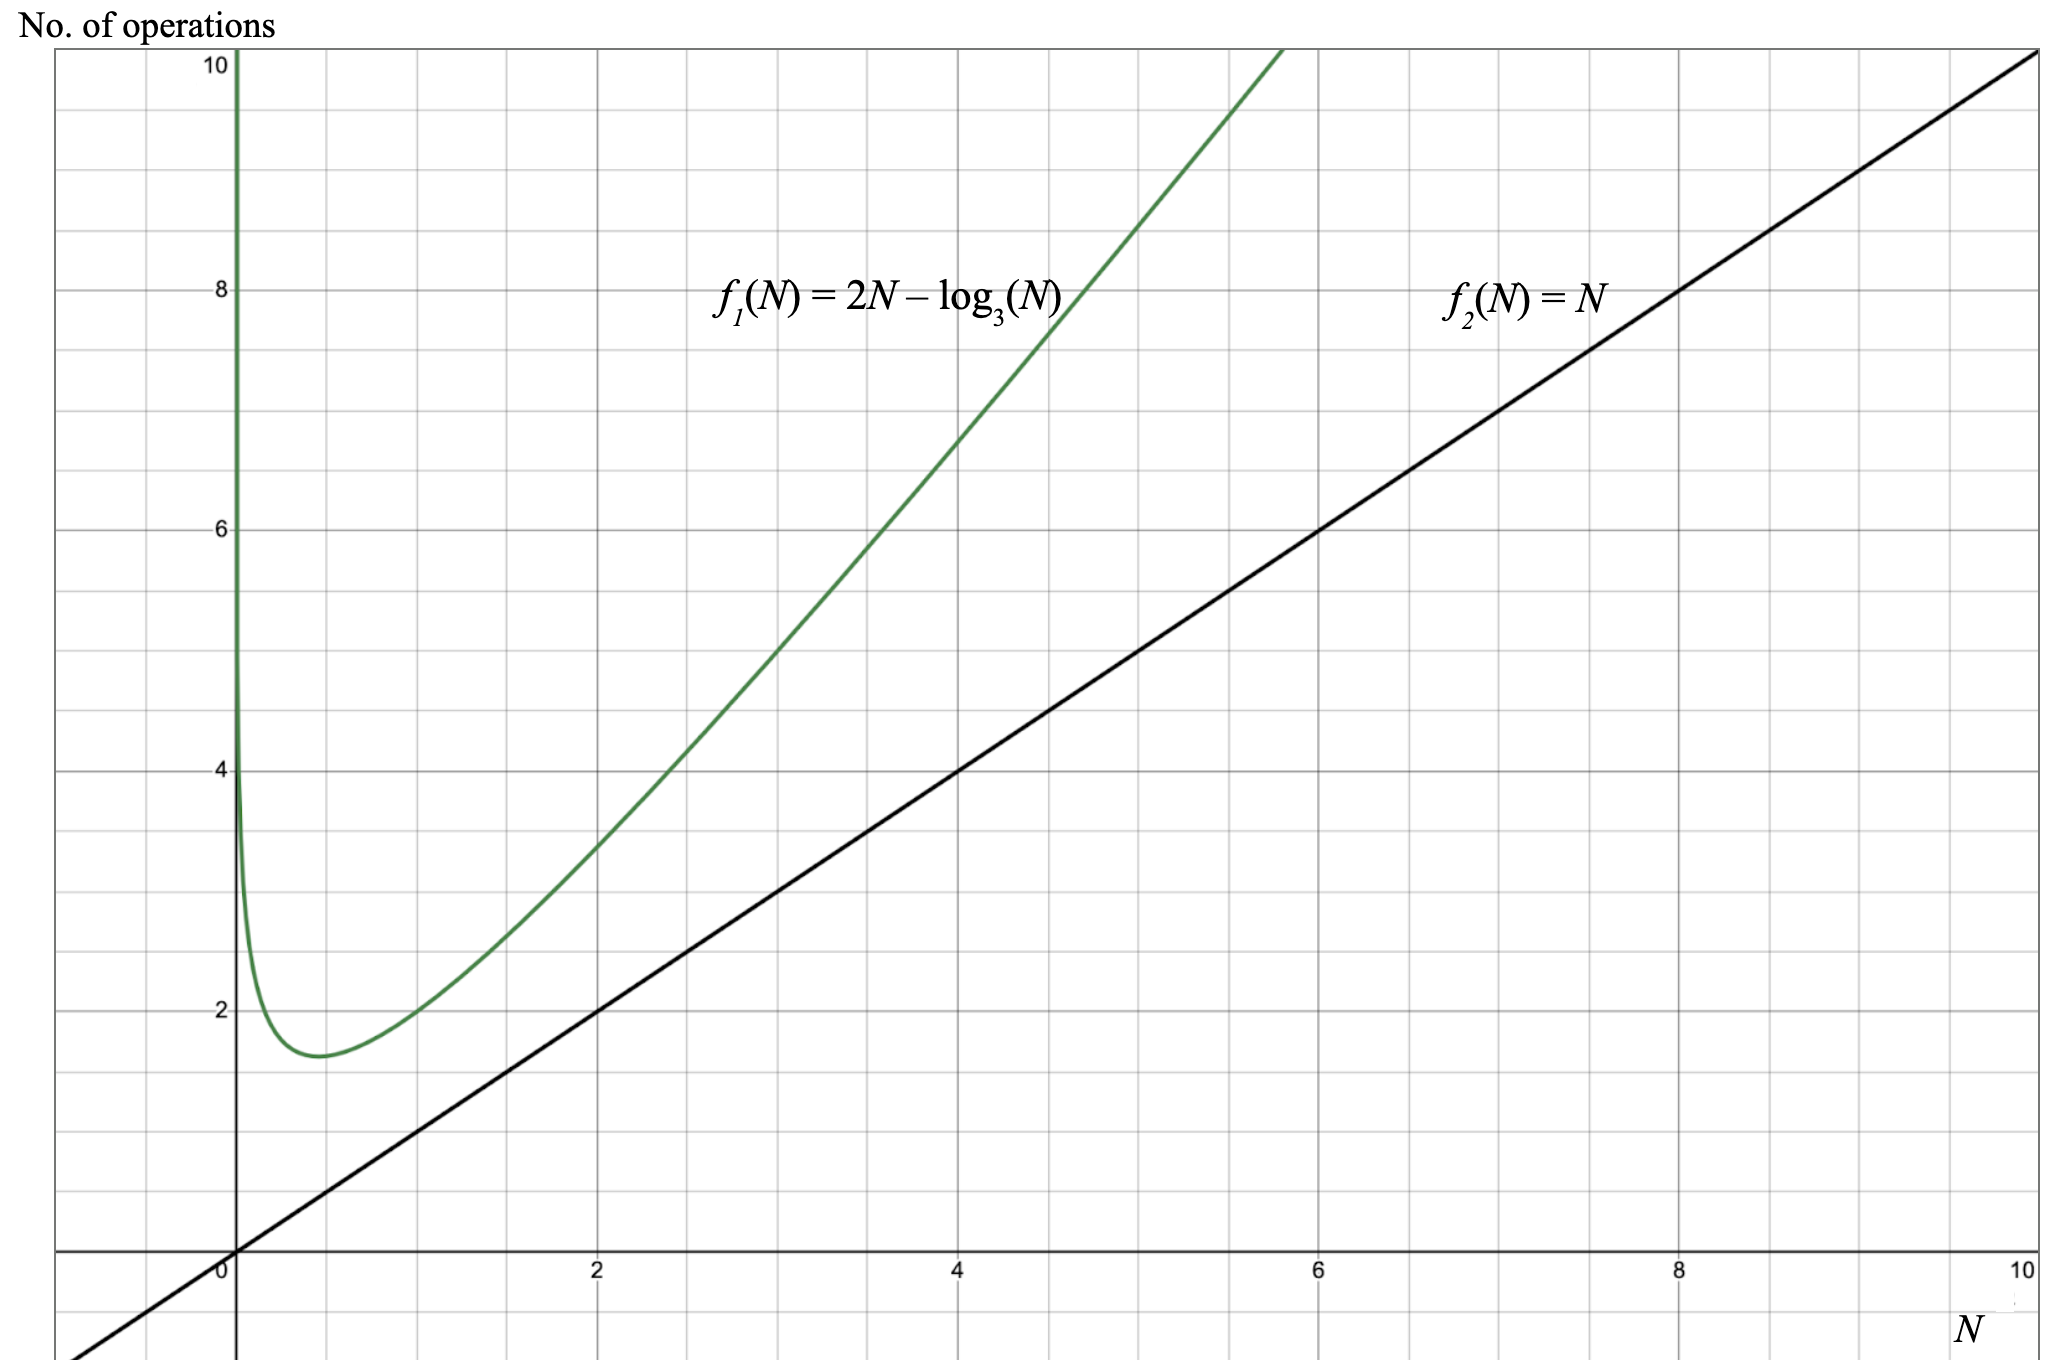
\includegraphics[width=0.9\linewidth]{Google Drawings/bigO-eg1-smalln-2.png}
    \label{fig:bigO-eg1-1}
\end{figure}

\vspace{-1em}
Shown in the figure above, $f_1(N)$ is clearly non-linear while $f_2(N)$ is, where:
\[D_f = \{N \in \mathbb{R}^+ \text{ } | \text{ } 0\leq N \leq 10 \}\]
The appearance of the functions seems to change for large values of $N$, where both visually appear linear, as demonstrated below.
\vspace{1em}

\begin{figure}[H]
    \centering
    \caption{Example functions for $t$ given large values of $N$}
    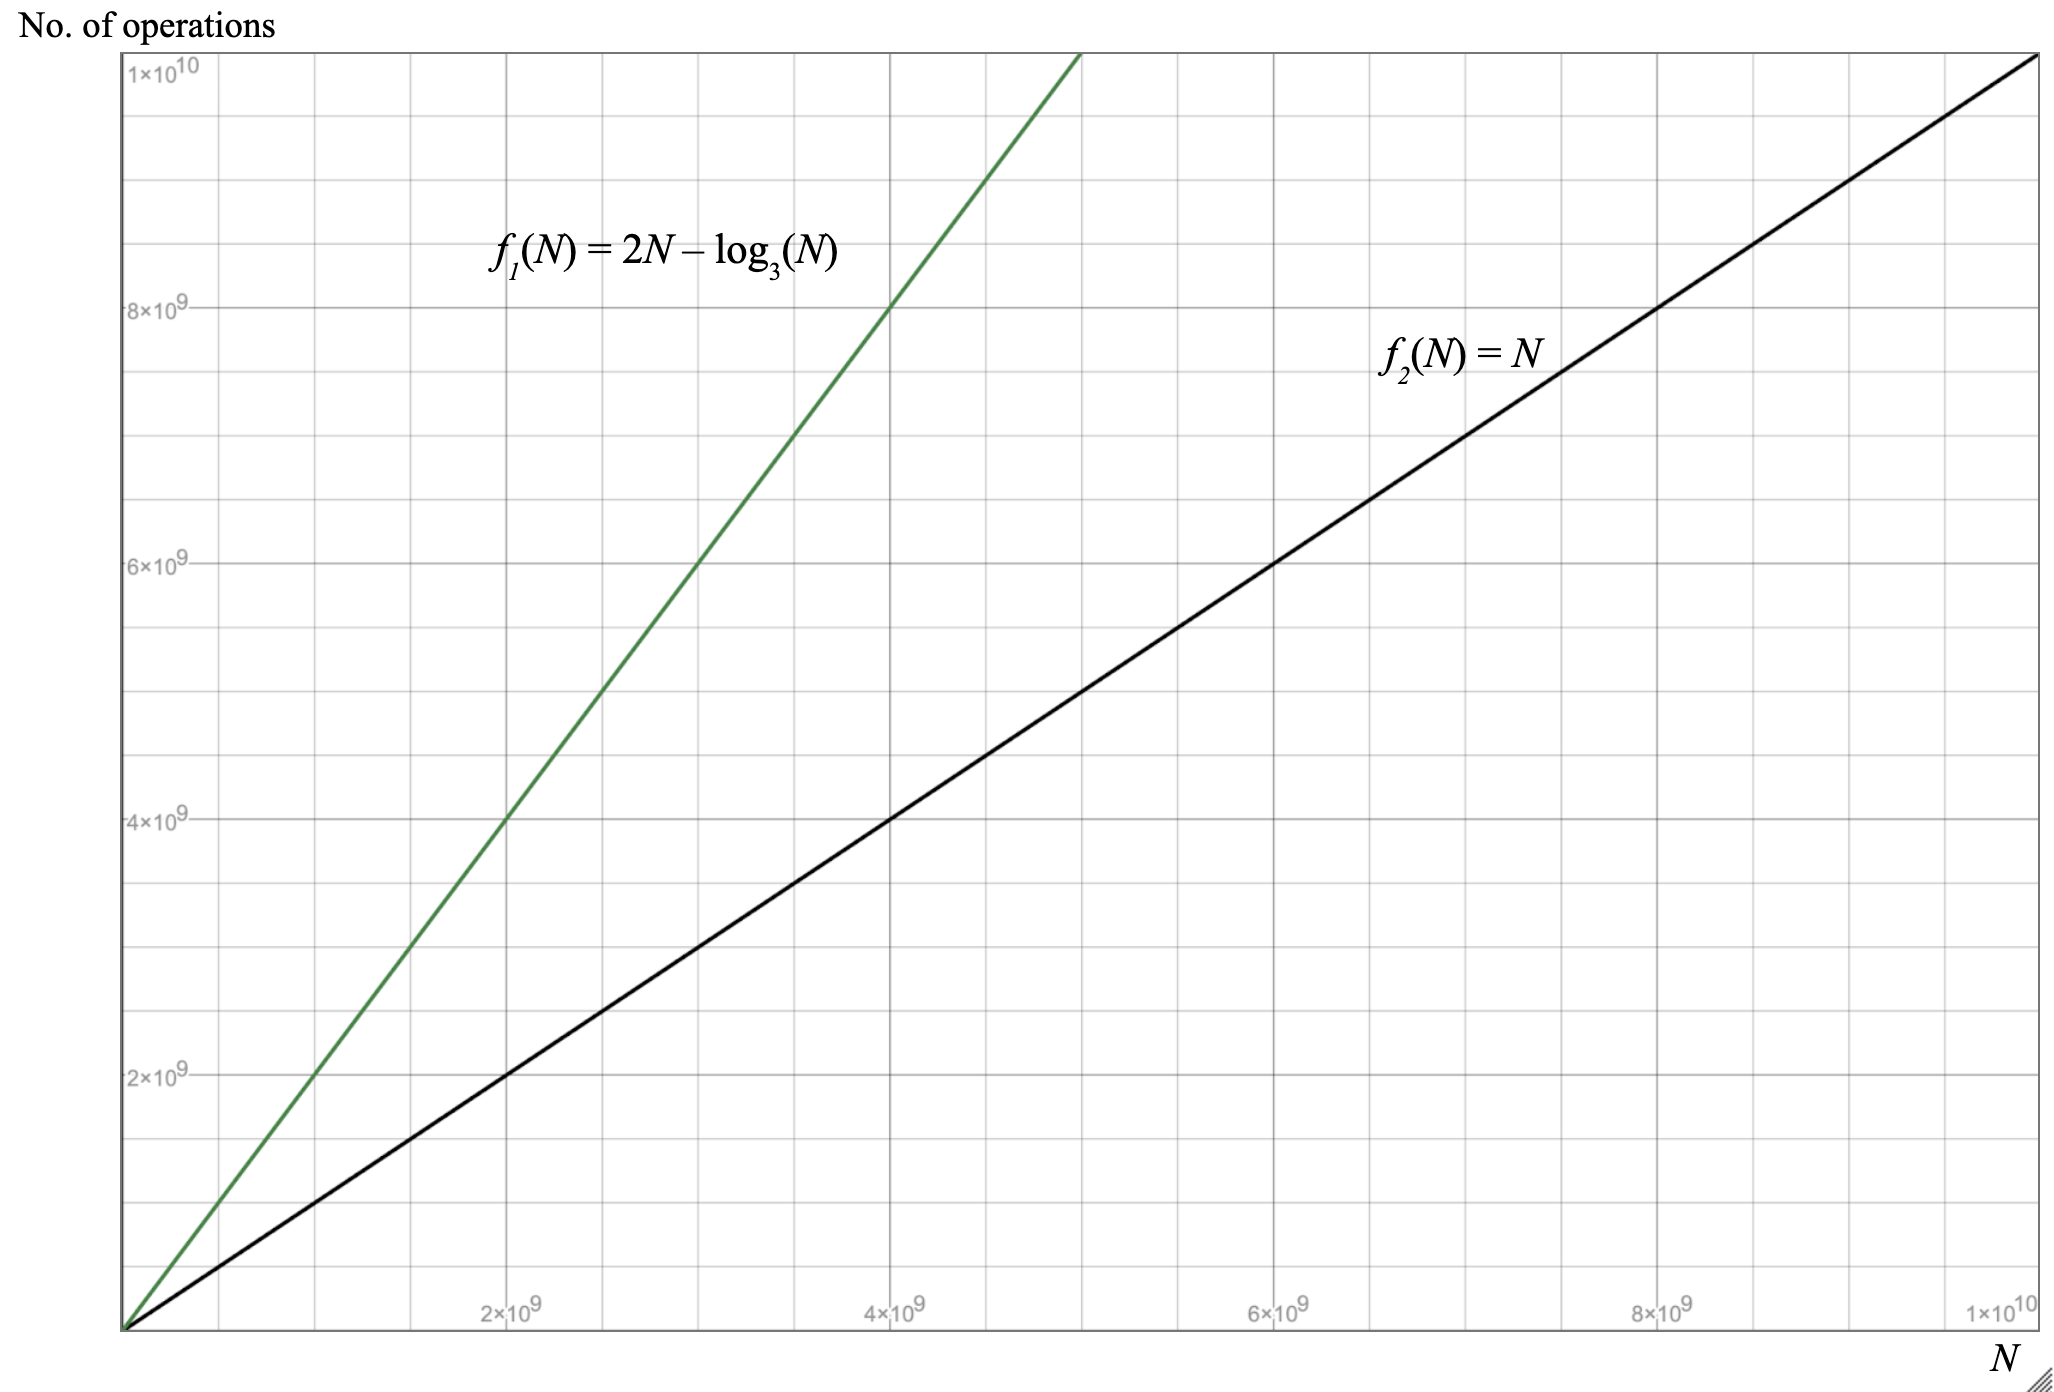
\includegraphics[width=0.9\linewidth]{Google Drawings/bigO-eg1-bign-2.png}
    \label{fig:bigO-eg1-2}
\end{figure}

In figure \ref{fig:bigO-eg1-2}, the functions $f_1(N)$ and $f_2(N)$ are drawn, where:
\[D_f = \{N \in \mathbb{R}^+ \text{ }|\text{ } 0\leq N \leq 10^{10}\}\]
which simulates large values of $N$, where both functions resemble a linear shape.\newline

Partially explained through the use of limits, when $N$ approaches infinity in $f_1(N)$, $2N\gg \log_3(N)$ and $\log_3(N)$ becomes insignificant when compared to $2N$, where $2N$ is the term with the highest OOG:\vspace{-1em}
\begin{align*}
    f_1(N)&=2N-\log_3(N)\\
    \lim_{N\to\text{ +}\infty} \frac{f_1(N)}{N}&=2
\end{align*}
According to the definition of the $O$-notation, since there does exist some constant $k$ where $kN \geq f_1(N)$, such as when $k=2$, for all large values of $N$, $f_1(N)$ has a linear OOG, which is $O(N)$. This also applies to $f_2(N)$, which has a linear OOG; the coefficient is a constant, $1$. Hence, the OOG of $f_1(N)$ is the same as the OOG of $f_2(N)$:

\vspace{-3em}
\begin{align*}
    f_1(N)&\in O(N)\\
    f_2(N)&\in O(N)
\end{align*}

Although $f_1(N)$ and $f_2(N)$ have different coefficients, they are said to have the same OOG because they have the same approximate \textbf{multiplicative change} as the input size $N$ changes. This property of the $O$-notation is examined below.

\subsubsection{Multiplicative change}
Consider the example in which $a(N) = 7N^2$ and $b(N) = 2N^2$, where both are OPS functions of separate algorithms. Although $a(N)$ and $b(N)$ have different coefficients of $N^2$, they are both elements of $O(N^2)$ as both algorithms have, approximately, the same multiplicative change when $N$ is large.\newline

In a scenario where $\beta=2N$ (input size $N$ is doubled), the multiplicative change between $a(N)$ and $a(\beta)$ would be such that $a(N) \times \text{multiplicative change} = a(\beta)$. Likewise, the same multiplicative change between $b(N)$ and $b(\beta)$ would be such that $b(N) \times \text{multiplicative change} = b(\beta)$ since $a(N)$ and $b(N)$ are both elements of $O(N^2)$.\newline

This specific scenario can be proven by first finding the multiplicative change, $\mu$, between $a(N)$ and $a(\beta)$:
\vspace{-2em}
\begingroup
\allowdisplaybreaks
\begin{align*}
    a(N) &= 7 N^2\\
    a(\beta) &= a(2N) = 7(2N)^2\\
    \vspace{0.5em}
    a(N) \times \mu &= a(\beta)\\
    (7 N^2) \times \mu &= 7(2N)^2\\
    7 \mu N^2 &= 28 N^2\\
    \mu &= \frac{28}{7}\\
    &= 4
\end{align*}
\endgroup
I get the same value of $\mu$ between $b(N)$ and $b(\beta)$:
\begingroup
\allowdisplaybreaks
\begin{align*}
    b(N) &= 2N^2\\
    b(\beta) &= b(2N) = 2(2N)^2\\
    \vspace{0.5em}
    b(N) \times \mu &= b(\beta)\\
    (2 N^2) \times \mu &= 2(2N)^2\\
    2 \mu N^2 &= 8 N^2\\
    \mu &= \frac{8}{2}\\
    &= 4
\end{align*}
\endgroup

In fact, it can be proven that any OPS function that is an element of $O(N^2)$ would have a multiplicative change of $4$ when the input of the function, $N$, is doubled. Let said function be expressed as:\newline

\begingroup
\onehalfspacing
\[\gamma(N) = kN^2 + \text{terms with an OOG lower than quadratic,}\]
\[\text{where $N$ is large and $k\in \mathbb{R}^+$}\]
\endgroup

And so,\vspace{-2em}

\begingroup
\allowdisplaybreaks
\onehalfspacing
\begin{align*}
    \gamma(N) \times \mu &\approx \gamma(2N)\\
    (kN)^2 \times \mu &= (k \times 2N)^2\\
    \mu k^2 N^2 &= 4 k^2 N^2\\
    \therefore \mu &= 4
\end{align*}
\endgroup

It is concluded that all elements of $O(N^2)$ would have approximately the same multiplicative change of $4$, where $N$ is already large, when its input size is doubled.\newline

Similar to how constant coefficients of $N$ do not affect functions' OOGs, in the context of the $O$-notation, the \textbf{base} of a logarithm also does not affect its OOG.

\subsubsection{The omission of the base of logarithms}
As you will see in figure \ref{fig:big-o-classification} within section \ref{use-of-O}, the bases of the logarithms in $O(\log (N))$ and $O(N \log (N))$ are omitted. While it implies the logarithm has a base of $2$ (due to the binary system in computer science), it can be shown that $\log_k(N) \in O(\log(N))$, where $k$ is a constant within the set of positive real numbers and $k \neq 1$.\newline

According to the \cite{ib}, $\log_a (x) = \frac{\log_b (x)}{\log_b (a)}$ where $a^x = b$ if and only if $x = \log_a (b)$, where $a > 0$ and $b > 0$ and $a \neq 1$. Hence:
\begingroup
\onehalfspacing
\begin{align*}
    \log_k(N) &= \frac{\log(N)}{\log(k)}\\
    &= \frac{1}{\log(k)} \times \log(N)\\
    &\in O(\log(N))\quad \because \text{ $\frac{1}{\log(k)}$ is a constant}
\end{align*}
\endgroup
Because $\log_k(N)$ is $\log (N)$ multiplied by a constant, the constant base of a logarithm in the context of the OOG is irrelevant.\newline

Note that this holds true for elements of $O(N\log(N))$, where:
\[N\log_k (N) = \frac{1}{\log(k)} N\log(N) \in O(N\log (N))\]

\subsection{Use of $O$-notation in this essay}\label{use-of-O}
A computer algorithm would be considered as faster if its OPS function, given large inputs, had a smaller OOG, illustrated in the diagram below \parencite{huang_2020_big_O}.

\begin{figure}[H]
    \centering
    \caption{Classifications of different orders of growth}
    \hspace{-2em}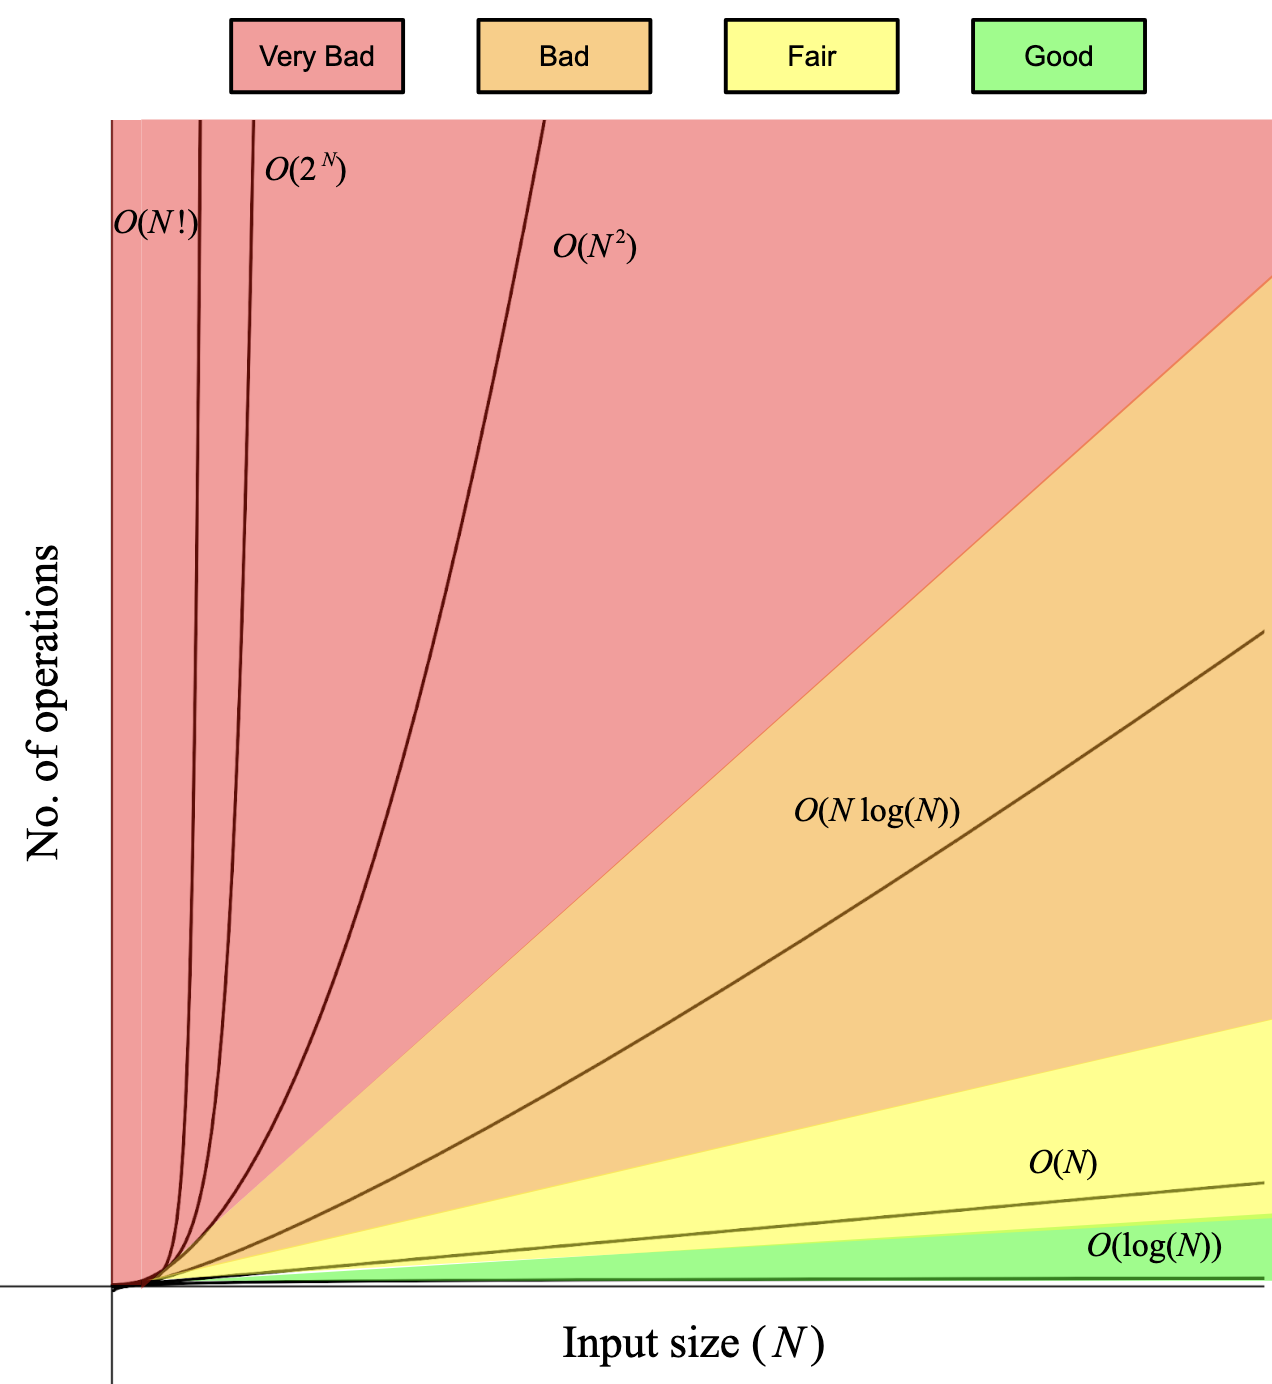
\includegraphics[width=0.75\linewidth]{Google Drawings/graph-bigo-2.png}
    \label{fig:big-o-classification}
\end{figure}
\vspace{-27pt}
\bgroup
\scriptsize
\begin{center}
    Interpreted from: https://www.freecodecamp.org/news/big-o-notation-why-it-matters-and-why-it-doesnt-1674cfa8a23c/
\end{center}
\egroup

The different OOGs will be used to describe and compare the speeds of algorithms, such as algorithms that create binary heap, as seen in but not limited to sections \ref{williams_OOG}, \ref{floyds_OOG} and \ref{conclusion}.\newline
%The number of operations an algorithm takes for different input sizes is critical as it largely determines the time taken for a procedure to be completed since computers take a rather constant amount of time to process each operation \parencite{pc_takes_time}. Therefore, the terms ``number of operations" and ``amount of time" will be used interchangeably throughout this essay.\newline

Next, the role of binary heaps in relation to priority queues is discussed.

\section{The priority queue}\label{priority_queue}
Priority queues are made up of elements such as numbers or characters that have differing levels of priority, usually represented numerically \parencite{cornell_fall_2020}. Priority queues can exist as a sorted or unsorted sequence of elements \parencite{cornell_fall_2020}. The diagram below illustrates an example of a priority queue, used to triage patients, where the value of an element is the patient’s name and their urgency for medical attention is a range of integers, sorted in descending order.\newline

\begin{figure}[H]
    \centering
    \caption{Priority queue (sorted) of an example triage system}
    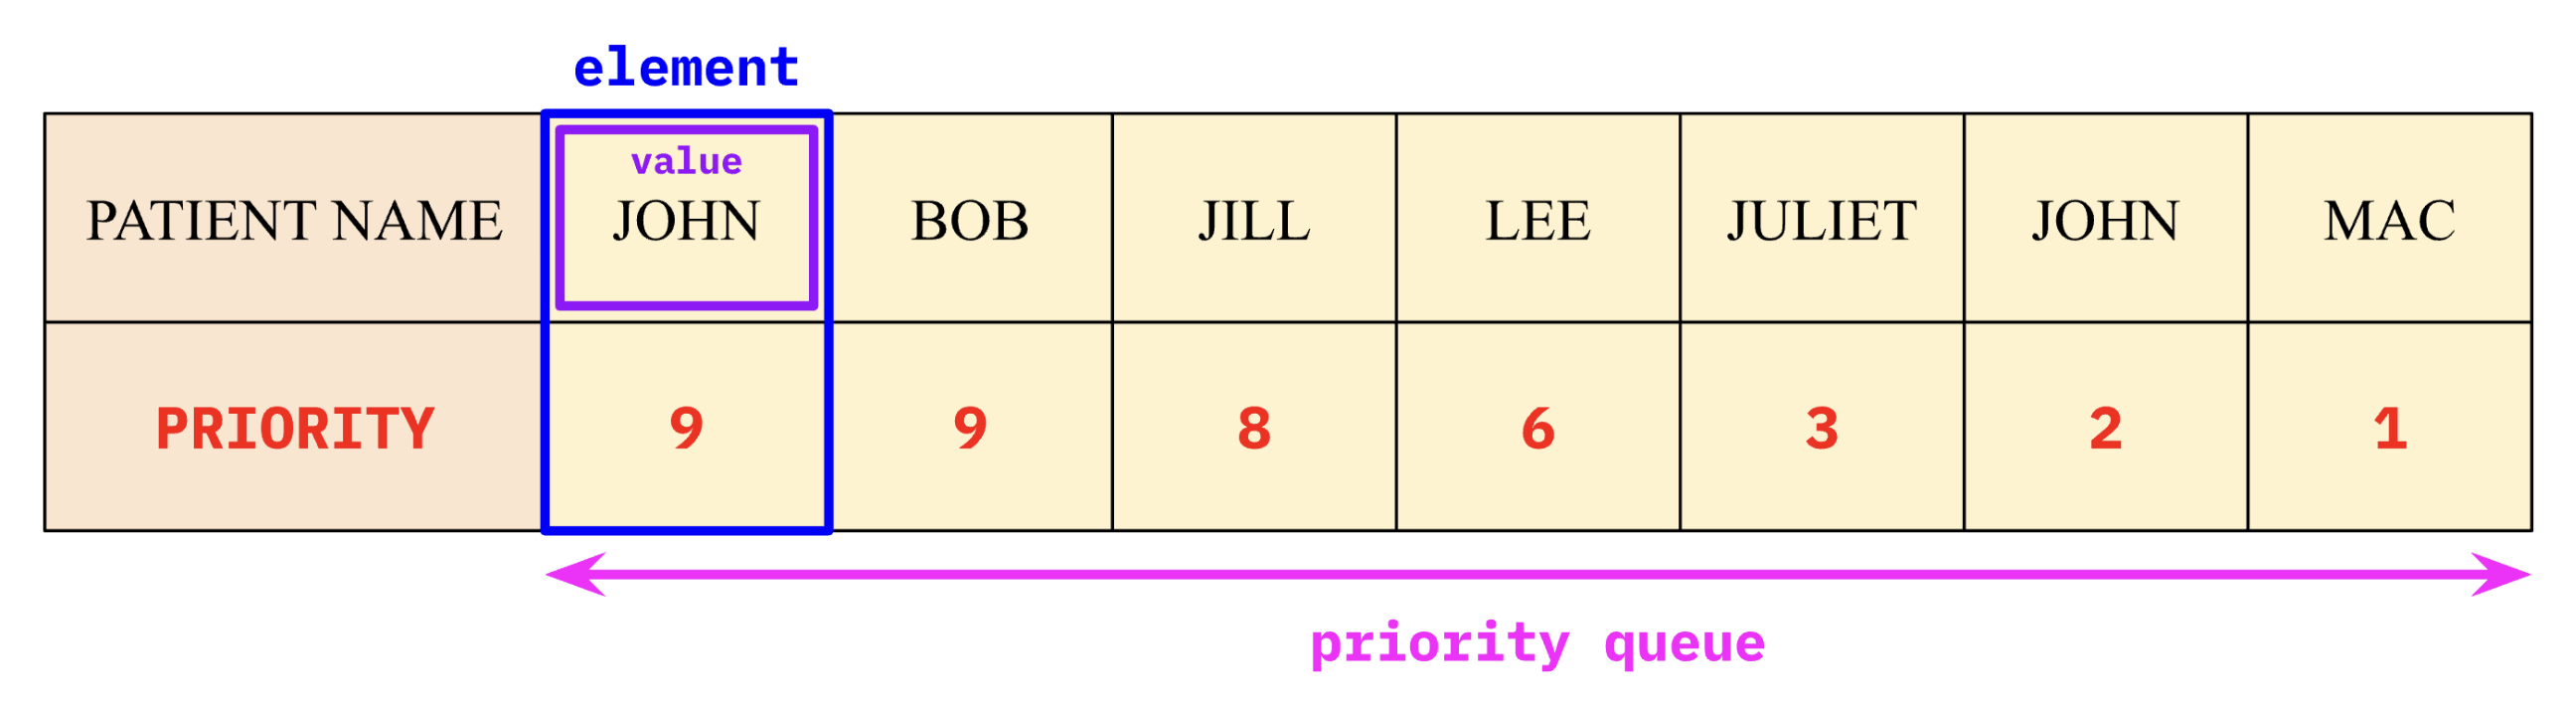
\includegraphics[width=0.75\linewidth]{Google Drawings/triage-queue.png}
    \label{fig:triage-queue}
\end{figure}

The value the elements contain do not affect the order of the priority queue; it is only ordered by the element’s priority. It will therefore be omitted from future illustrations.\newline

In a priority queue that is implemented through a sequence of sorted elements, the computer procedure of retrieving the highest and lowest priority elements is the fastest as they are located on each end of the queue while the process of inserting new elements into the queue may require the queue to be rearranged to remain sorted.\newline

In figure \ref{fig:pq-rearrange-example}, an element of priority $10$ was added to the back of the priority queue, which was made up of a sorted sequence of elements, in descending order.\vspace{1em}

\begin{figure}[H]
    \centering
    \caption{Example of a priority queue of sorted elements that needs to be rearranged}
    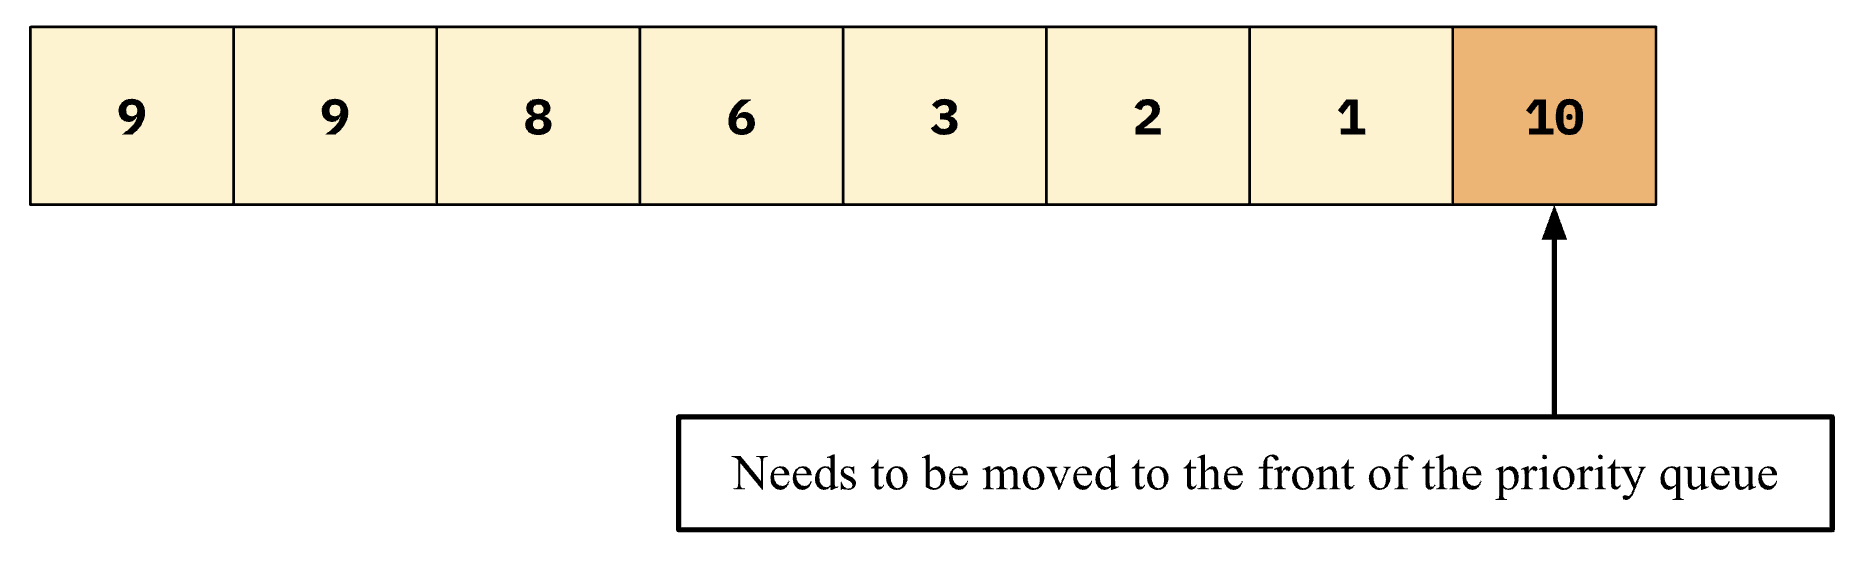
\includegraphics[width=0.75\linewidth]{Google Drawings/sorted-queue-move.png}
    \label{fig:pq-rearrange-example}
\end{figure}

Since the element which was just added had a higher priority than all other elements that were in the queue, it has to be shifted to the front of the priority queue, affecting the position of all elements in the queue. Because of this, adding an element would be slower than the retrieval of the highest and lowest priority elements.\newline

Priority queues can also be implemented using a sequence of unsorted elements \parencite{cornell_fall_2020}. In a sequence of unsorted elements, it is faster to add new elements to the existing priority queue as the elements’ order does not matter while it is slower to retrieve the element with the highest priority as a search for the element is required since it may not be found at either end of the queue.\newline

While a priority queue can be represented by a sequence of elements as seen in figure \ref{fig:triage-queue}, it can also be expressed in the form of a tree called a binary heap.

\subsection{Binary heap representation of priority queues}\label{pq_as_bin}
In a binary heap, elements are represented as nodes. Figure \ref{fig:pq-heap-first} illustrates a max binary heap, where the top most node holds the highest priority \parencite{mit_pq_info}. On the other hand, a min heap would have the top most node holding the lowest priority \parencite{nus}.

\begin{figure}[H]
    \centering
    \caption{Binary heap implementation of a priority queue}
    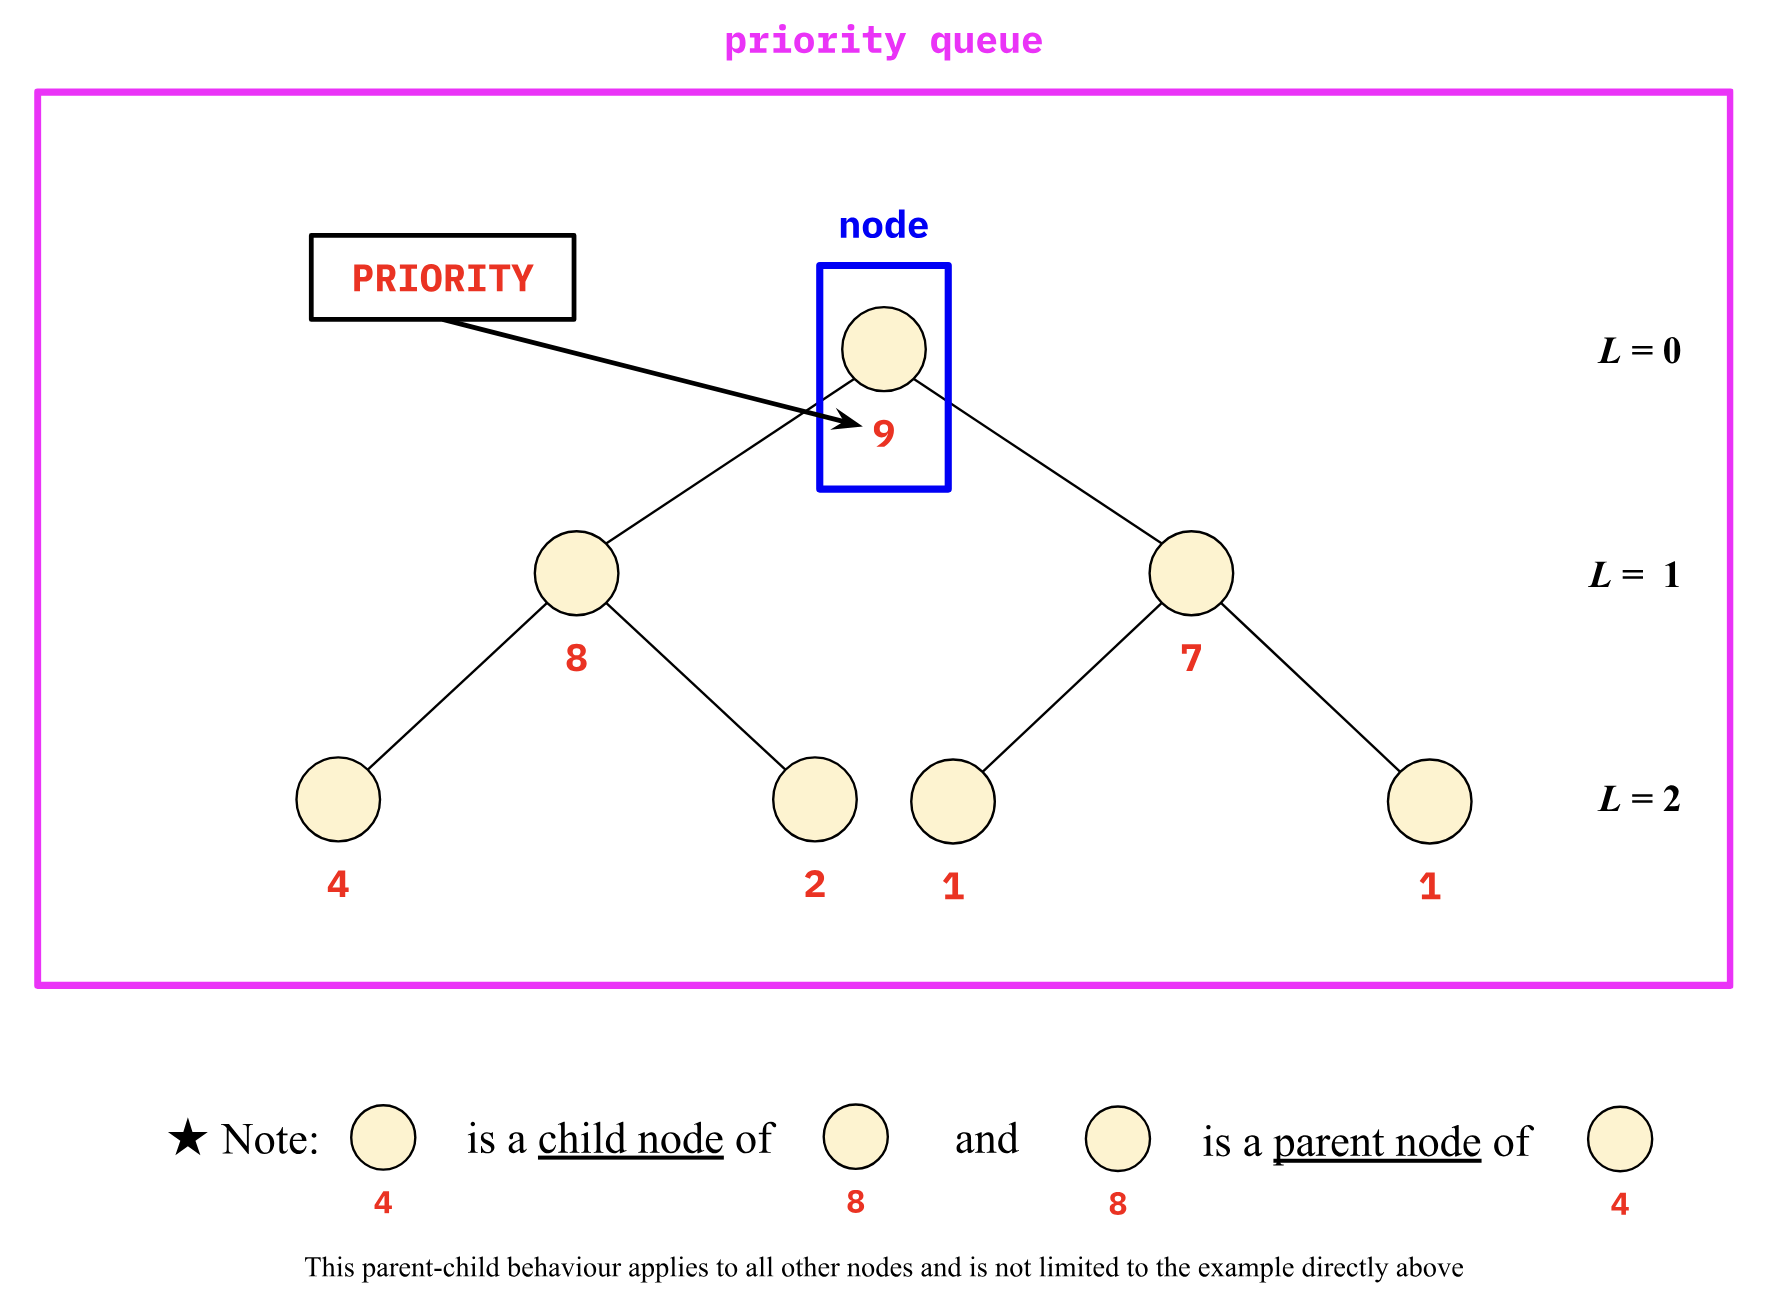
\includegraphics[width=0.75\linewidth]{Google Drawings/pq-heap-intro-v2.png}
    \label{fig:pq-heap-first}
\end{figure}

In figure \ref{fig:pq-heap-first}, the nodes are split into different levels, starting from $0$. All binary heaps would have $2^L$ nodes at level $L$, for every level, except its lowest level which would have between $1$ to $2^L$ nodes, inclusive \parencite{cornell_fall_2020}. For ease of explanations, only max binary heaps that have $2^L$ nodes in their lowest level will be used throughout this investigation. Nodes connected to another node with a higher priority are called \textbf{child nodes}, with the higher priority nodes being called \textbf{parent nodes} \parencite{cornell_fall_2020}. The node at the top of the binary heap is called the \textbf{root node} \parencite{cornell_fall_2020}. In order for a binary heap to be valid, all parent nodes in a max heap must not have a lower priority than both its child nodes \parencite{cornell_fall_2020}.\newline

The maximum level a heap has is referred to as its height, $H$. The relationship between the total number of nodes, $N$, and $H$ is shown in the table below so that it can be utilised in later calculations.\vspace{0.5em}

\begin{table}[H]
    \centering
    \caption{Relationship of $N$ and $H$}
    \bgroup
    \setlength{\tabcolsep}{15pt}
    \renewcommand{\arraystretch}{1.1}
    \begin{tabular}{|c|c|c|c|c|c|c|c|}
        \hline
        $H$ & $0$ & $1$ & $2$ & $3$ & $4$ & \dots & $h$\\
        \hline
        $N$ & $1$ & $3$ & $7$ & $15$ & $31$ & \dots & $N_h$\\
        \hline
    \end{tabular}
    \egroup
    \label{tab:Rel-N&H}
\end{table}

Though table \ref{tab:Rel-N&H} does not provide a sequence of numbers that is arithmetic or geometric, I realised that $N$ had values that were close to the powers of $2$. By adding $1$ to all values of $N$, we can now view table \ref{tab:Rel-N+1&H} as a geometric sequence with a common ratio of $2$.

\begin{table}[H]
    \centering
    \caption{Relationship of $N+1$ and $H$}
    \bgroup
    \setlength{\tabcolsep}{15pt}
    \renewcommand{\arraystretch}{1.1}
    \begin{tabular}{|c|c|c|c|c|c|c|c|}
        \hline
        $H$ & $0$ & $1$ & $2$ & $3$ & $4$ & \dots & $h$\\
        \hline
        $N+1$ & $2$ & $4$ & $8$ & $16$ & $32$ & \dots & $N_h+1$\\
        \hline
    \end{tabular}
    \egroup
    \label{tab:Rel-N+1&H}
\end{table}

With the use of $u_n=u_1r^{n-1}$, which is the formula to find the $n$th term of a geometric sequence where $u_1$ is the first term of the sequence and $r$ is the common ratio, I can now express $H$ in terms of $N$ as shown in \eqref{eqn:H_ito_N} and vice versa in equation \ref{eqn:N_ito_H} \parencite{ib}.
\vspace{-2em}

\bgroup
\allowdisplaybreaks
\onehalfspacing
\begin{align}
    u_n&=u_1r^{n-1} \nonumber\\
    N+1&=2\times2^H \nonumber\\
    N+1&=2^{H+1} \nonumber \\
    N&=2^{H+1}-1 \label{eqn:N_ito_H}\\
    H+1&=\log_2(N+1) \nonumber \\
    H&=\log_2(N+1)-1 \label{eqn:H_ito_N}
\end{align}
\egroup

Equations \ref{eqn:N_ito_H} and \ref{eqn:H_ito_N} will be used in future calculations, such as to find the OPS functions of Williams's method and Floyd's method.\newline

This essay focuses on priority queues as binary heaps instead of priority queues as sequences of numbers as it generally takes a smaller number of operations to complete for a combination of operations, discussed in the next section.

\subsection{Advantage of binary heaps}\label{advantage_of_binary_heaps}
Table \ref{tab:BH-vs-Array} contains the OOG of the OPS functions for the insertion or removal of the element with the highest priority from a priority queue of $N$ elements that has been implemented through a binary heap, a sorted sequence of elements and a completely unsorted sequence of elements.\vspace{1em}

\begin{table}[H]
    \centering
    \caption{OOGs of OPS functions for insertion and removal operations}
    \vspace{-1em}
    \bgroup
    \singlespacing
    \small
    \renewcommand\tabularxcolumn[1]{m{#1}} % v-center
    \renewcommand{\arraystretch}{1.1}
    \begin{tabularx}{\textwidth}{|X|X|X|X|}
        \hline
        $ $ & \Centering{Binary heap} & \Centering{Sorted sequence of elements} & \Centering{Unsorted sequence of elements}\\
        \hline
        \RaggedRight{OOG of the OPS function to insert a new element} & \Centering{$O(\log(N))$} & \Centering{$O(N)$} & \Centering{$O(1)$}\\
        \hline
        \RaggedRight{OOG of the OPS function to remove the highest priority element} & \Centering{$O(\log(N))$} & \Centering{$O(1)$} & \Centering{$O(N)$}\\
        \hline
    \end{tabularx}
    \egroup
    \label{tab:BH-vs-Array}
\end{table}
\vspace{-26.5pt}
\bgroup
\scriptsize
\begin{center}
    Values in the "Binary heap" column are according to \cite{mit_pq_info} and the \cite{nus}
\end{center}
\egroup

Recalling the explanations of a sorted sequence of elements and an unsorted sequence of elements from section \ref{priority_queue} and with reference to table \ref{tab:BH-vs-Array}, an OOG of $O(N)$ indicates that a search involving multiple operations is required while an OOG of $O(1)$, indicates a constant number of operations is required.\newline

The nature of the different values within table \ref{tab:BH-vs-Array} is examined with figures \ref{fig:arr-swaps} and \ref{fig:bh-swaps}, where an element with priority $9$ is added to a sorted sequence of elements and a binary heap, both with $7$ existing elements in it. \newline

\begin{figure}[H]
    \centering
    \caption{Illustration of insertion procedure in a sorted sequence of elements}
    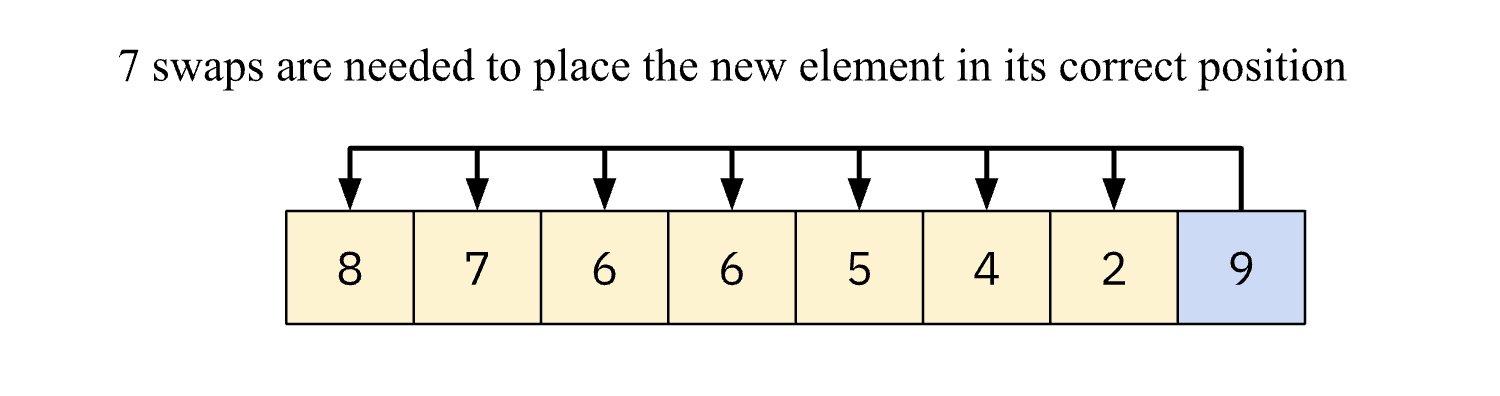
\includegraphics[width=0.75\linewidth]{Google Drawings/arr-swaps.png}
    \label{fig:arr-swaps}
\end{figure}

\begin{figure}[H]
    \centering
    \caption{Illustration of insertion procedure in a binary heap}
    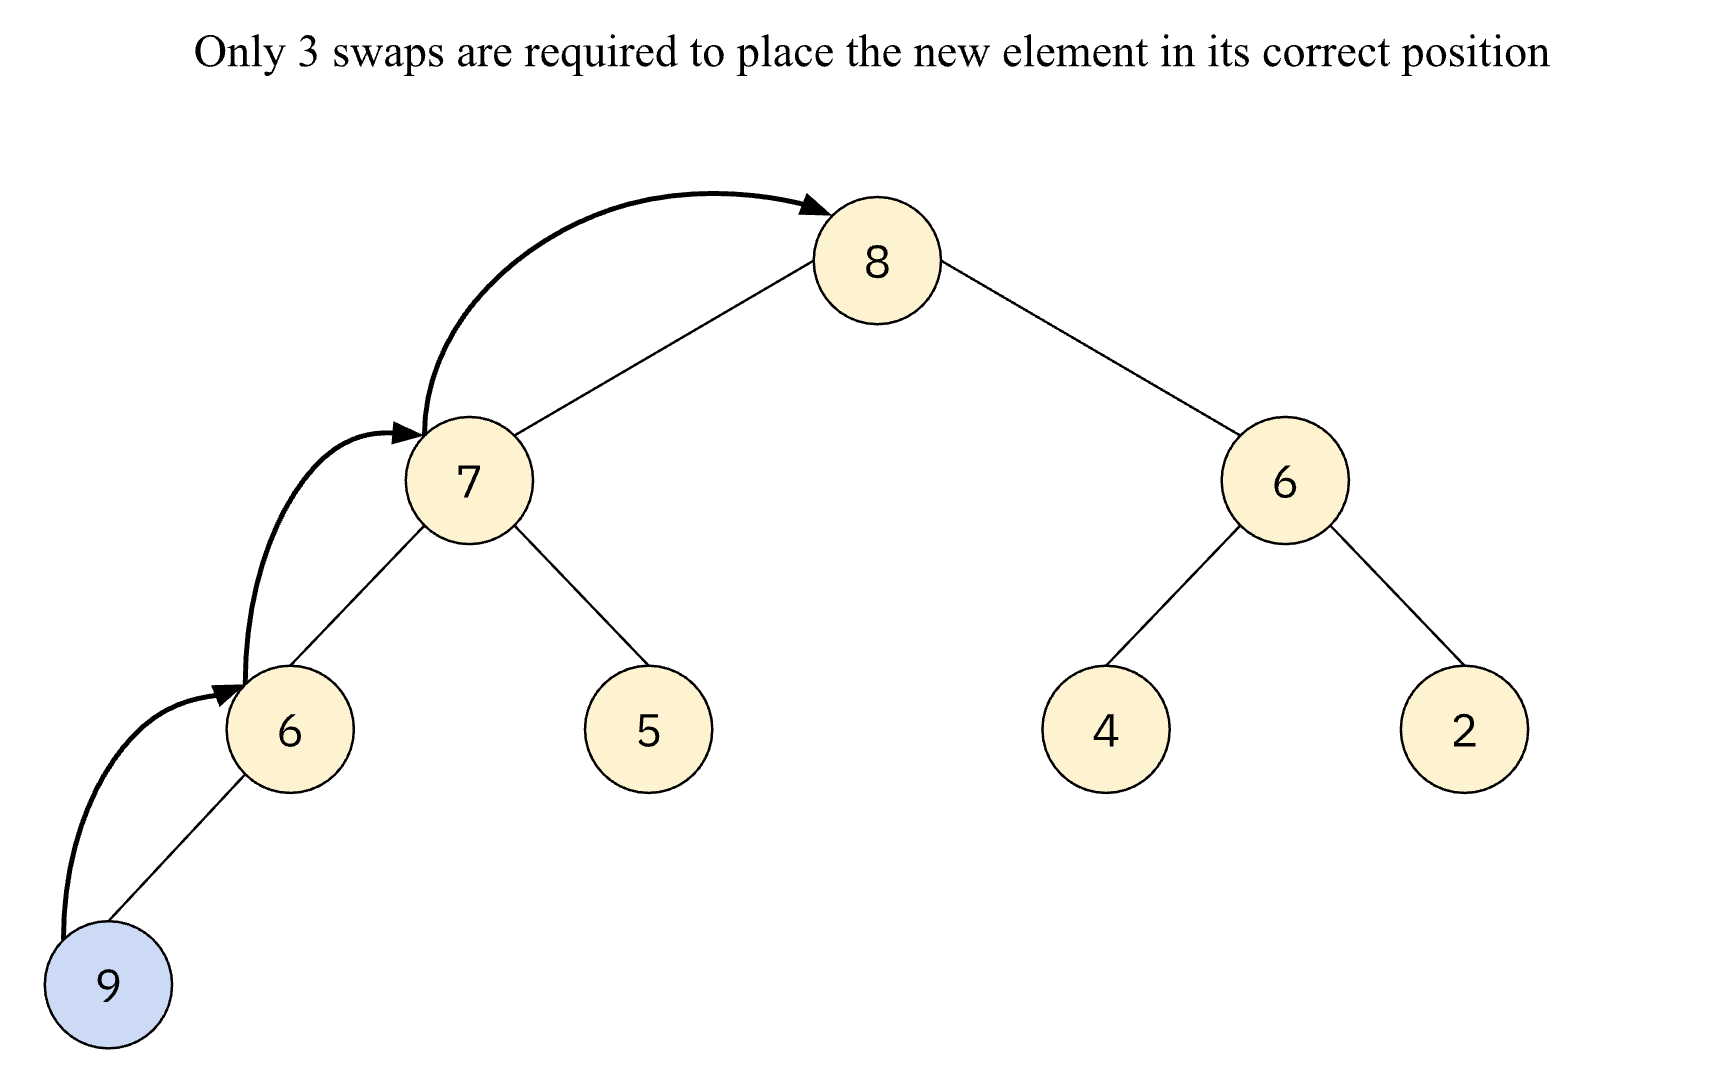
\includegraphics[width=0.75\linewidth]{Google Drawings/bh-swaps.png}
    \label{fig:bh-swaps}
\end{figure}

In figure \ref{fig:arr-swaps}, it took $7$ swaps to place the newly-added $8$th element in its correct position while the binary heap in figure \ref{fig:bh-swaps} only took $3$ swaps. With each swap considered as an operation, the binary heap required less operations for insertion when compared to a sorted sequence of elements.\newline

Combining the values of the insertion and removal procedures from table \ref{tab:BH-vs-Array},

\begingroup
\onehalfspacing
\allowdisplaybreaks
\begin{center}
    OOG of combined procedures in binary heaps\vspace{0.5em}
\end{center}
\vspace{-2em}
\begin{align*}
    &\equiv O(\log N) + O(\log N)\\
    &\equiv 2\times O(\log N)\\
    &\equiv O(\log N)
\end{align*}
\begin{center}
    OOG of combined procedures in sequence of numbers\vspace{0.5em}
\end{center}
\vspace{-2em}
\begin{align*}
    &\equiv O(1) + O(N)\\
    &\equiv k + O(N), \quad k\in \mathbb{R^+}\\
    &\equiv O(N)
\end{align*}
\endgroup
\vspace{-1.5em}

For the same mix of operations and input size, the OOG of the combined procedures in binary heaps is generally less than the OOG of the combined procedures in a sequence of numbers, whether unsorted or sorted. This difference grows as $N$ increases, shown in the figure below.\vspace{0.5em}

\begin{figure}[H]
    \centering
    \caption{Growth in difference between $O(N)$ and $O(\log N)$}
    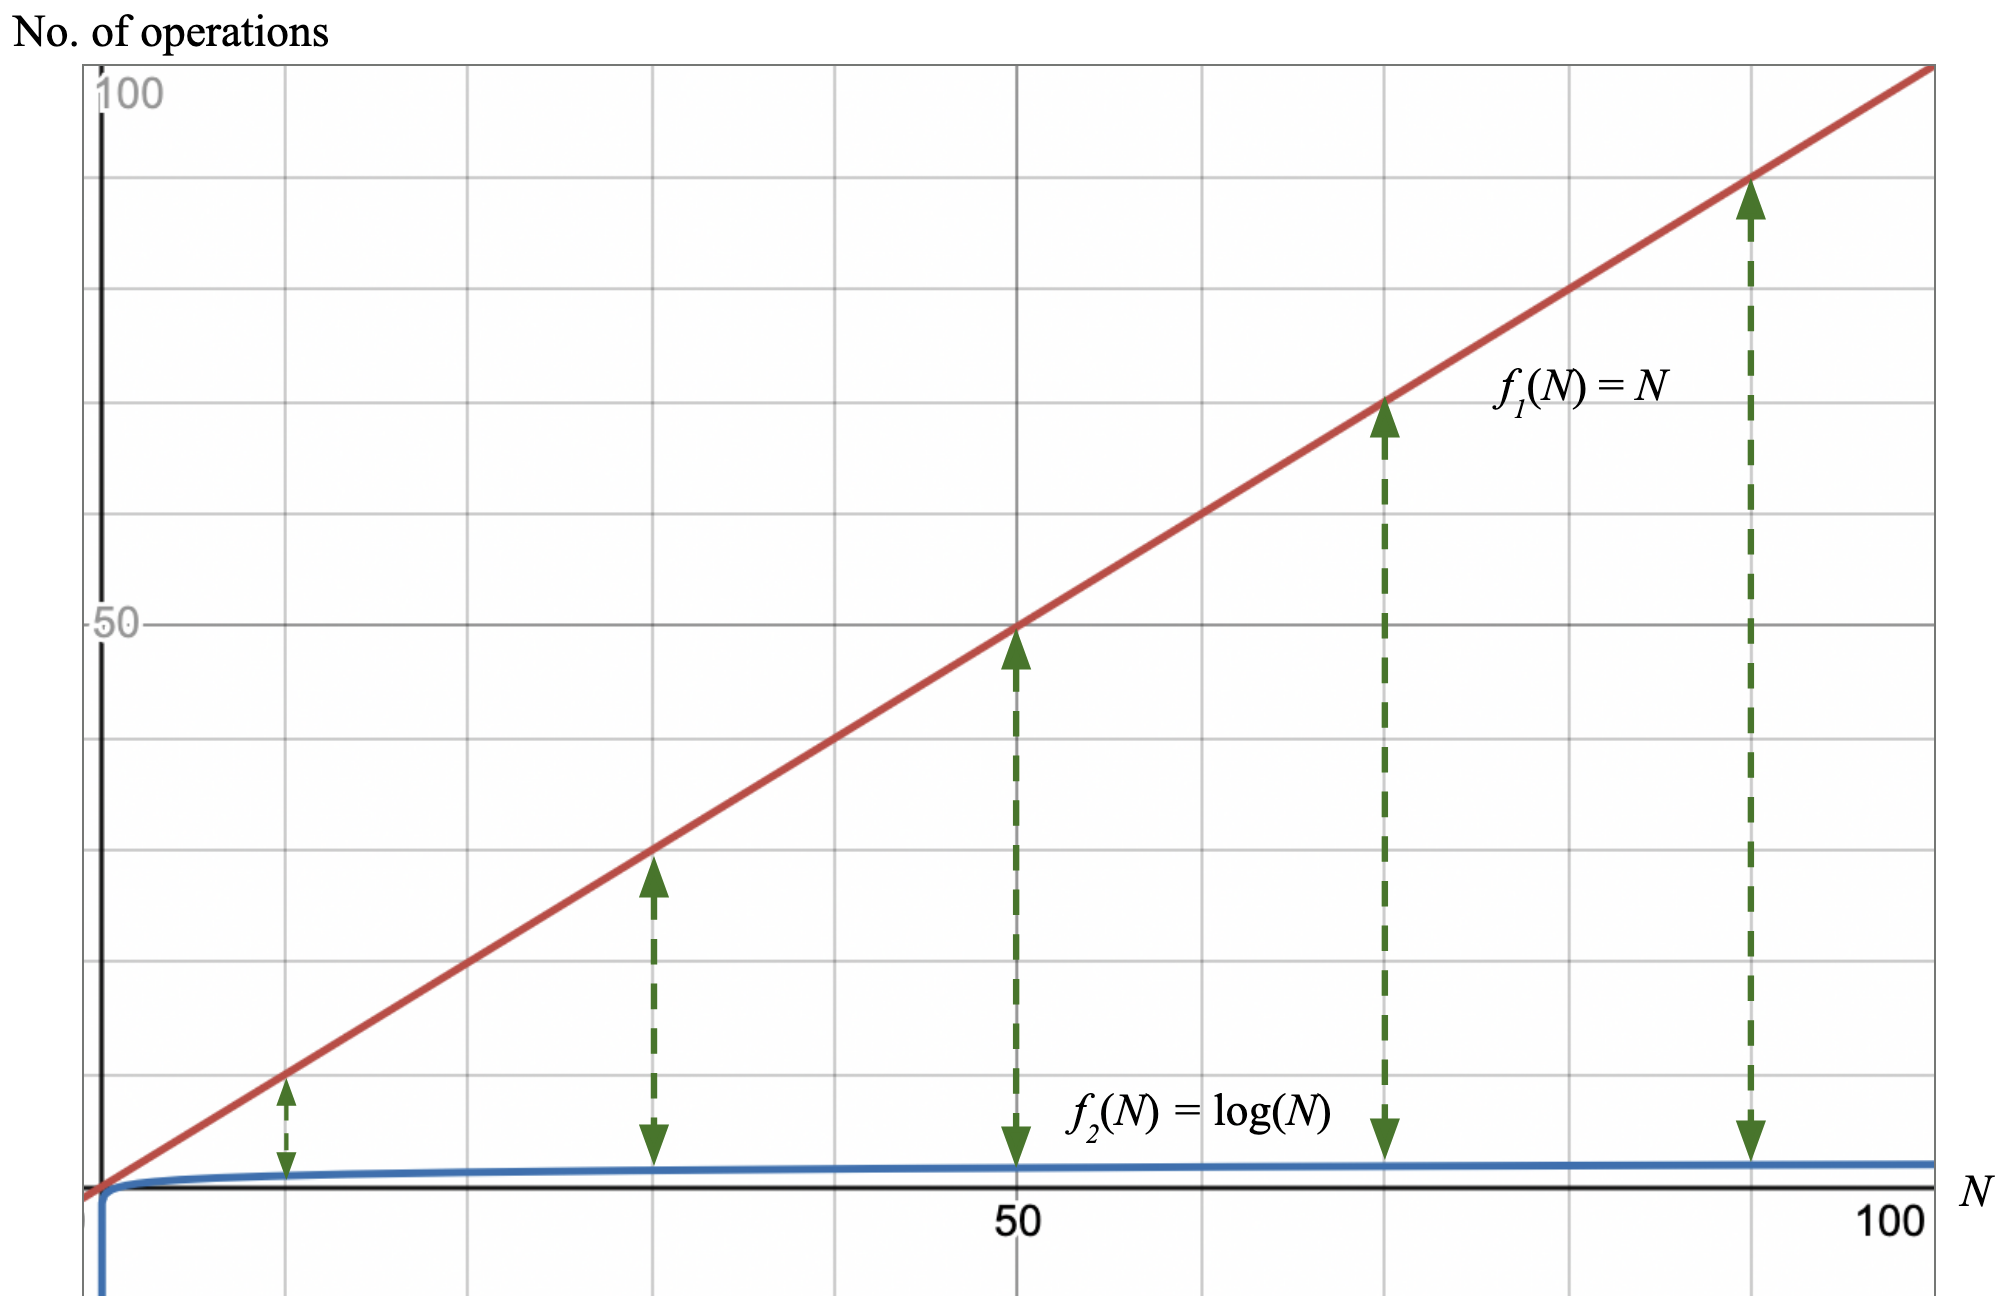
\includegraphics[width=0.9\linewidth]{Google Drawings/linear-grows-more-than-log.png}
    \label{fig:linear-vs-log-growth}
\end{figure}

Note that, in figure \ref{fig:linear-vs-log-growth}, $f_1(N) \in O(N)$ and $f_2(N) \in O(\log N)$, with the green dotted lines representing the rough difference between the output of $f_1(N)$ and $f_2(N)$ for different values of $N$.\newline

While binary heaps are shown to provide faster procedures in a priority queue, the procedures of creating a binary heap were also improved \parencite[58]{JCC}.

\section{Williams's binary heap creation method}
Initially, binary heaps were created through the use of J.W.J. Williams’s method by inserting each element one after the other \parencites[4]{nus}[58]{JCC}. Binary heaps are always filled from left to right, only creating a new level when the lowest level is full; the number of nodes at the lowest level is exactly $2^L$, for the purpose of this essay \parencite{cornell_fall_2020}.\newline

An example of how a binary heap is created through the use of Williams's method is demonstrated in figure \ref{fig:williams-creation}. Numbers that have not been added to the binary heap are marked with a yellow background while numbers that have already been added to the binary heap are marked with a green background.

\clearpage
\begin{figure}[H]
    \centering
    \caption{Creation of a binary heap through Williams’s method}
    \label{fig:williams-creation}
    \begin{subfigure}{\textwidth}
        \centering
        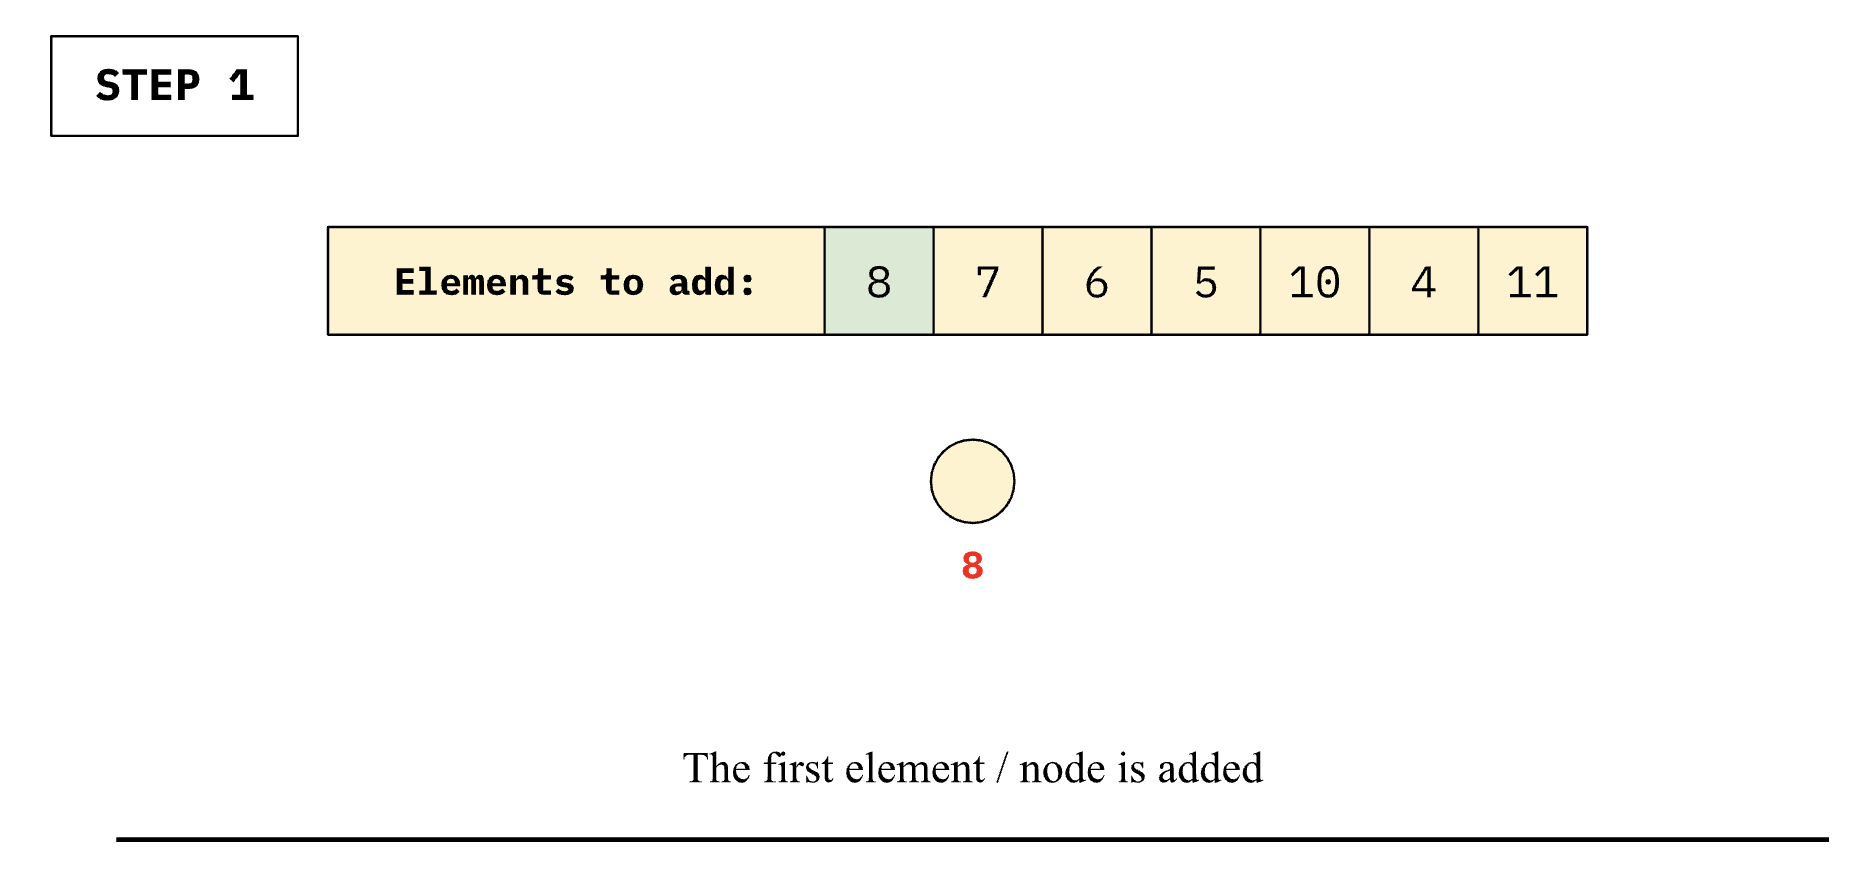
\includegraphics[width=0.8\linewidth]{Google Drawings/williams-1.png}
    \end{subfigure}
    \begin{subfigure}{\textwidth}
        \centering
        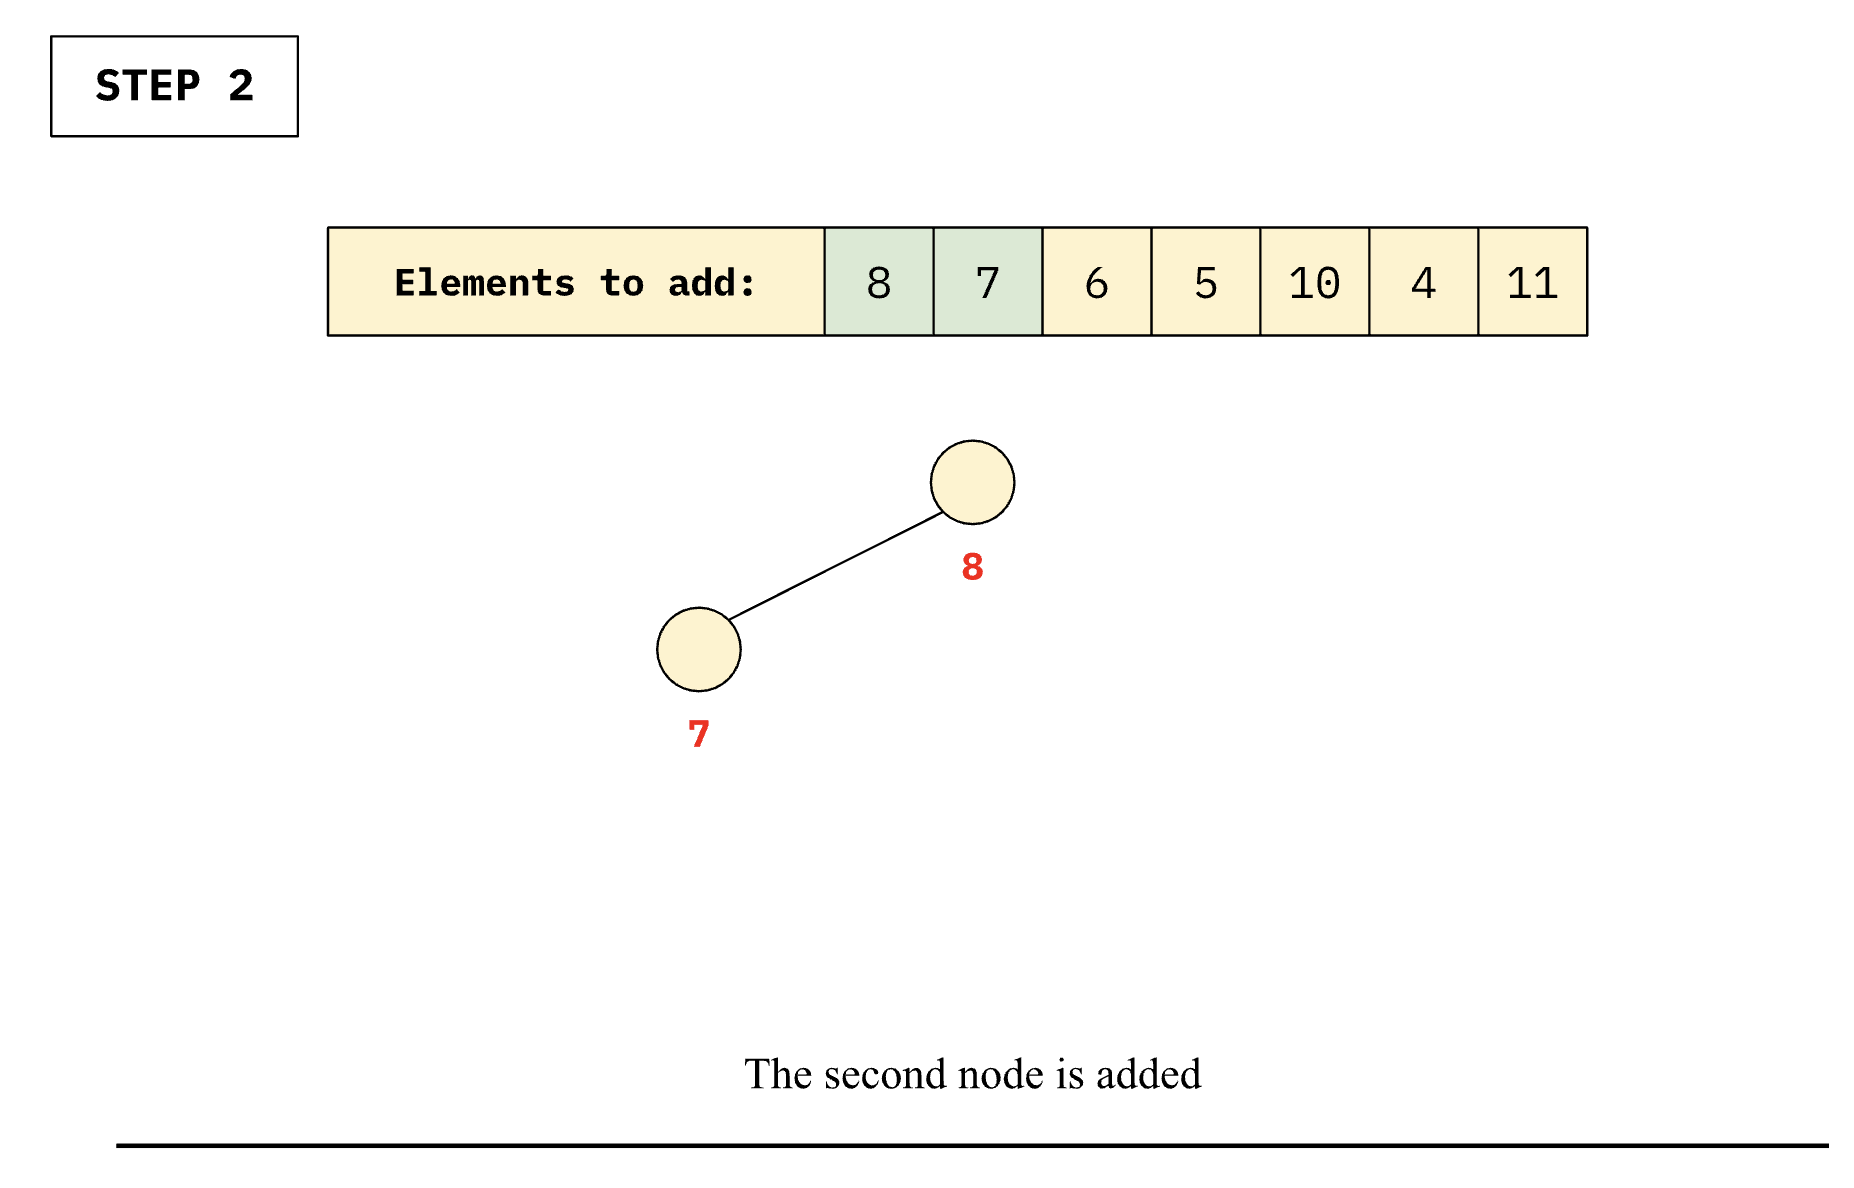
\includegraphics[width=0.8\linewidth]{Google Drawings/williams-2.png}
    \end{subfigure}
    \begin{subfigure}{\textwidth}
        \centering
        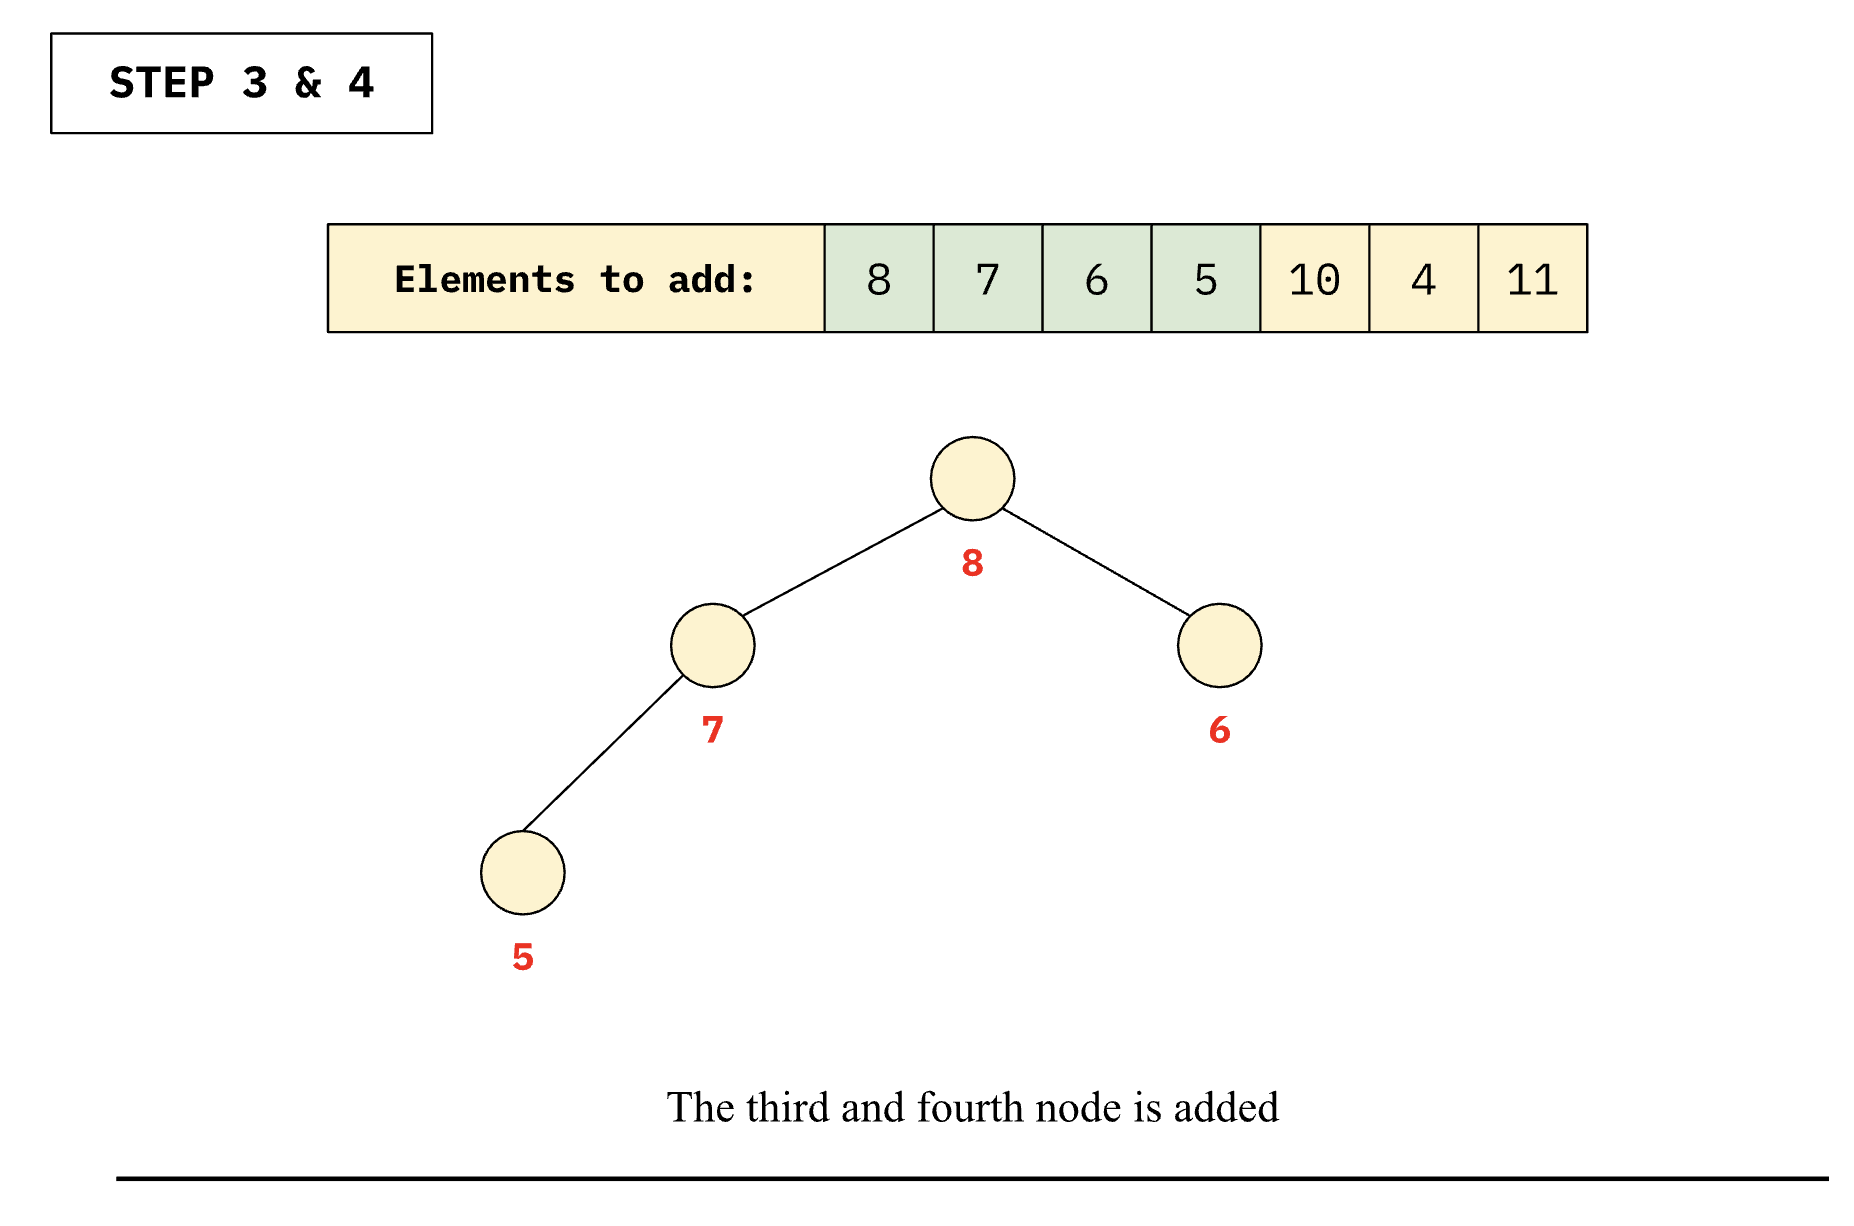
\includegraphics[width=0.8\linewidth]{Google Drawings/williams-3-4.png}
    \end{subfigure}
\end{figure}
\begin{figure}[H]
    \ContinuedFloat
    \begin{subfigure}{\textwidth}
        \centering
        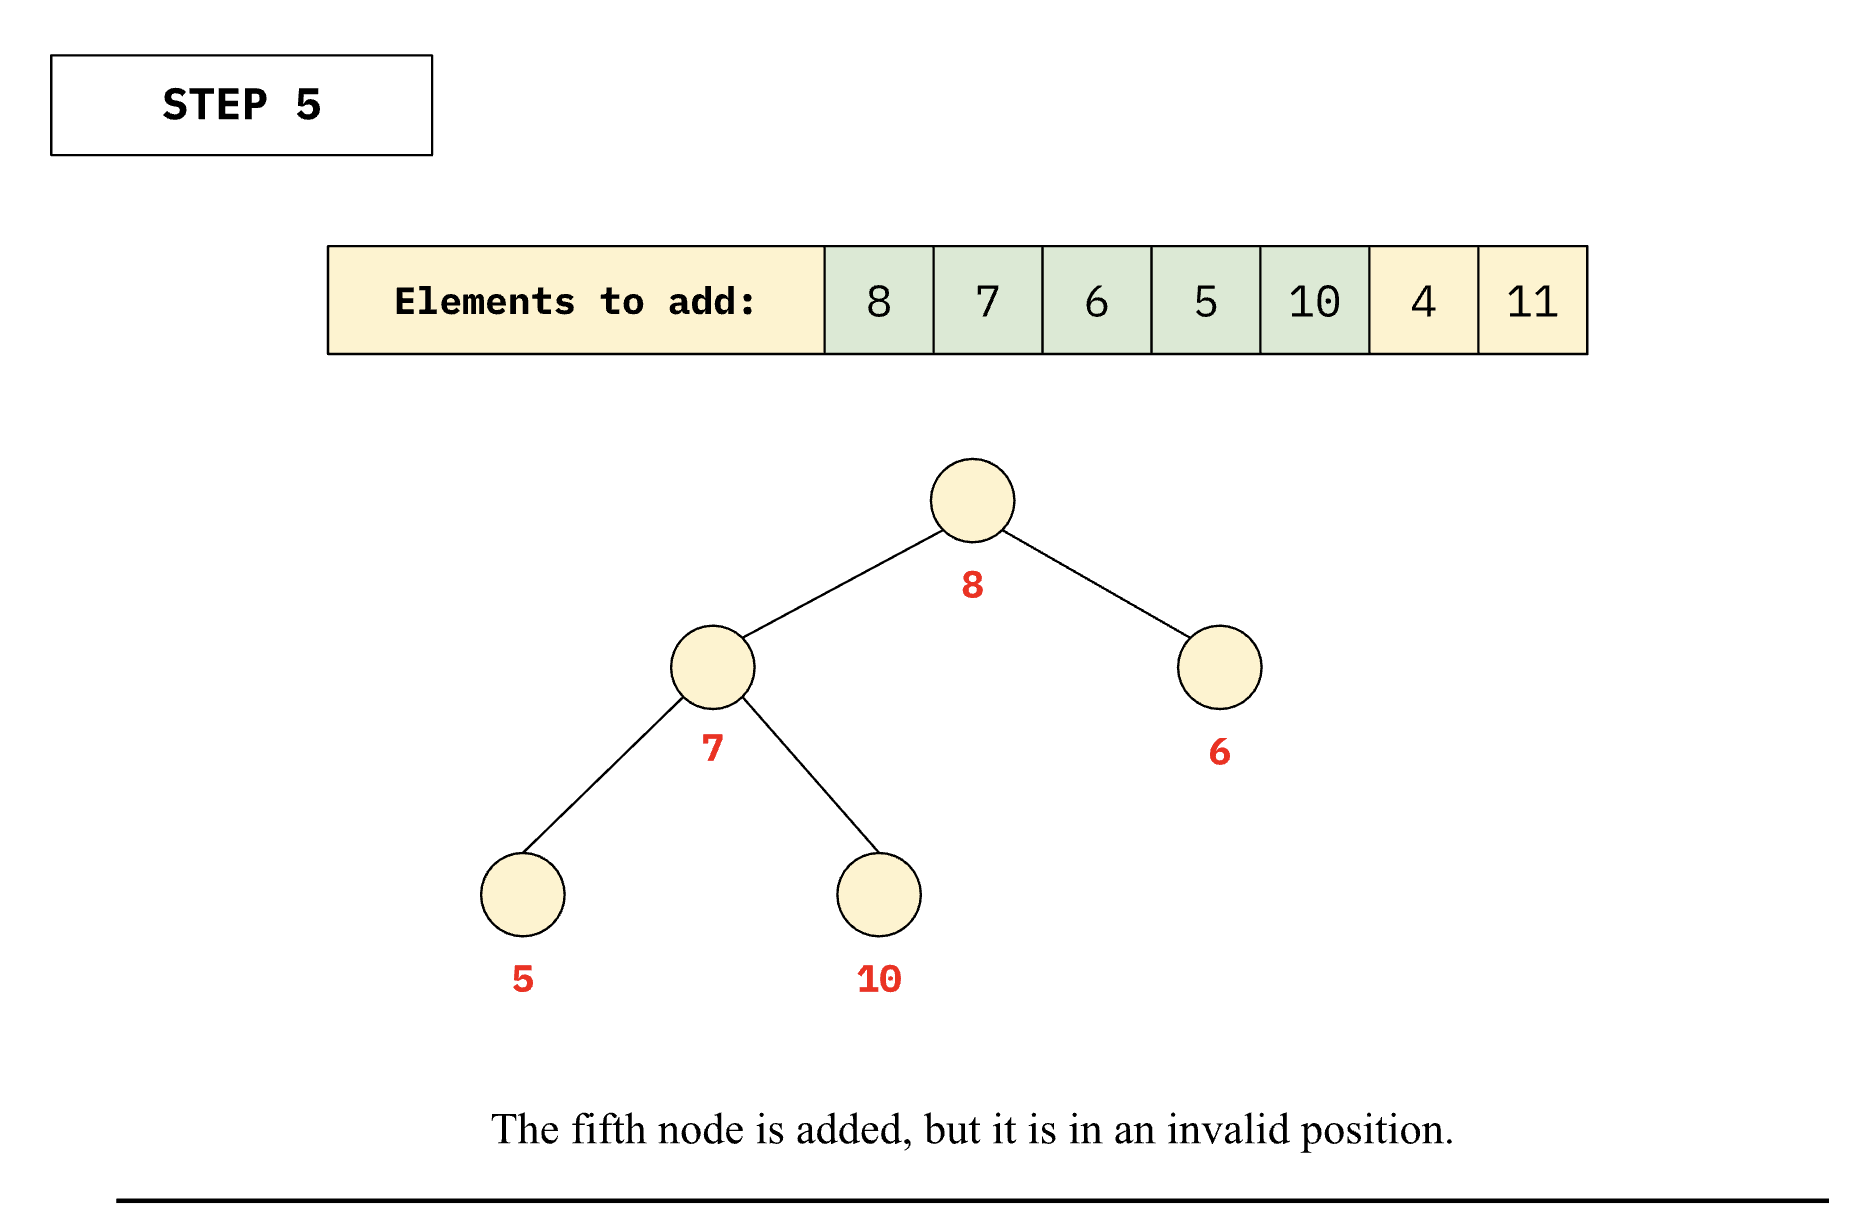
\includegraphics[width=0.8\linewidth]{Google Drawings/williams-5.png}
    \end{subfigure}
    \begin{subfigure}{\textwidth}
        \centering
        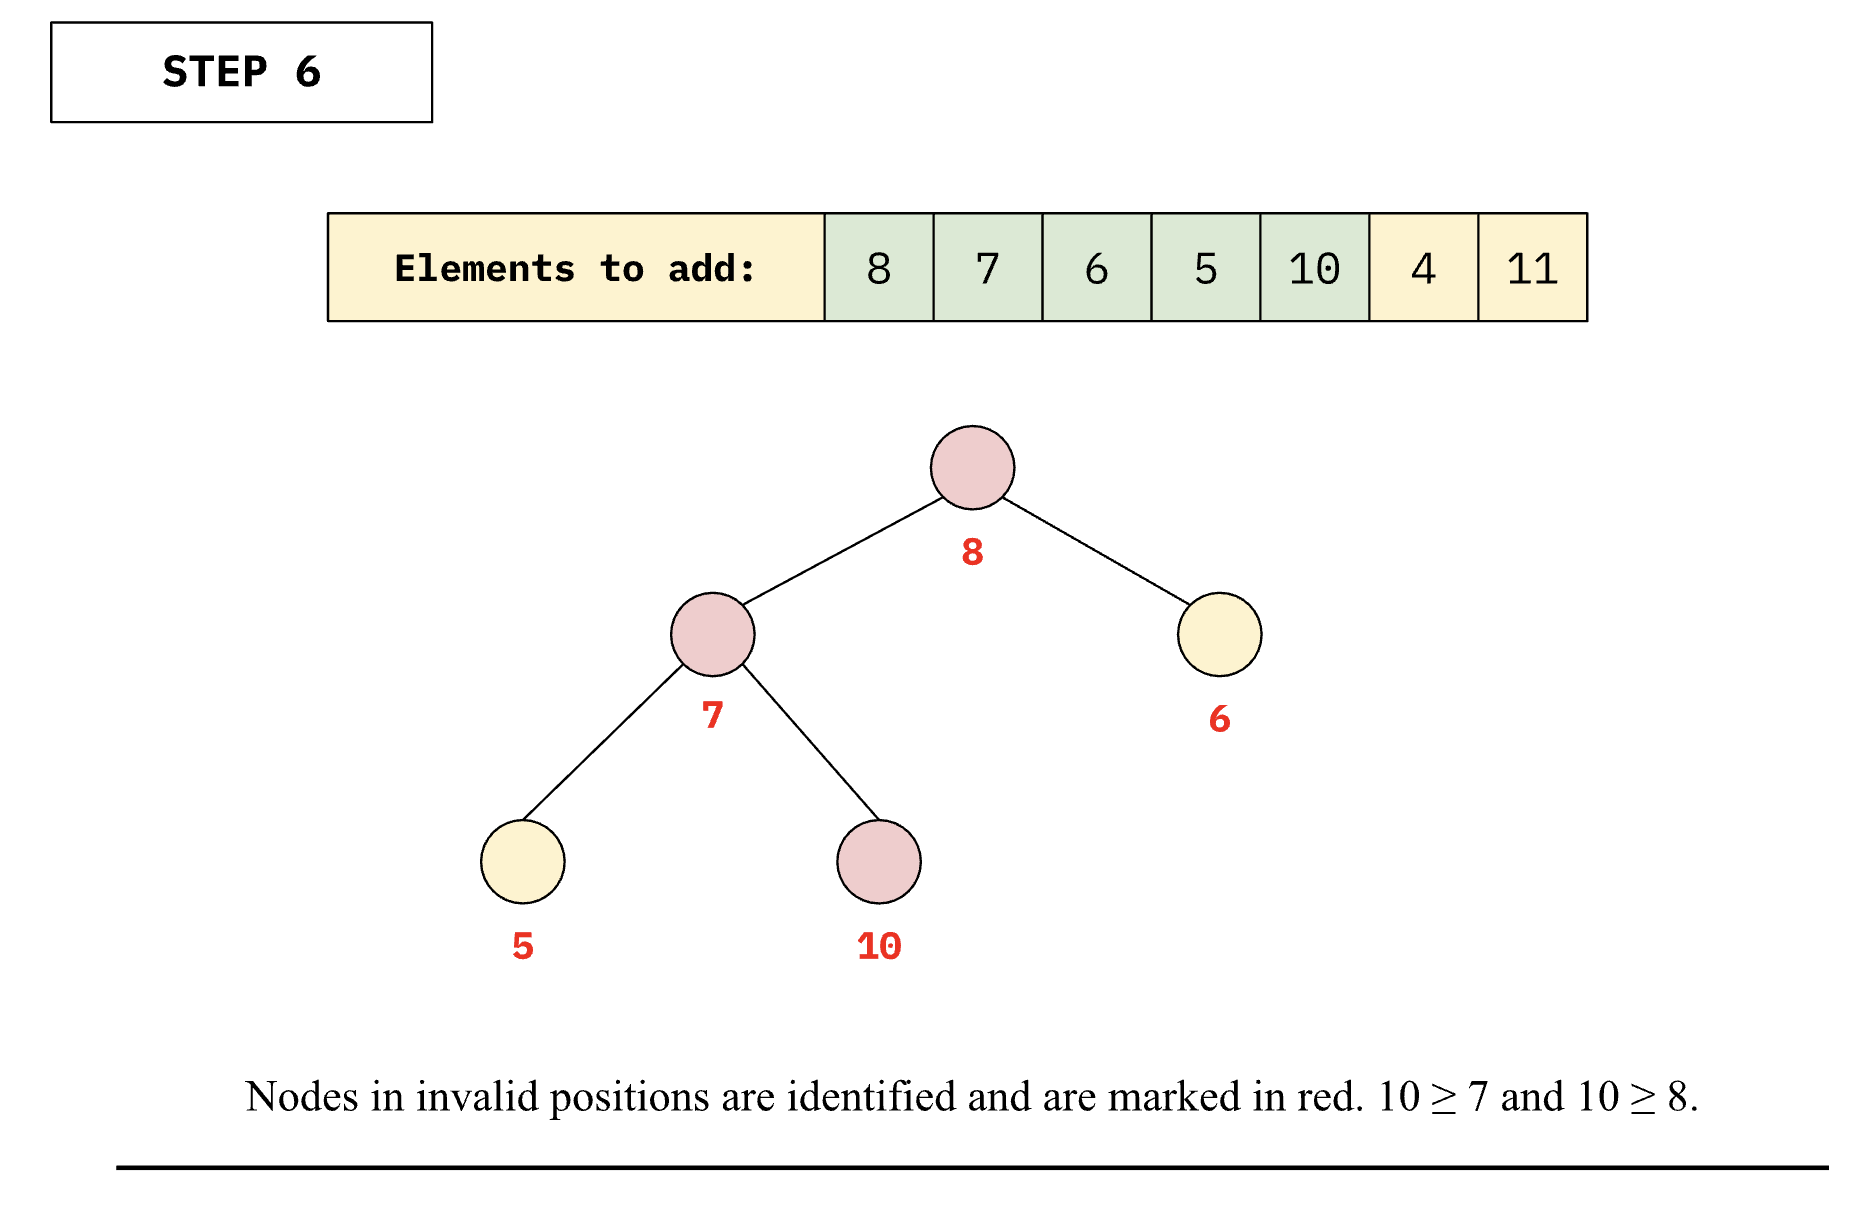
\includegraphics[width=0.8\linewidth]{Google Drawings/williams-6.png}
    \end{subfigure}
    \begin{subfigure}{\textwidth}
        \centering
        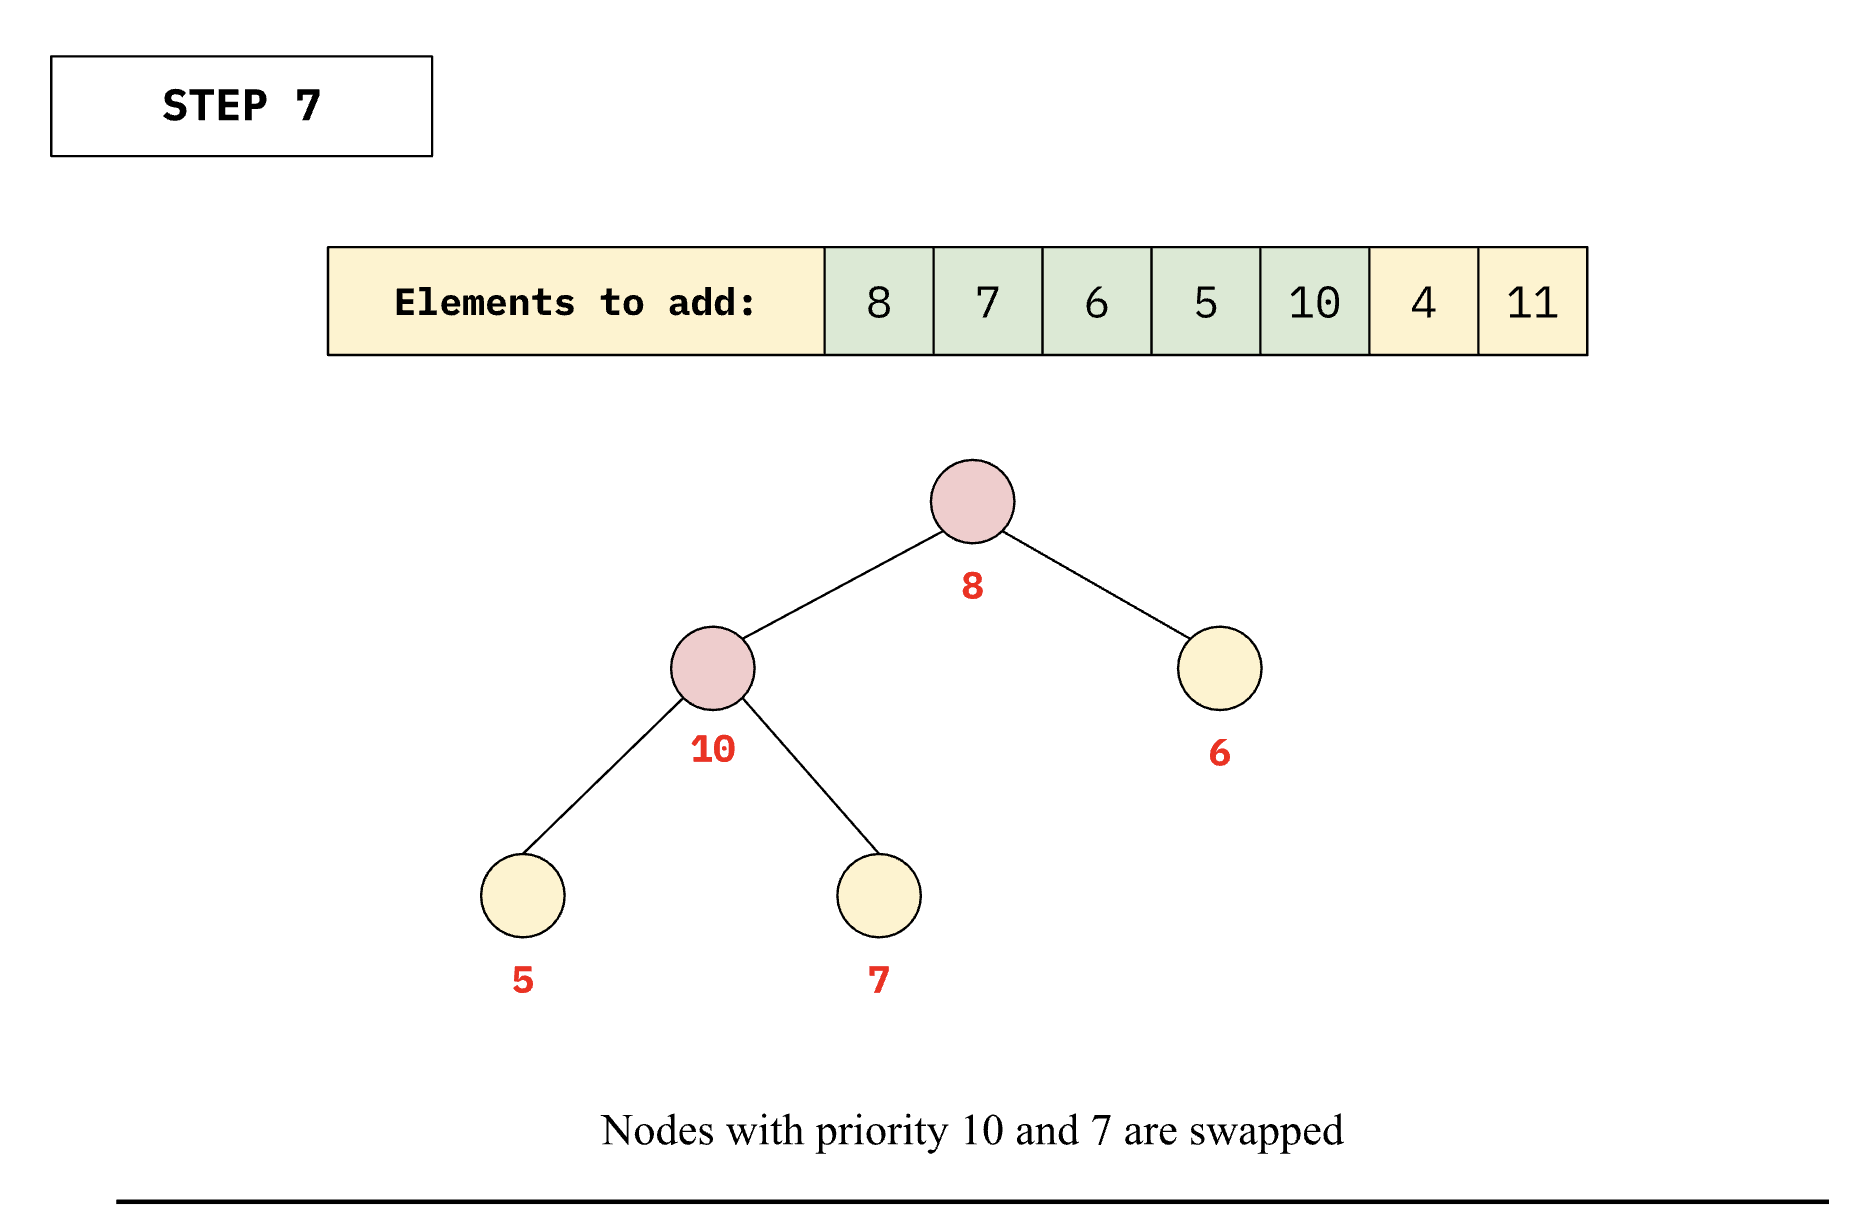
\includegraphics[width=0.8\linewidth]{Google Drawings/williams-7.png}
    \end{subfigure}
\end{figure}
\begin{figure}[H]
    \ContinuedFloat
    \begin{subfigure}{\textwidth}
        \centering
        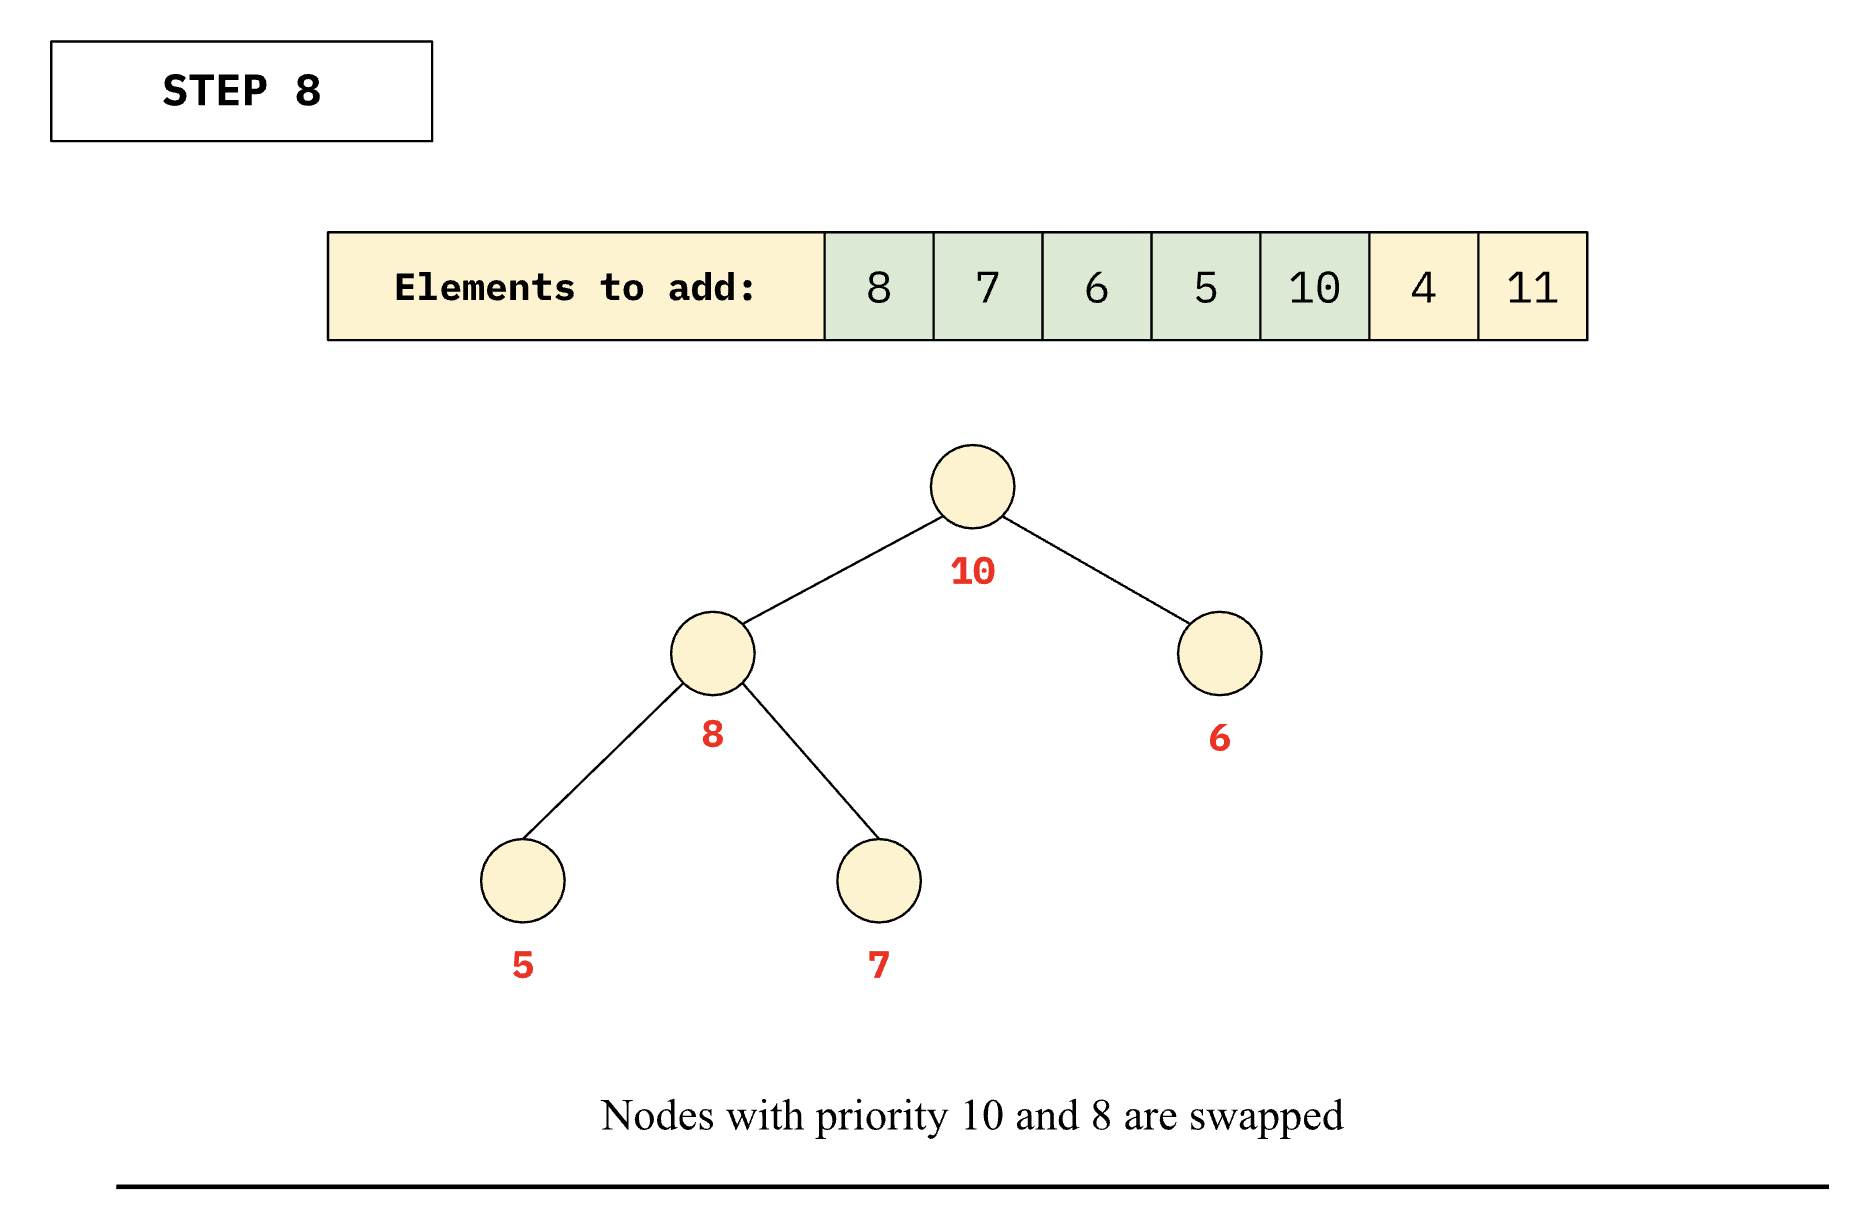
\includegraphics[width=0.8\linewidth]{Google Drawings/williams-8.png}
    \end{subfigure}
    \begin{subfigure}{\textwidth}
        \centering
        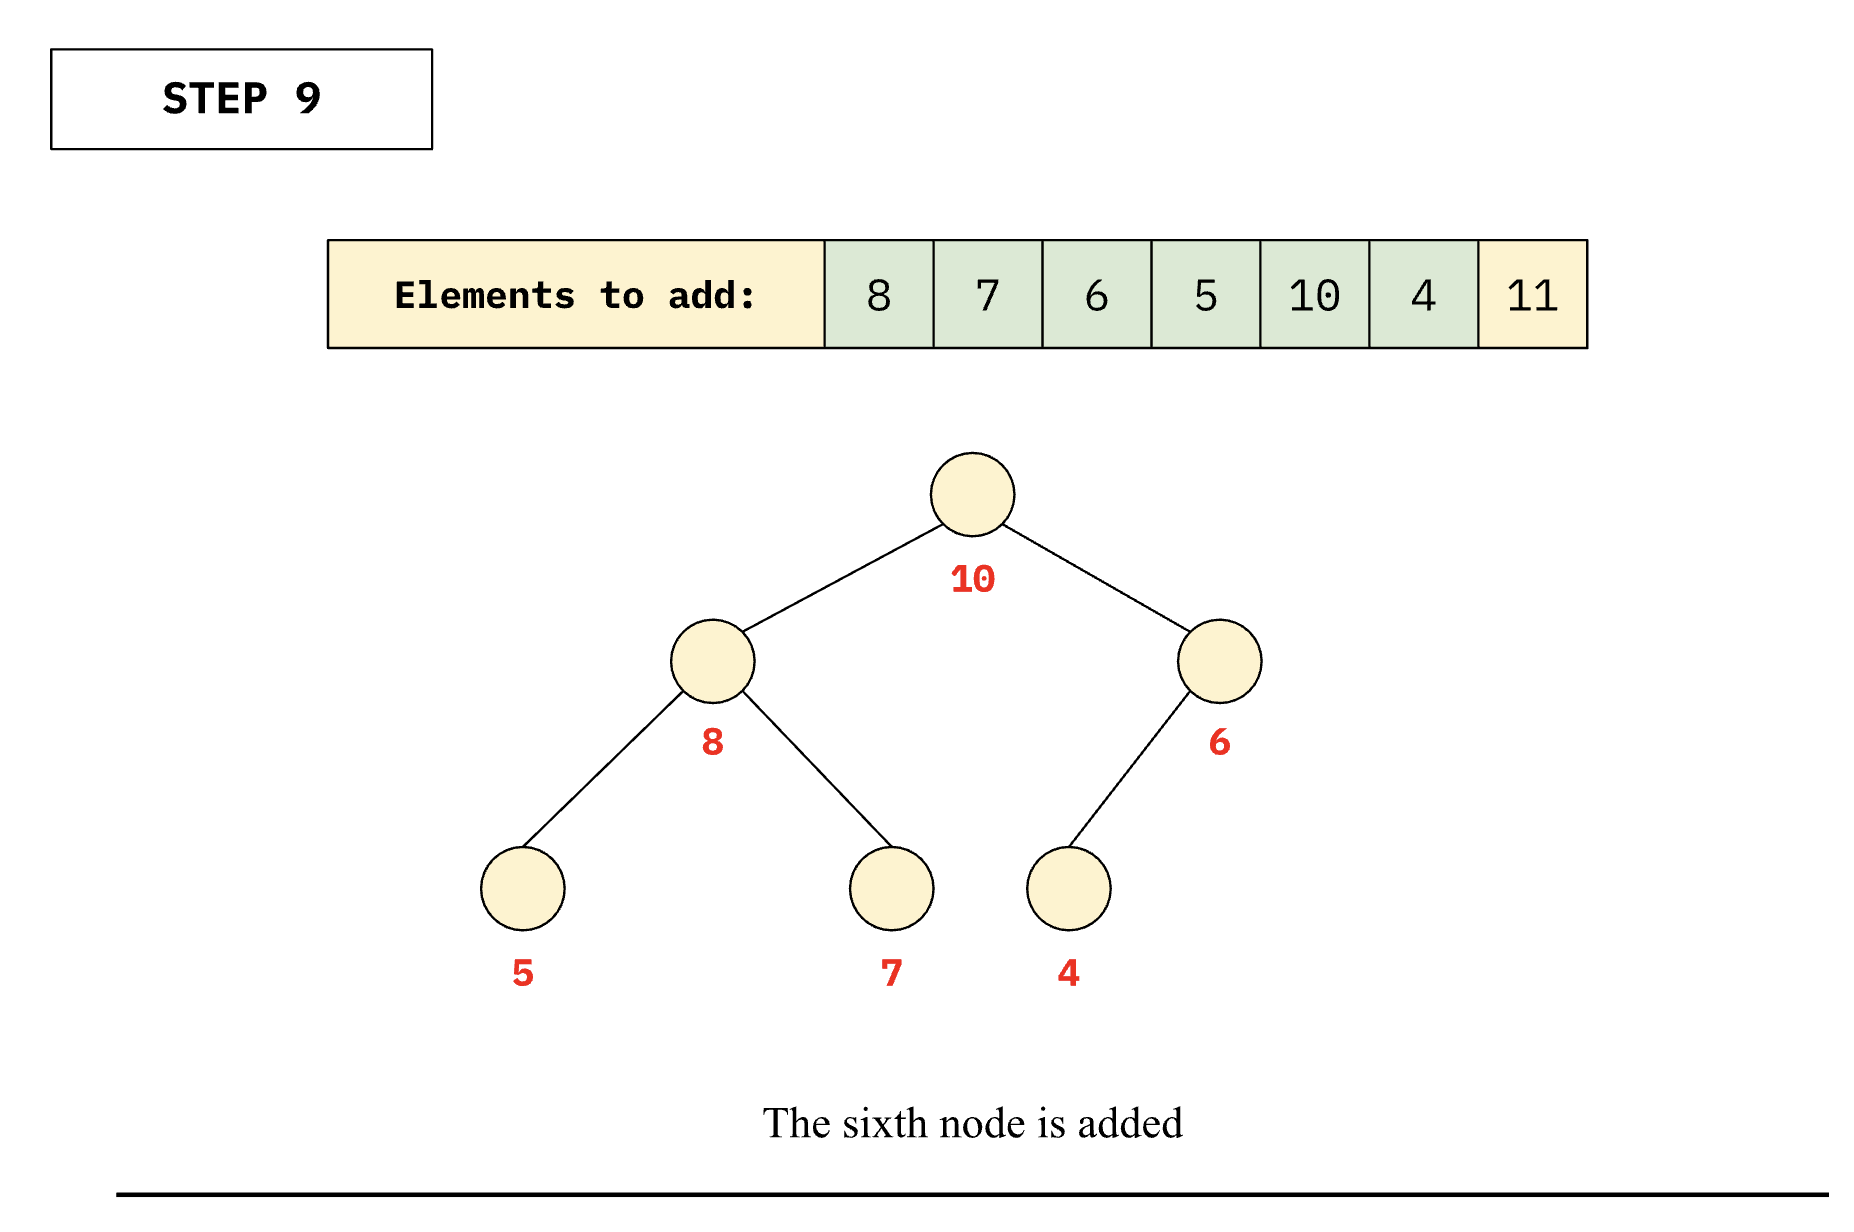
\includegraphics[width=0.8\linewidth]{Google Drawings/williams-9.png}
    \end{subfigure}
    \begin{subfigure}{\textwidth}
        \centering
        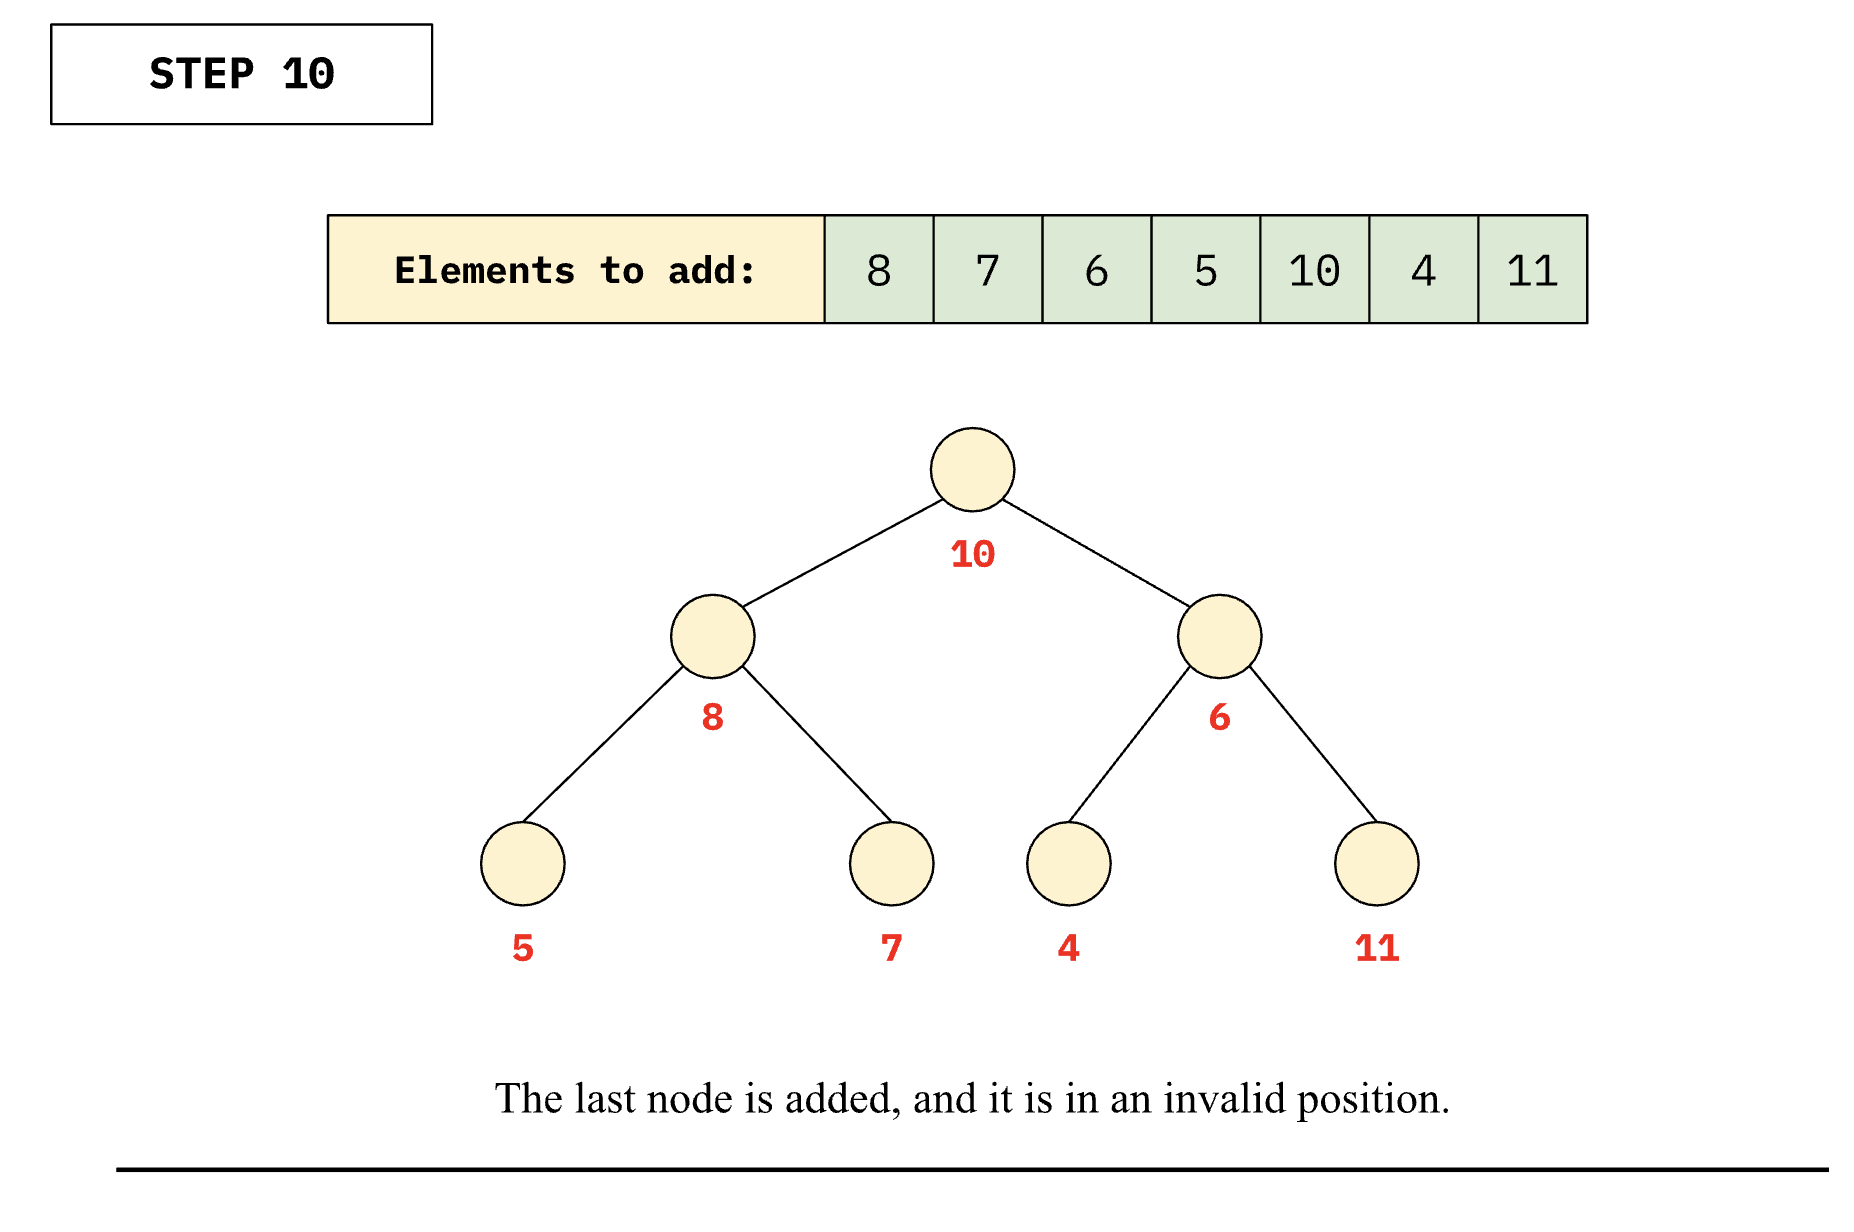
\includegraphics[width=0.8\linewidth]{Google Drawings/williams-10.png}
    \end{subfigure}
\end{figure}
\begin{figure}[H]
    \ContinuedFloat
    \begin{subfigure}{\textwidth}
        \centering
        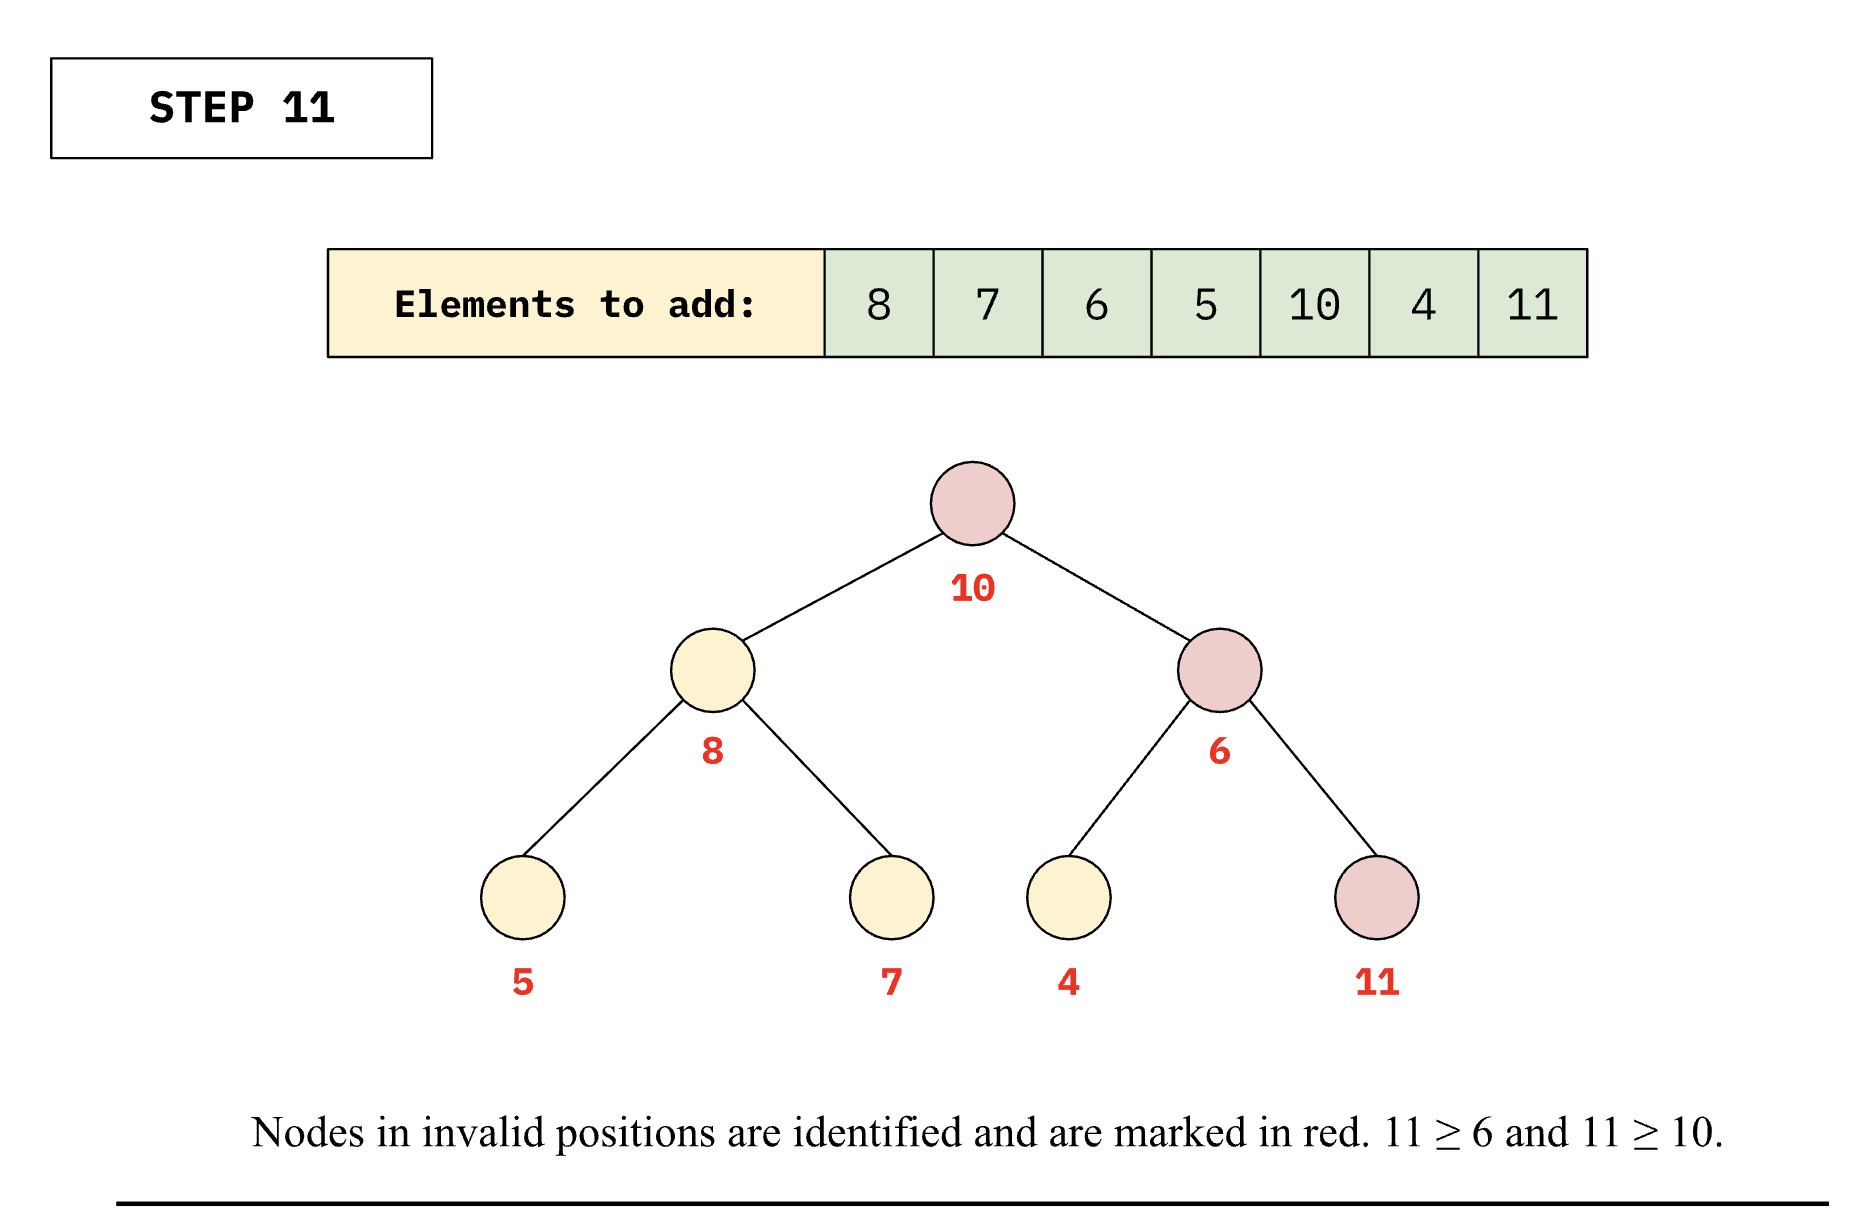
\includegraphics[width=0.8\linewidth]{Google Drawings/williams-11.png}
    \end{subfigure}
    \begin{subfigure}{\textwidth}
        \centering
        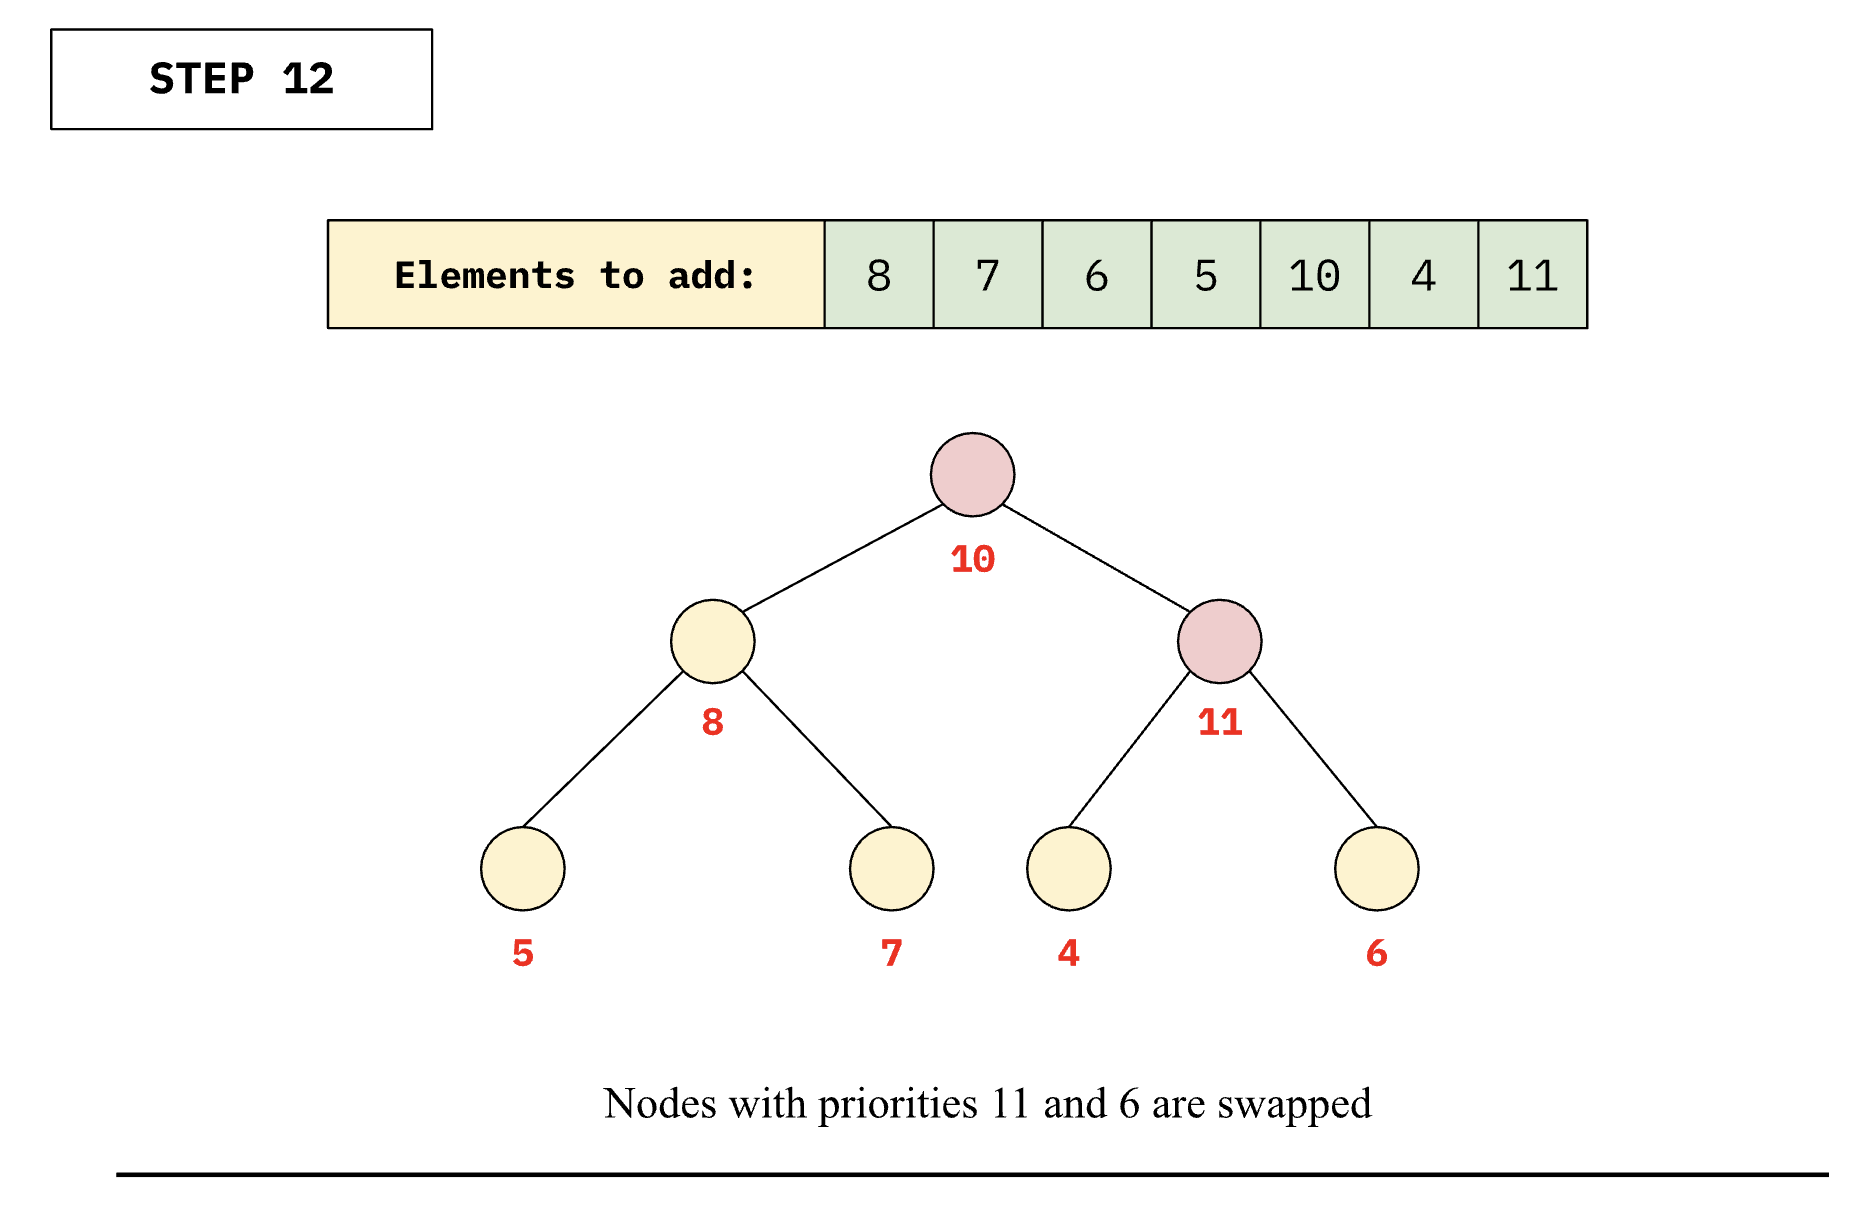
\includegraphics[width=0.8\linewidth]{Google Drawings/williams-12.png}
    \end{subfigure}
    \begin{subfigure}{\textwidth}
        \centering
        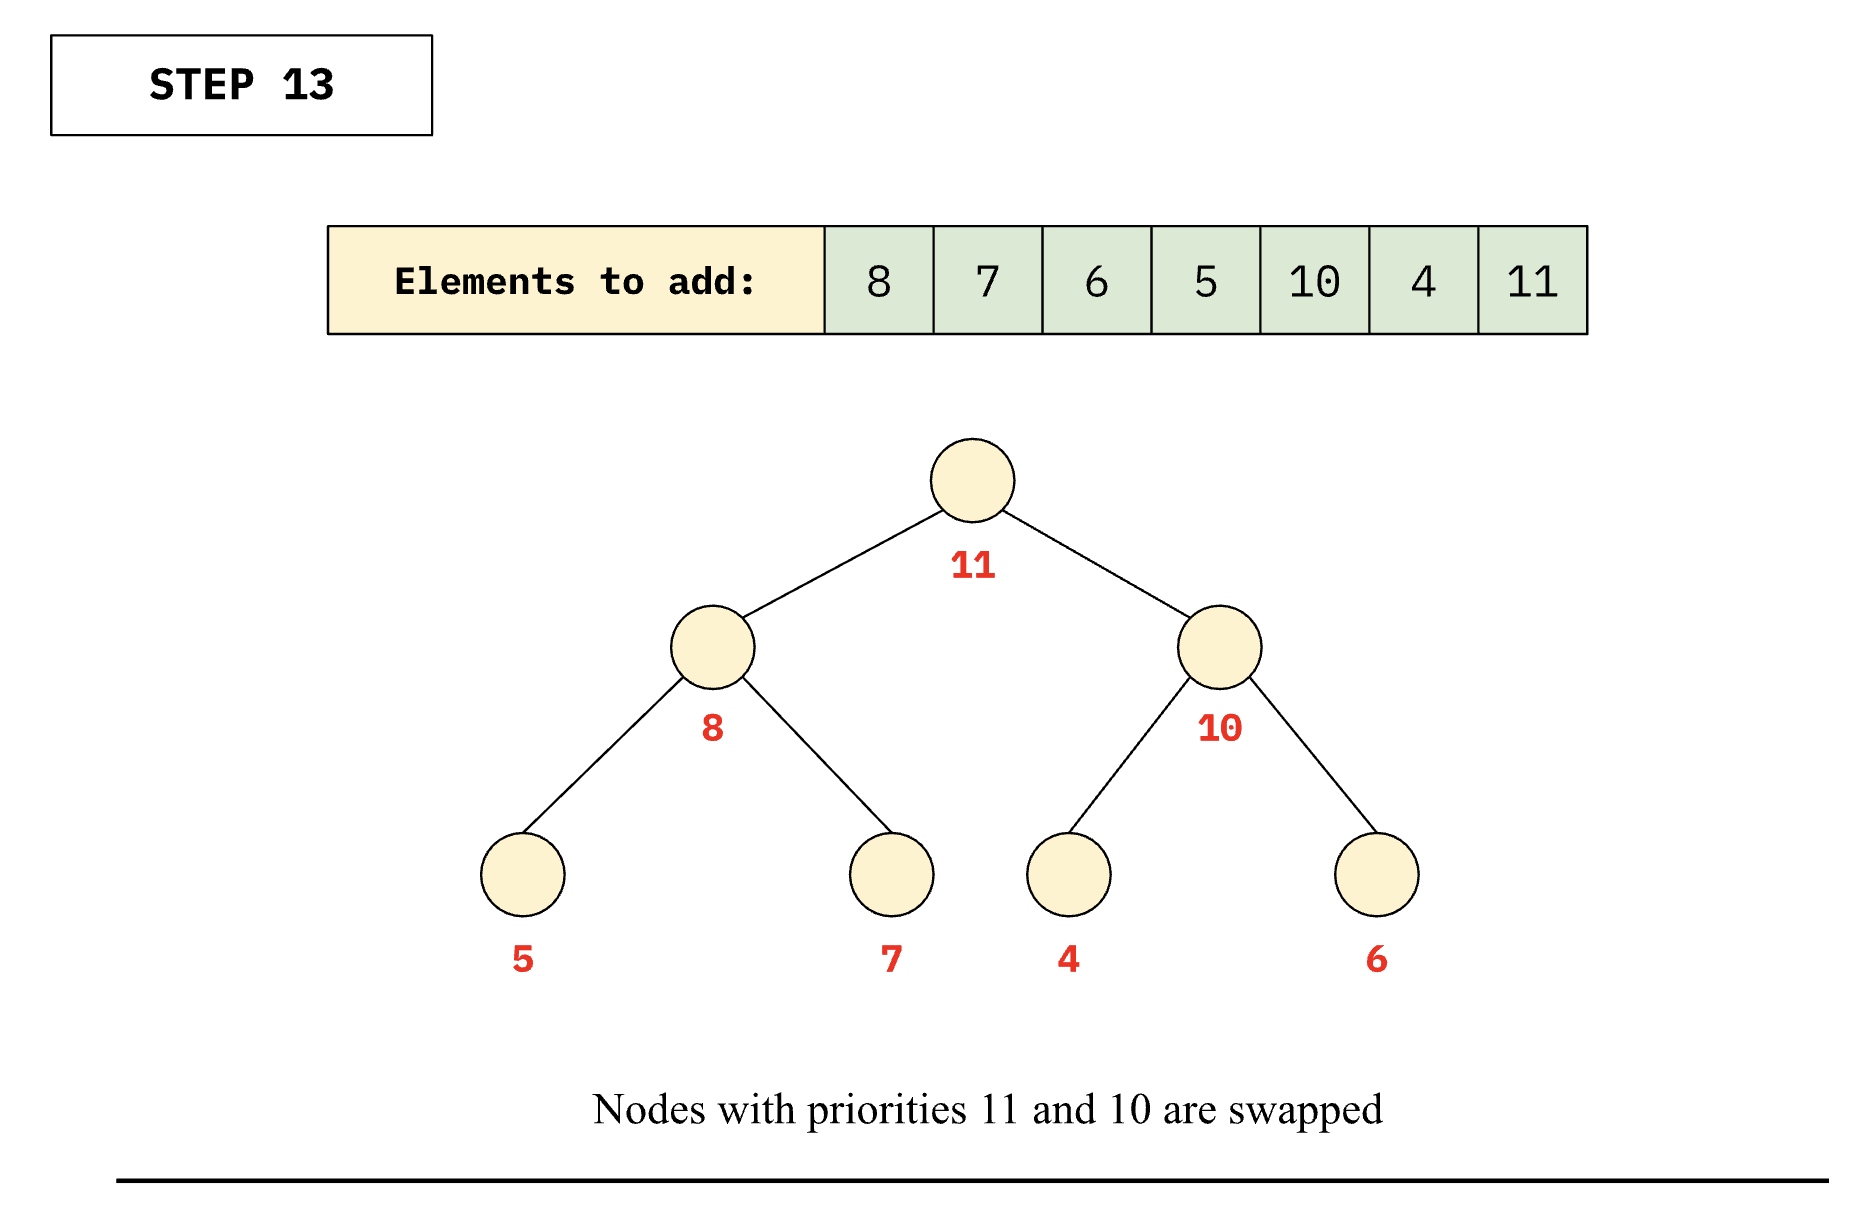
\includegraphics[width=0.8\linewidth]{Google Drawings/williams-13.png}
    \end{subfigure}
\end{figure}

In figure \ref{fig:williams-creation}, each element that was added had a priority that was lower than the one before it except in steps 5 and 10. This was to demonstrate how Williams's heap creation method swapped nodes that were added in an invalid position and how it did not swap the other nodes that were placed in valid positions.\newline

To describe the speed of Williams's method, I will assume a worst case scenario, where every new element added to the priority queue would be larger than all existing elements in the queue, requiring the rearrangement of nodes all the way up to the root node, as seen with the nodes with priorities $10$ and $11$ in figure \ref{fig:williams-creation}. Therefore, as the number of elements increases in a binary heap, the more swaps are needed to create a binary heap. This is explained in the following section.\newline

\subsection{Obtaining the OPS function}
Let $P(H)$ be the number of operations Williams’s heap creation method requires given height $H$. To find the OOG of the OPS function of Williams’s method, I would first need to find $O(P(H))$ and simplify it to be in terms of $N$.\newline

In table \ref{tab:ops-vs-nodes-williams}, the total number of operations at level $L$ in a binary heap as well as the total number of operations for a binary heap of height $H$ is shown.

\begin{table}[H]
    \centering
    \bgroup
    \singlespacing
    \caption{Table of total no. of operations compared to number of nodes}
    \small
    \renewcommand\tabularxcolumn[1]{m{#1}}
    \renewcommand{\arraystretch}{1.5}
    \begin{tabularx}{0.9\textwidth}{|X|c|c|c|c|c|c|c|c|c|}
    \hline
    \RaggedRight{$L$} & $0$ & $1$ & $2$ & $3$ & $4$ & $5$ & $6$ & \dots & $H$\\
    \hline
    \RaggedRight{No. of nodes at level $L$} & $2^0$ & $2^1$ & $2^2$ & $2^3$ & $2^4$ & $2^5$ & $2^6$ & \dots & $2^H$\\
    \hline
    \RaggedRight{No. of operations at level $L$} & $0$ & $2$ & $8$ & $24$ & $64$ & $160$ & $384$ & \dots & $2^H\times H$\\
    \hline
    \RaggedRight{Total no. of operations for a binary heap of height $L$}
    & $0$ & $2$ & $10$ & $34$ & $98$ & $258$ & $642$ & \dots & $P(H)$\\
    \hline
    \end{tabularx}
    \label{tab:ops-vs-nodes-williams}
    \egroup
\end{table}

I discovered that the total number of operations for a binary heap of \textbf{height} $H$ is an accumulation of the values of the total number of operations at \textbf{levels} less than or equal to $H$ in a binary heap. So, I was able to express $P(H)$ as a series, one term for each level.\vspace{-1em}

\bgroup
\onehalfspacing
\[P(0)=2^0\times 0=0\]
\[P(1)=(2^0\times 0)+(2^1\times 1)=2\]
\[P(2)=(2^0\times 0)+(2^1\times 1)+(2^2\times 2)=10\]
\[P(3)=(2^0\times0)+(2^1\times1)+(2^2\times2)+(2^3\times3)=34\]
\[\vdots\]
\[P(H)=\sum^H_{i=0}(2^i\times i)\]

\begin{center}
    This can also be expressed recursively as
\end{center}

\begin{equation*}
  P(H) =
    \begin{cases}
      0 & \text{if } H=0\\
      P(H-1)+2^H\times H & \text{if } H\geq1 \\
    \end{cases}       
\end{equation*}
\egroup
\vspace{0.5em}

% I realised that such a recursive expression is just like how cumulative frequency is calculated over a discrete variable which takes only integer values. If we let $f_x$ be the frequency of data points where the variable has a value of $x$, and $F_x$ be the cumulative frequency of data points where the variable has a value $\leq x$, $F_x=F_{x-1}+f_x=\sum^x_{i=0}(f_i)$.\newline

Unfortunately, simplifying $P(H)=\sum^H_{i=0}(2^i\times i)$ with just the sigma notation is difficult as the series is neither arithmetic nor geometric. Therefore, I decided to plot the relationship of $N$ to the total number of operations for binary heaps with heights $0$ to $6$.\newline

Let $Q(N) \equiv P(H)$ be the equivalent function that provides the OPS function of Williams's method, in a binary heap.

\begin{figure}[H]
    \centering
    \caption{Graphed relationship between $N$ and $Q(N)$}
    \includegraphics[width=0.75\linewidth]{Google Drawings/graph-N-and-qN.png}
    \label{fig:N-and-Q(N)-williams}
\end{figure}

In the figure above, $y=Q(N)$ is plotted as a black curve, using points that are marked. The OOG of $Q(N)$ seems to be $O(N^2)$ or less, but it is definitely greater than $O(N)$ as there is an increasing gradient. Since this finding did not present a coherent indication of the OOG of $Q(N)$, I decided to utilise upper and lower bounds of $Q(N)$ to narrow down its OOG, demonstrated in the following sections.

\subsection{Finding the upper bound}
I will define the upper bound of $Q(N)$ as $A(N)$, where $O(A(N))$ is less than $O(N^2)$ but greater than or equal to $O(Q(N))$.\newline

In figure \ref{fig:swaps-vs-height-williams}, it is shown that each node that is inserted is not always swapped the same amount of times as other nodes that are inserted, even in a worst case scenario, since the maximum number of swaps that can happen is decided by the level at which the node was added at. 
\vspace{10pt}
\begin{figure}[H]
    \centering
    \caption{Difference in swaps as height increases}
    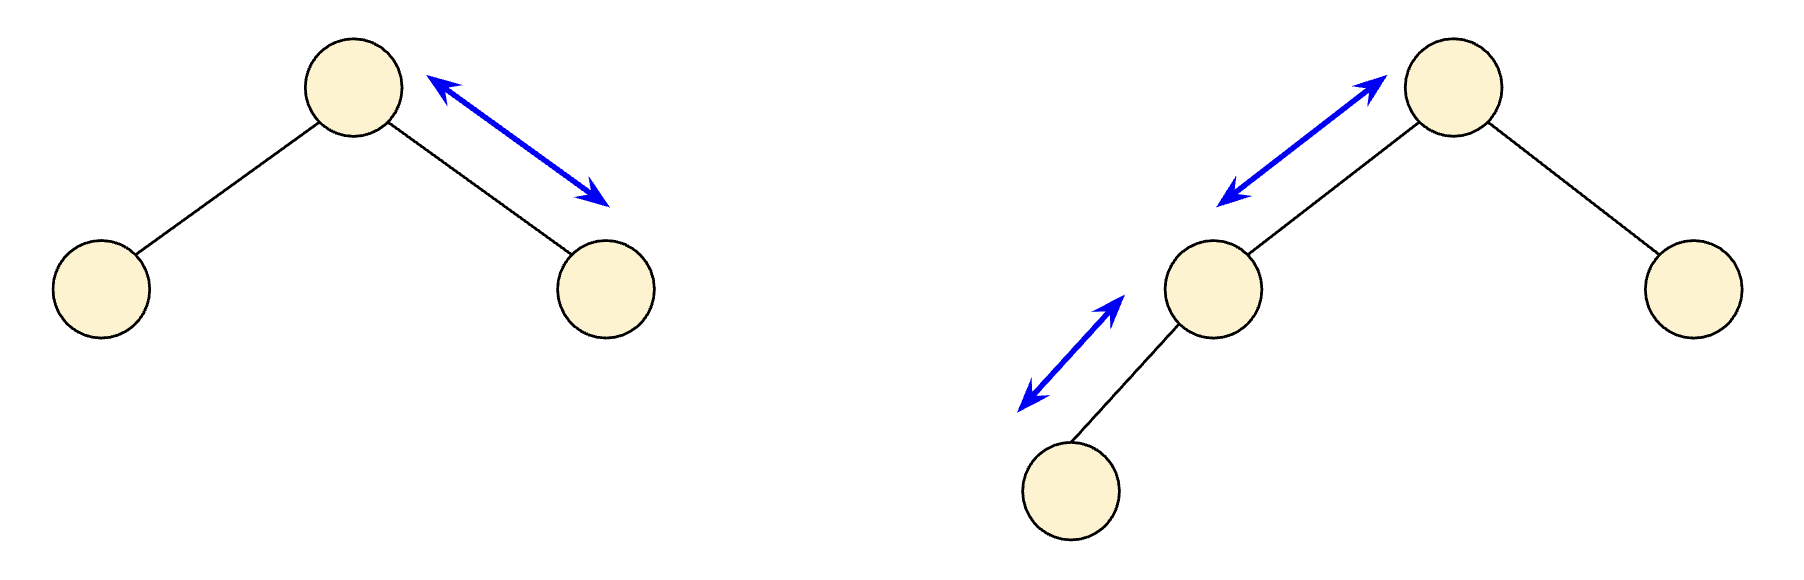
\includegraphics[width=0.75\linewidth]{Google Drawings/diff-in-swaps-height-increase.png}
    \label{fig:swaps-vs-height-williams}
\end{figure}

This is why $P(H)=\sum^H_{i=0}(2^i\times i)$ is difficult to calculate; there are variables in both the power and base of each term. If we over-estimate by assuming all nodes that are added are always swapped $H$ amount of times, we would have a total of $N\times H$ operations.
\vspace{-2em}

\bgroup
\onehalfspacing
\allowdisplaybreaks
\begin{align*}
    \text{Recall \eqref{eqn:H_ito_N},}\quad H&=\log_2(N+1)-1\\
    \text{Actual maximum operations }Q(N)&\leq N\times H\\
    &=N\times (\log_2(N+1)-1)\\
    &=N\log_2(N+1)-N\\
    &<N\log_2(N+1)\\
    &<N\log_2(N^2)\quad\text{ for large values of } N\\
    &=2N\log_2(N)=\text{upper bound of operations }A(N)\\
    &\in O(N\log(N))
\end{align*}
\egroup

Using inequalities, a loose upper bound, $A(N)$, was obtained with an OOG of $O(N\log (N))$. By definition of $O$-notation, the actual OOG of $Q(N)$ could either be $O(N\log (N))$, or less. To find it, I would have to obtain a lower bound for $Q(N)$ that is stricter with an OOG of $O(N \log(N))$, in order to form a tight bound for $Q(N)$.

\subsection{Finding the lower bound}
To obtain our lower bound, $B(N)$, I will underestimate the OPS function of Williams's method where it would be impossibly small as compared to  the actual maximum operations, $Q(N)$. This is done by assuming that only the nodes on the last level of the binary heap would be allowed to swap.\newline

\begin{figure}[H]
    \centering
    \caption{Example scenario of the lower bound of $Q(N)$}
    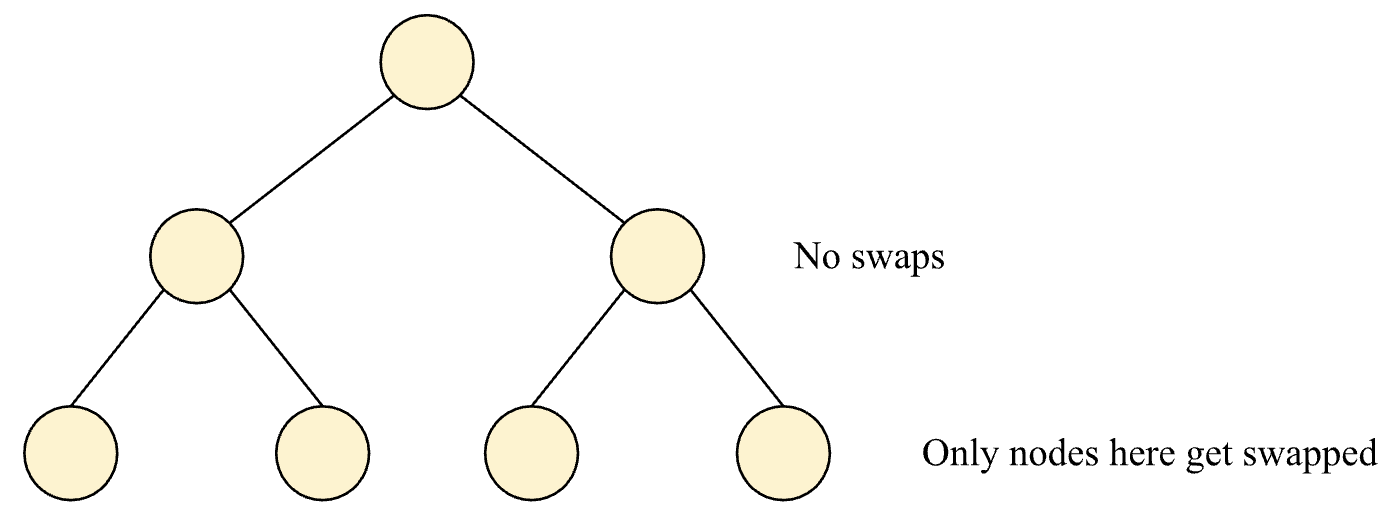
\includegraphics[width=0.75\linewidth]{Google Drawings/lower-bound-williams.png}
    \label{fig:example-lower-bounds-williams}
\end{figure}

As seen in figure \ref{fig:example-lower-bounds-williams}, for all binary heaps, each node on the last level of the binary heap will be swapped until the root node, assuming a worst case scenario. This gives us our lower bound, $2^H\times H$.
\vspace{-2em}

\bgroup
\onehalfspacing
\allowdisplaybreaks
\begin{align*}
    \text{Actual maximum operations }Q(N)&\geq2^H\times H\\
    &=2^{\log_2(N+1)-1}\times (\log_2(N+1)-1)\\
    &=\frac{2^{log_2(N+1)}}{2}\times (\log_2(N+1)-1)\\
    &=\frac{N+1}{2}\times (\log_2(N+1)-1)\\
    &>\frac{N}{2}\times (\log_2(N)-1)\\
    &=\frac{N}{2}\times (\log_2(N)-\log_2(2))\\
    &=\frac{N}{2}\times \log_2(\frac{N}{2})\\
    &>\frac{N}{2}\times \log_2(\sqrt{N})\quad\text{ for large values of } N\\
    &=\frac{N}{2}\times \log_2(N^{\frac{1}{2}})\\
    &=\frac{N}{4}\times \log_2(N)\\
    &=\text{lower bound of operations }B(N)
\end{align*}
\egroup

Hence, we get $A(N)=2N\log_2(N)$ as our loose upper bound and $B(N)=\frac{N}{4}\log_2(N)$ as our loose lower bound; I can now find the OOG of $Q(N)$.

\subsection{Obtaining the OOG}\label{williams_OOG}
Although $A(N)$ applies when $N\geq 3$ and $B(N)$ applies when $N\geq8$, this is acceptable since the OOG is calculated with large values of $N$. Because $Q(N)$ is exclusively between $A(N)$ and $B(N)$, which are made up of $N\log_2(N)$ multiplied by some positive constant, $Q(N)$, the OPS function of Williams's method, would have an OOG of $O(N\log(N))$.\newline

After the invention of Williams's method, computer scientist R. W. Floyd found a faster way of creating a binary heap, which has an OPS function with a lower OOG than Williams’s method \parencite[58]{JCC}.

\section{Floyd's binary heap creation method}
The process of creating a binary heap with Floyd’s method is shown through a step-by-step approach in figure \ref{fig:floyd-creation}.

\begin{figure}[H]
    \centering
    \caption{Creation of a binary heap with Floyd’s method}
    \label{fig:floyd-creation}
    \begin{subfigure}{\textwidth}
        \centering
        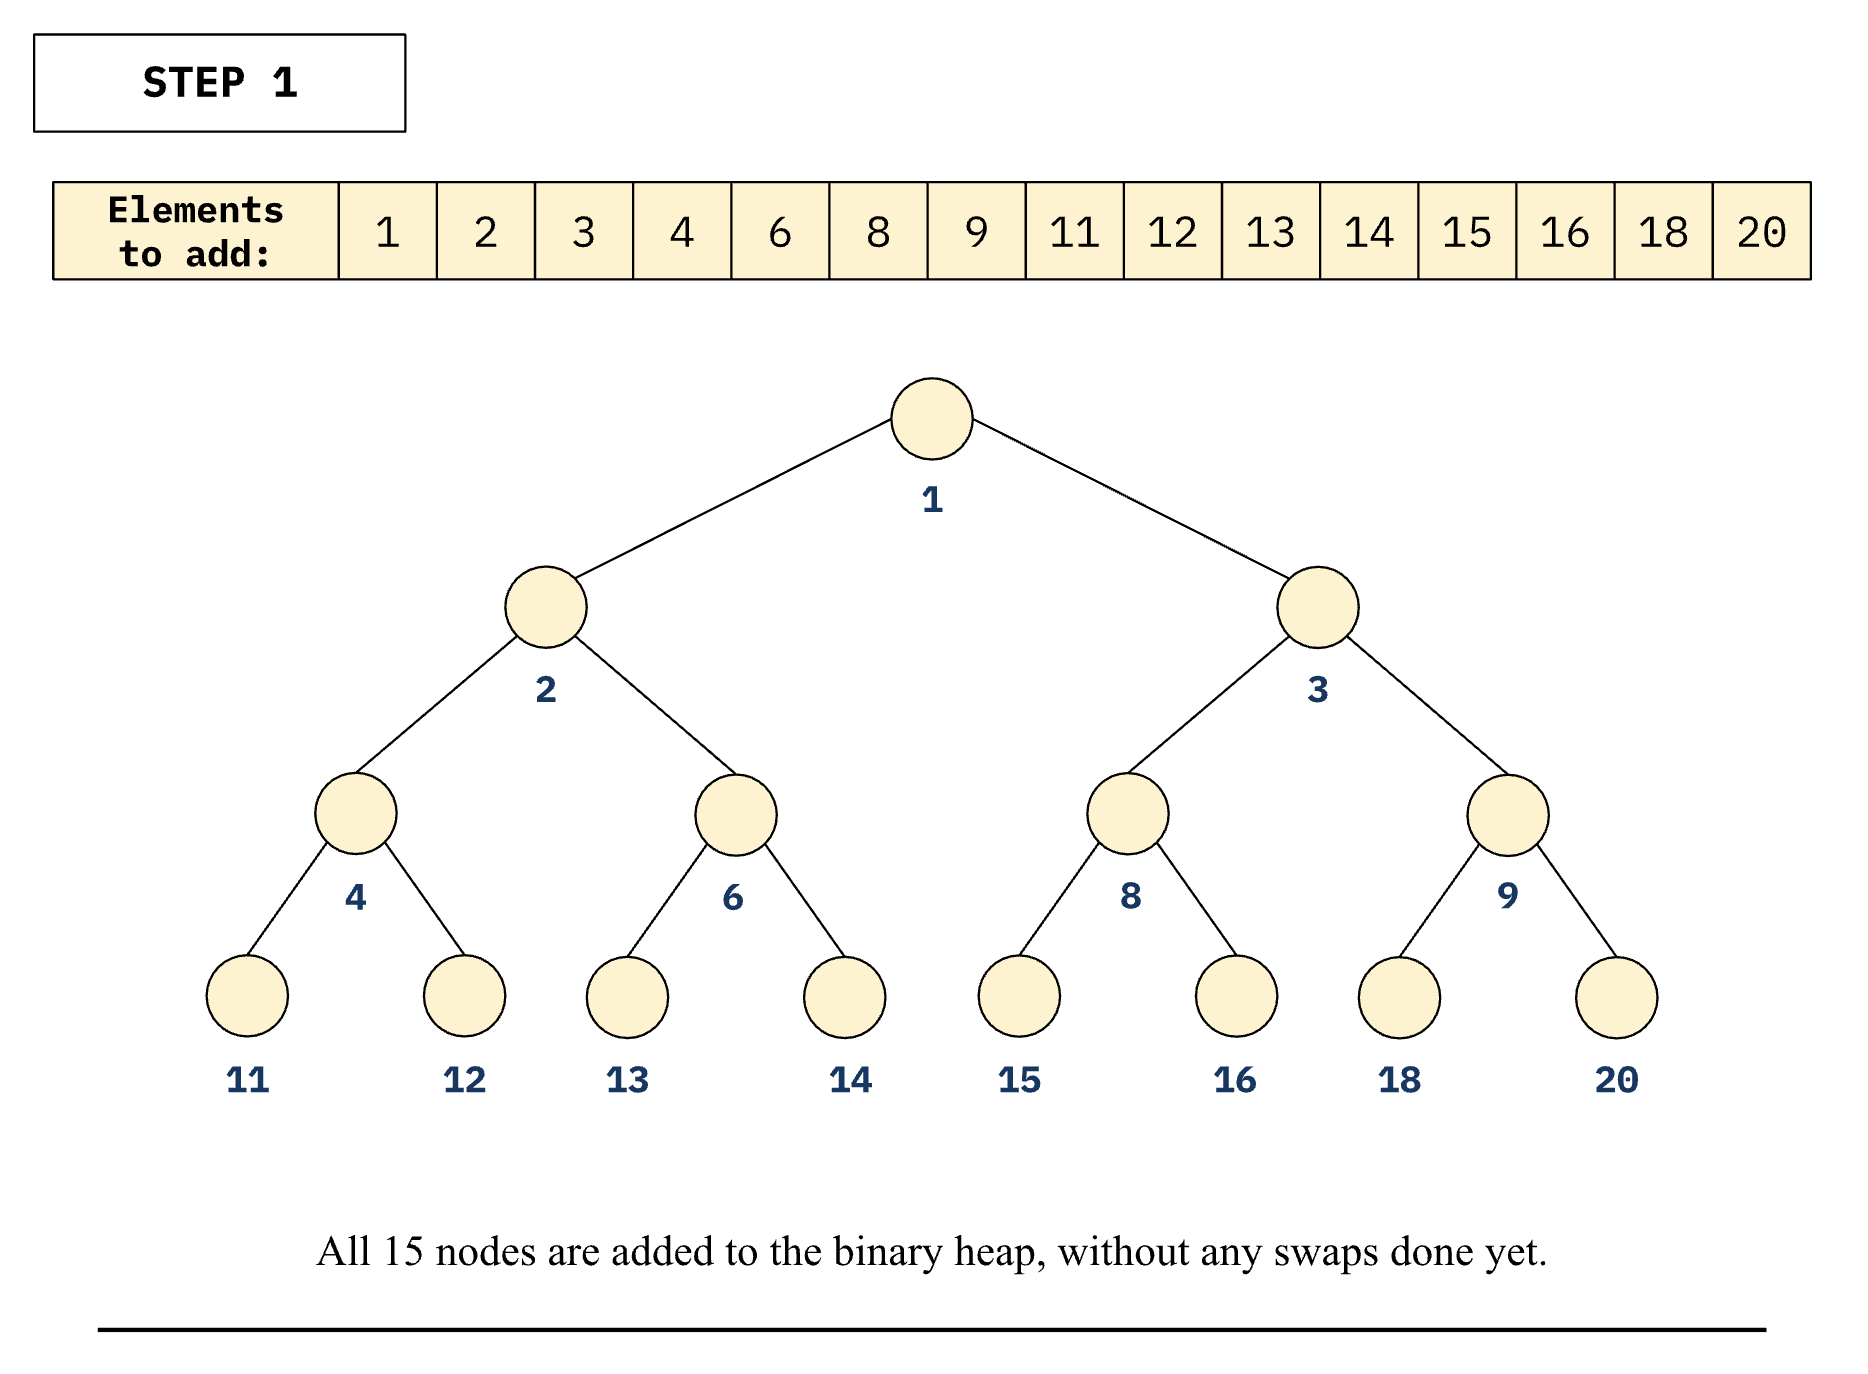
\includegraphics[width=0.72\linewidth]{Google Drawings/floyd-1.png}
    \end{subfigure}
    \begin{subfigure}{\textwidth}
        \centering
        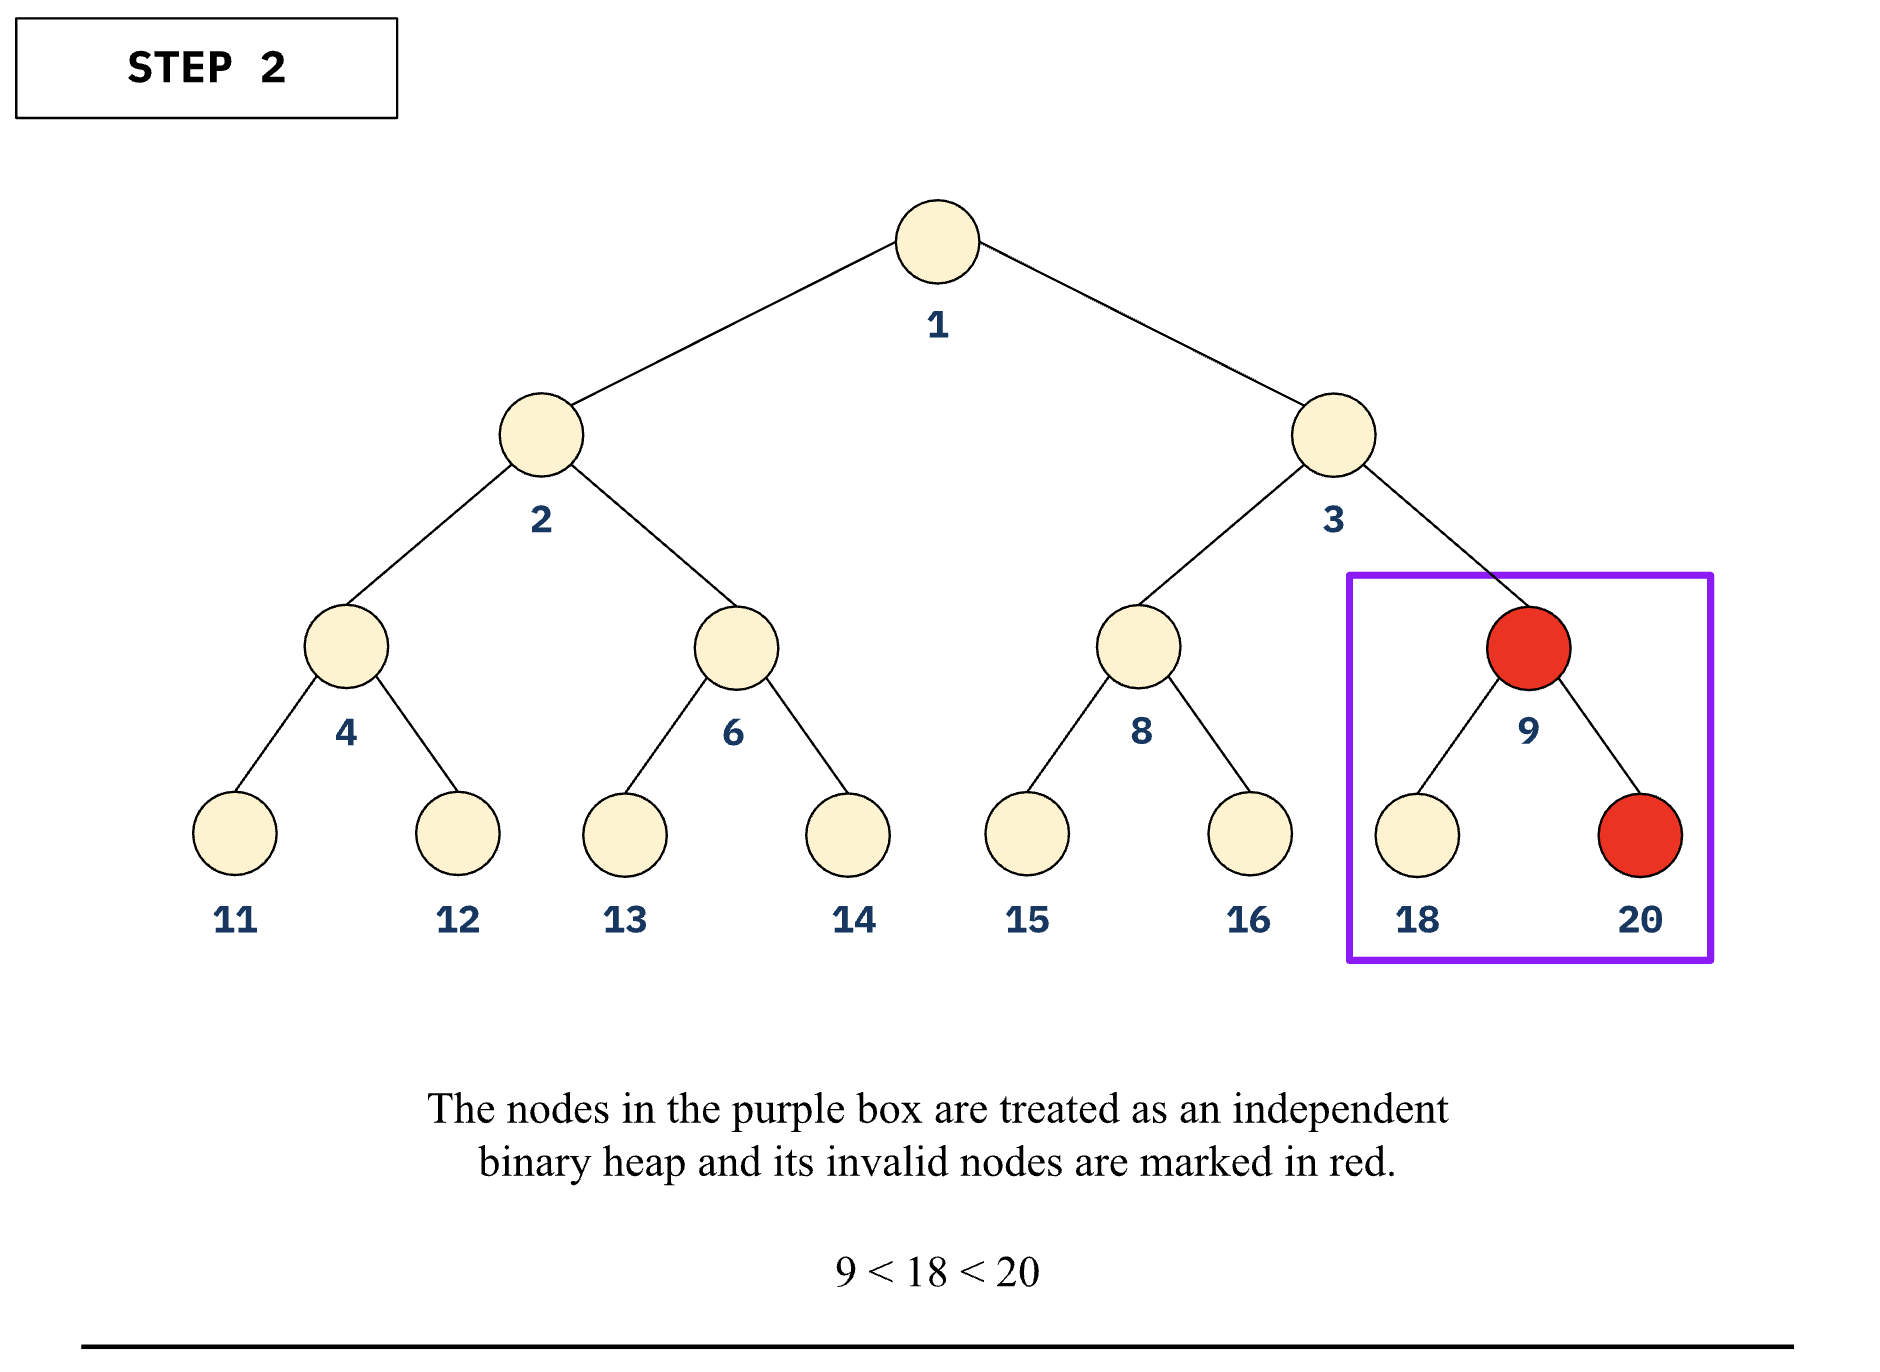
\includegraphics[width=0.72\linewidth]{Google Drawings/floyd-2.png}
    \end{subfigure}
    \begin{subfigure}{\textwidth}
        \centering
        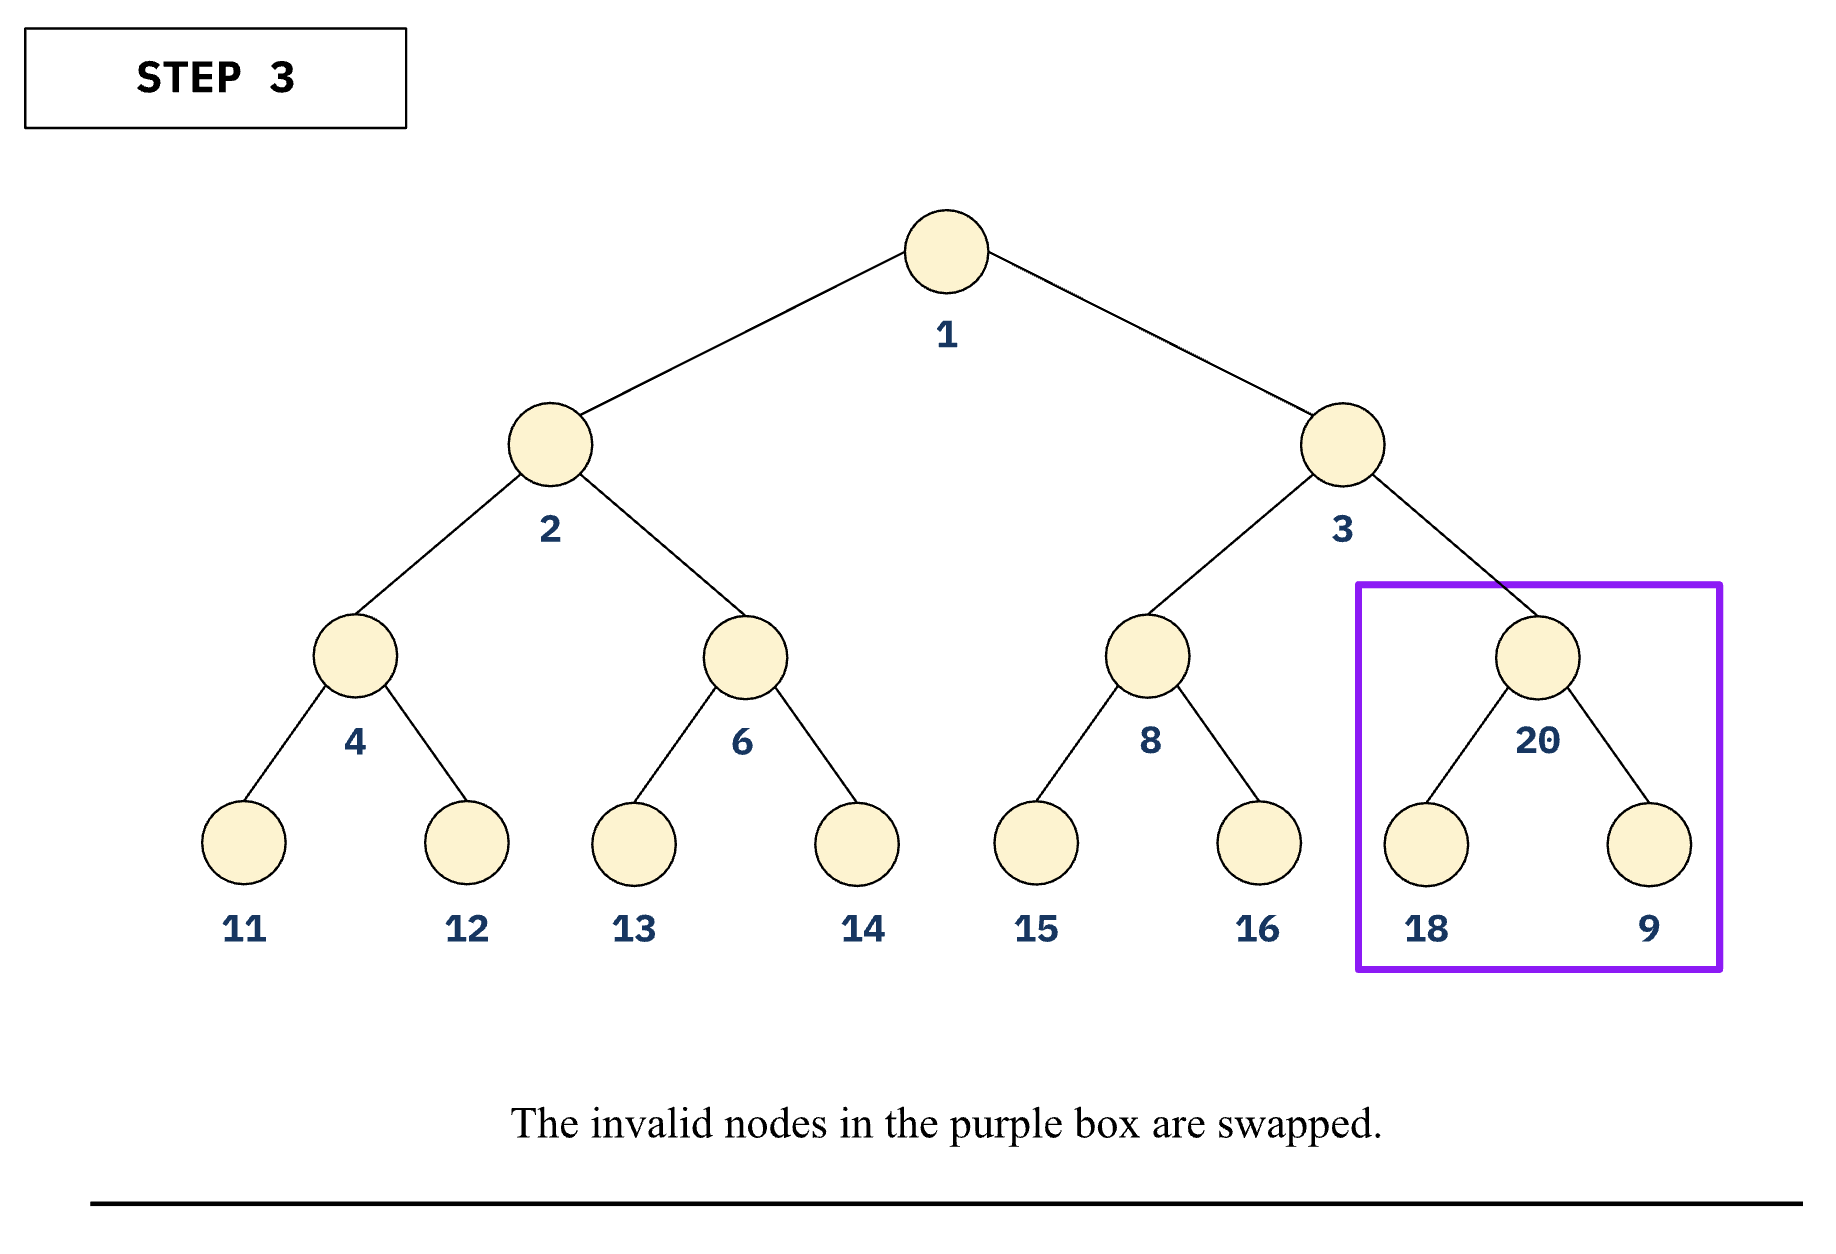
\includegraphics[width=0.72\linewidth]{Google Drawings/floyd-3.png}
    \end{subfigure}
\end{figure}
\begin{figure}[H]
    \ContinuedFloat
    \begin{subfigure}{\textwidth}
        \centering
        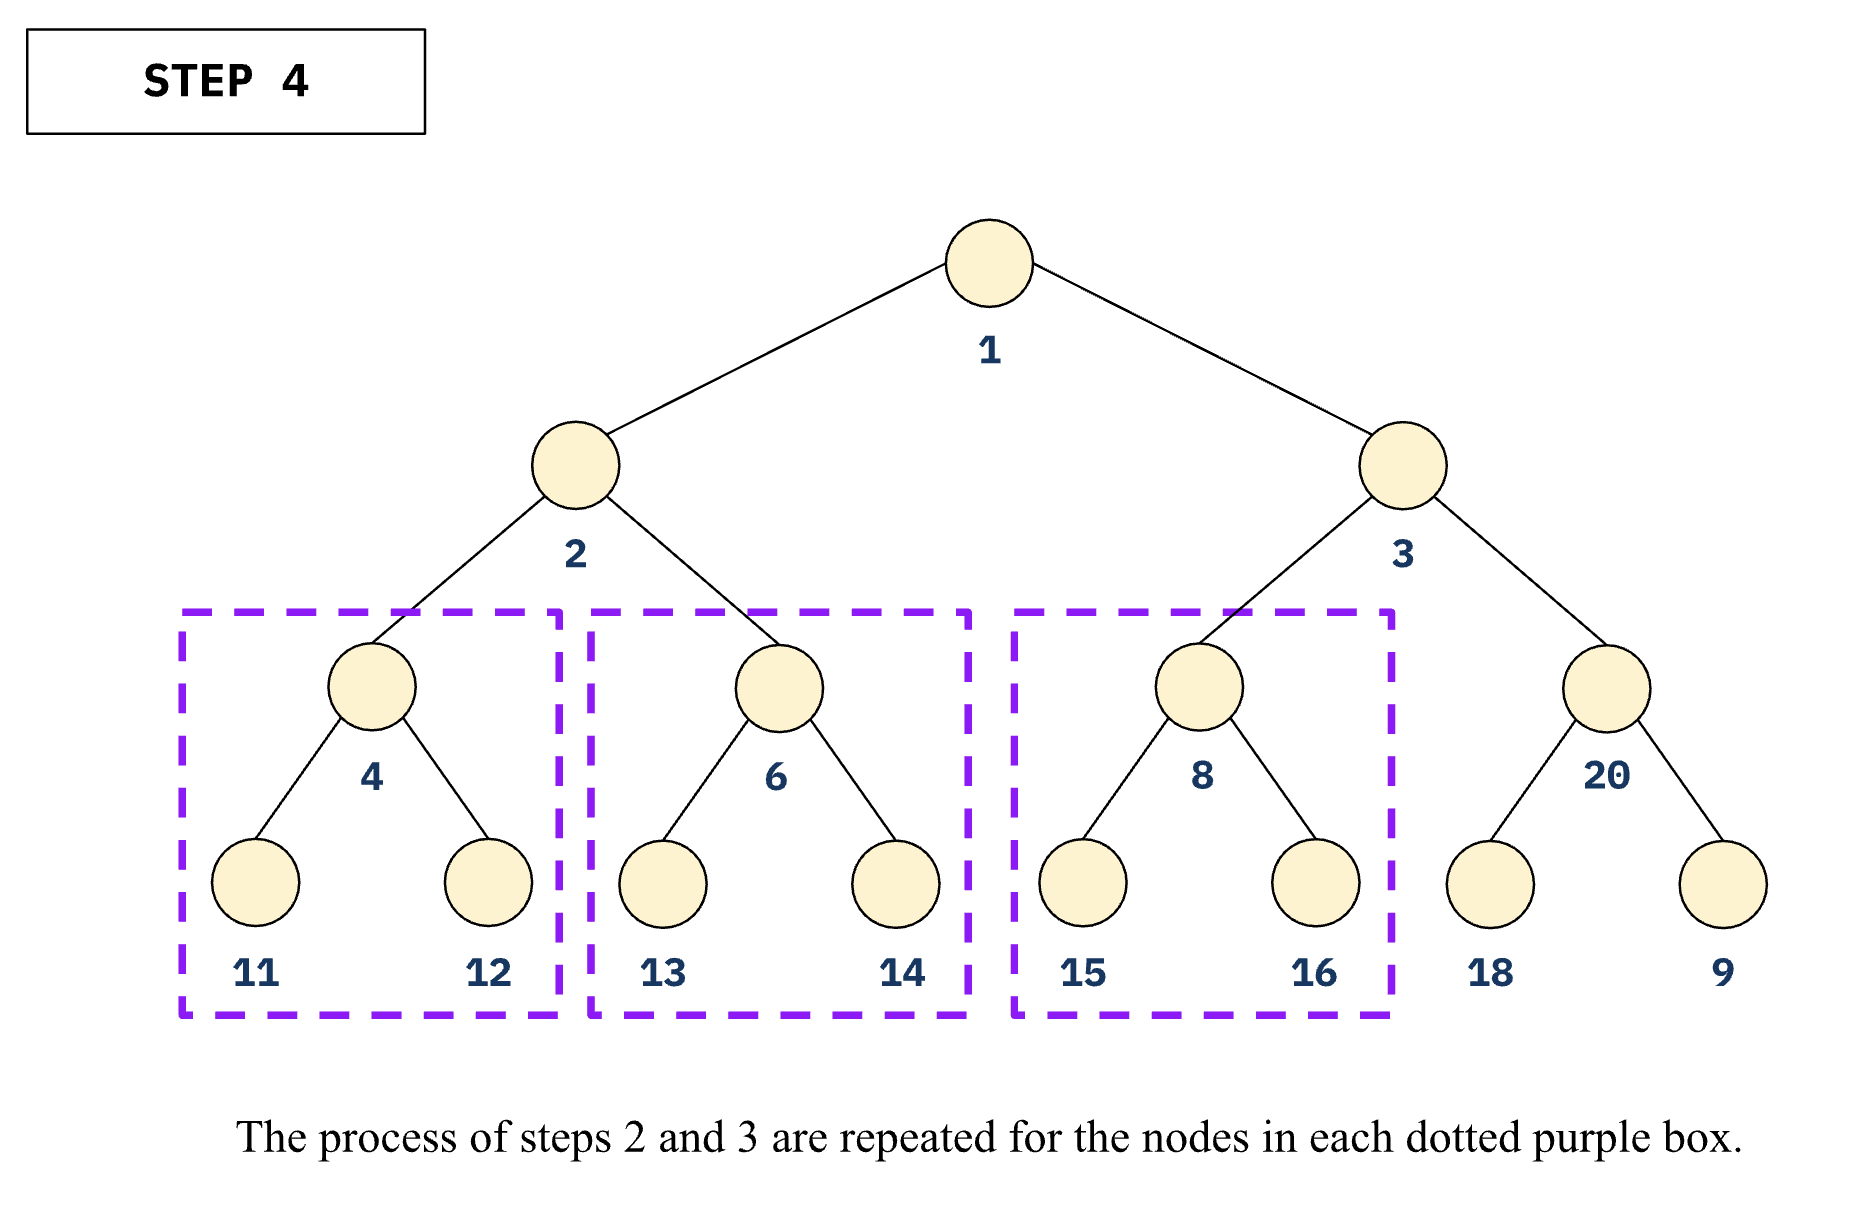
\includegraphics[width=0.72\linewidth]{Google Drawings/floyd-4.png}
    \end{subfigure}
    \begin{subfigure}{\textwidth}
        \centering
        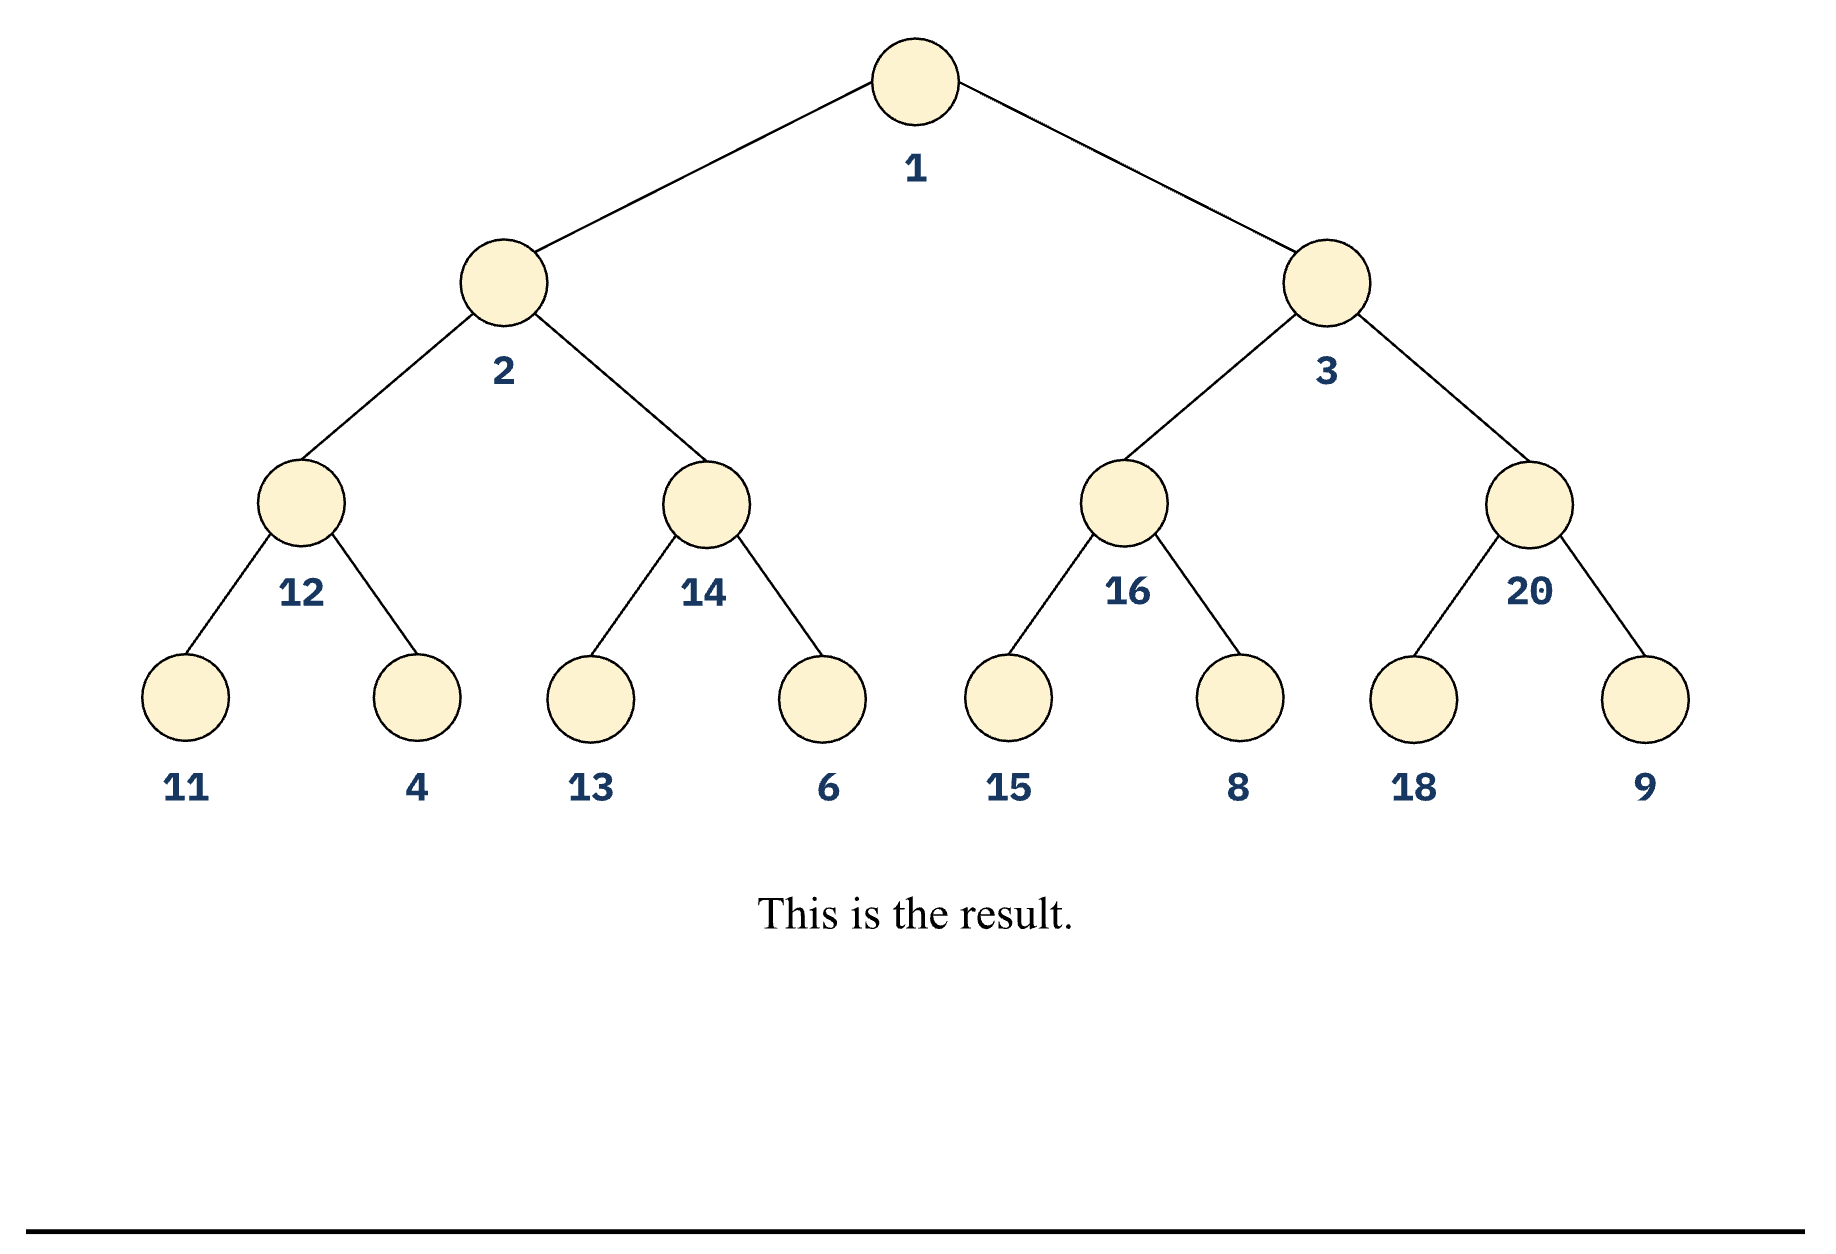
\includegraphics[width=0.72\linewidth]{Google Drawings/floyd-4a.png}
    \end{subfigure}
    \begin{subfigure}{\textwidth}
        \centering
        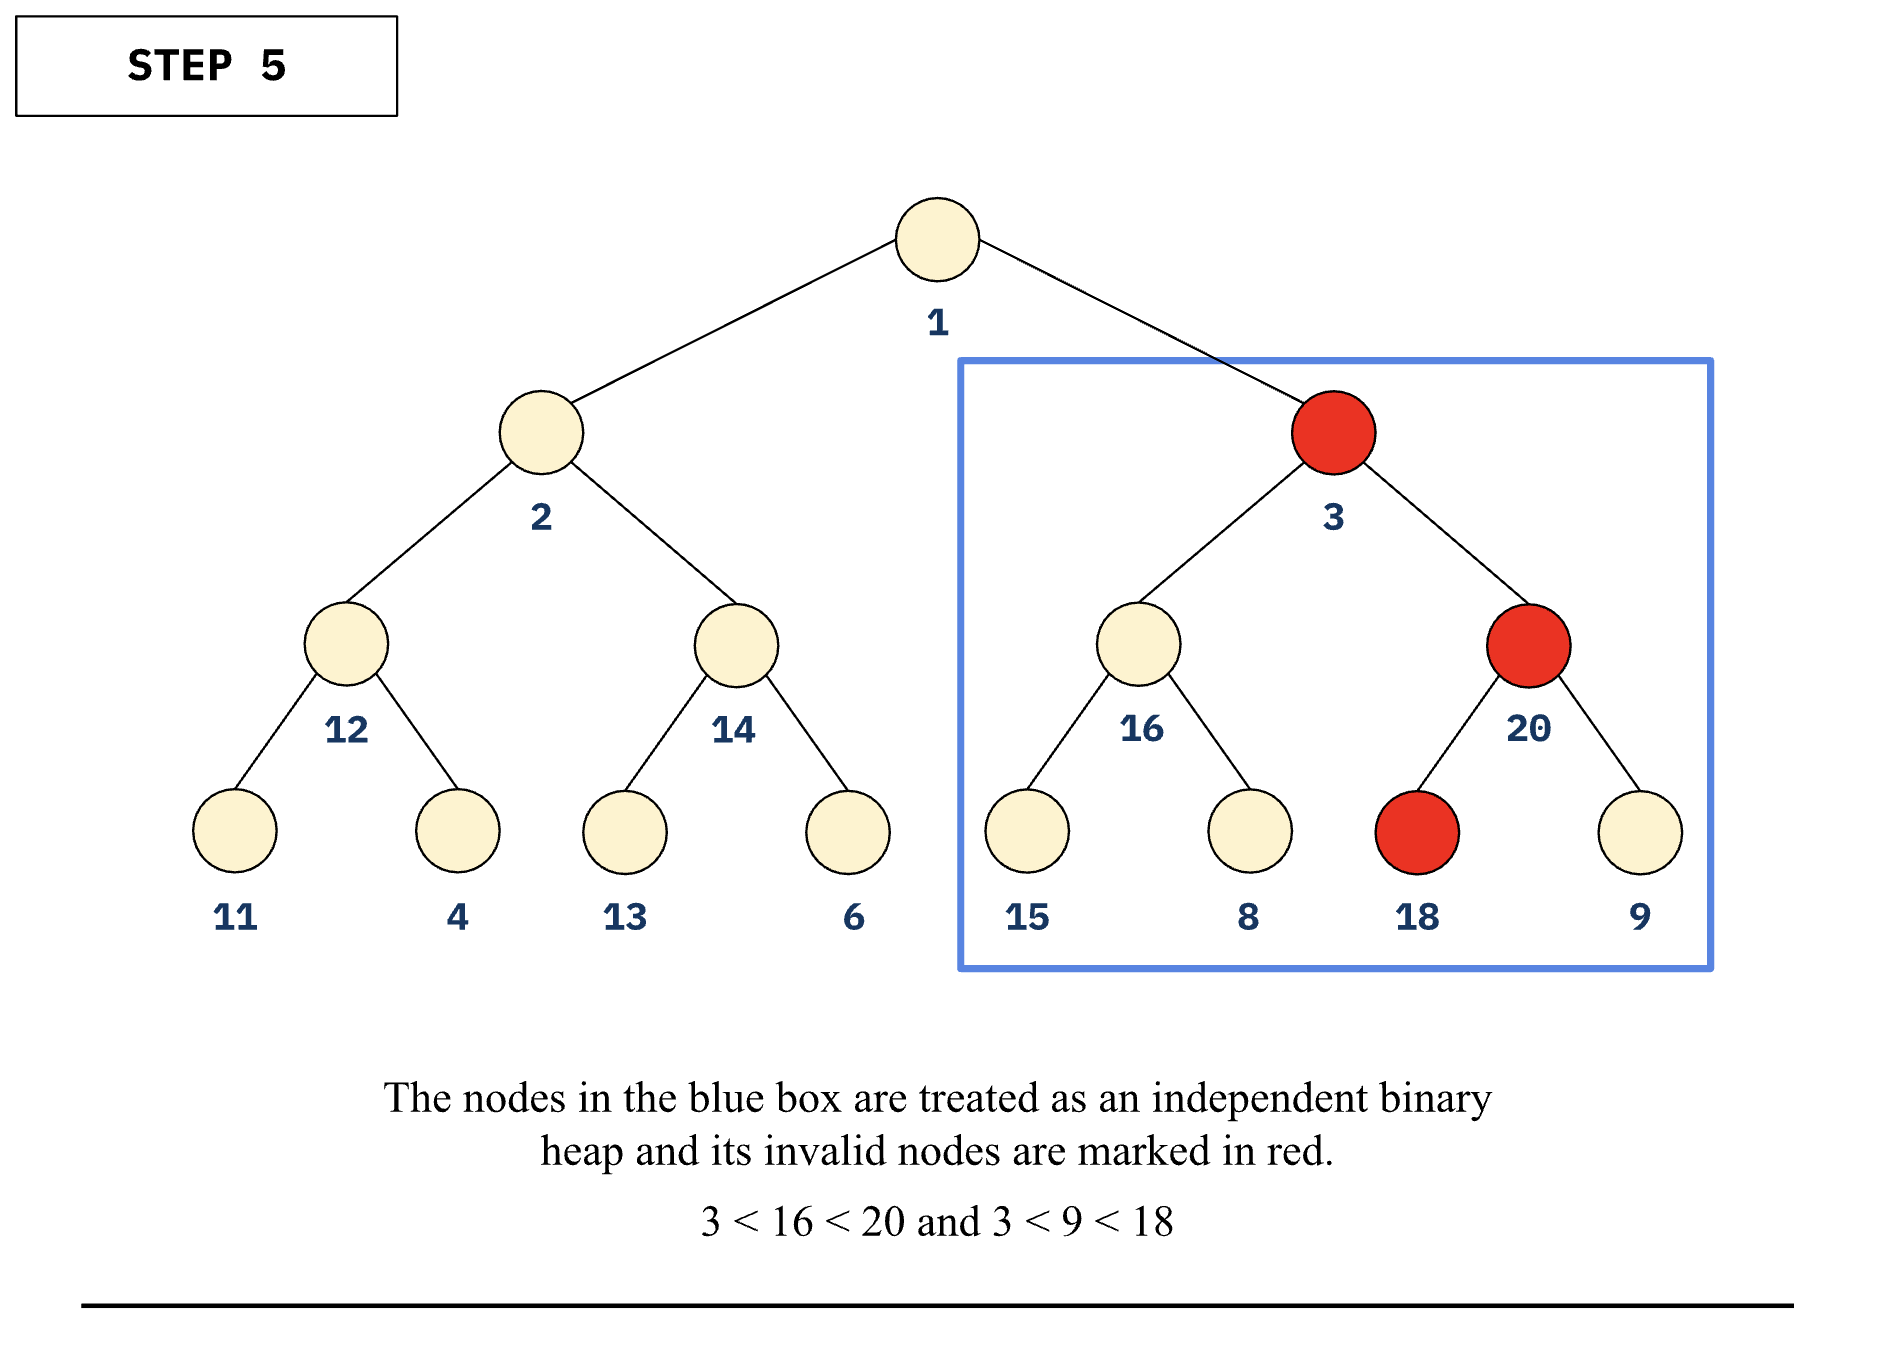
\includegraphics[width=0.72\linewidth]{Google Drawings/floyd-5.png}
    \end{subfigure}
\end{figure}
\begin{figure}[H]
    \ContinuedFloat
    \begin{subfigure}{\textwidth}
        \centering
        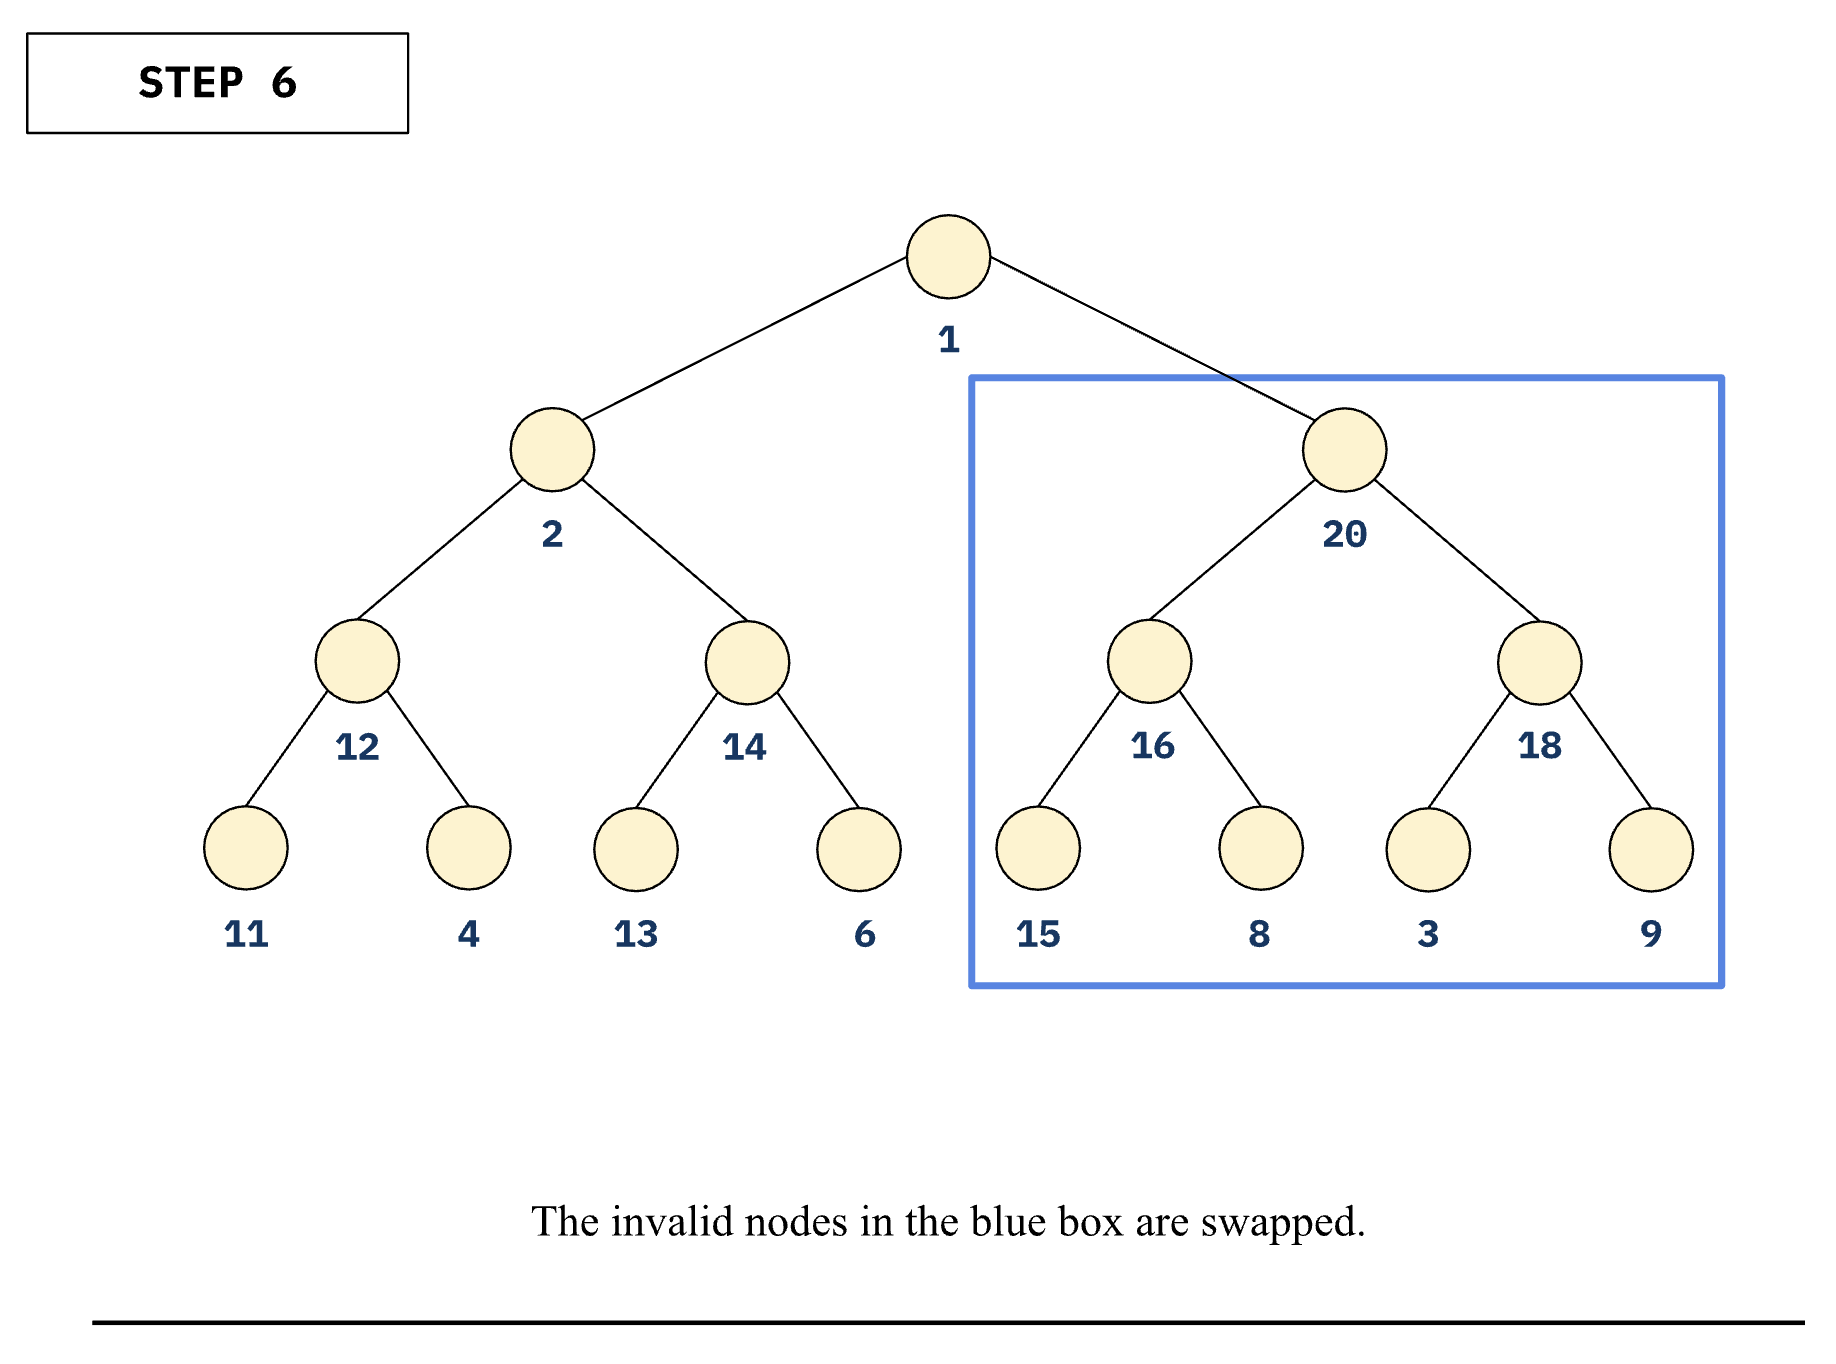
\includegraphics[width=0.72\linewidth]{Google Drawings/floyd-6.png}
    \end{subfigure}
    \begin{subfigure}{\textwidth}
        \centering
        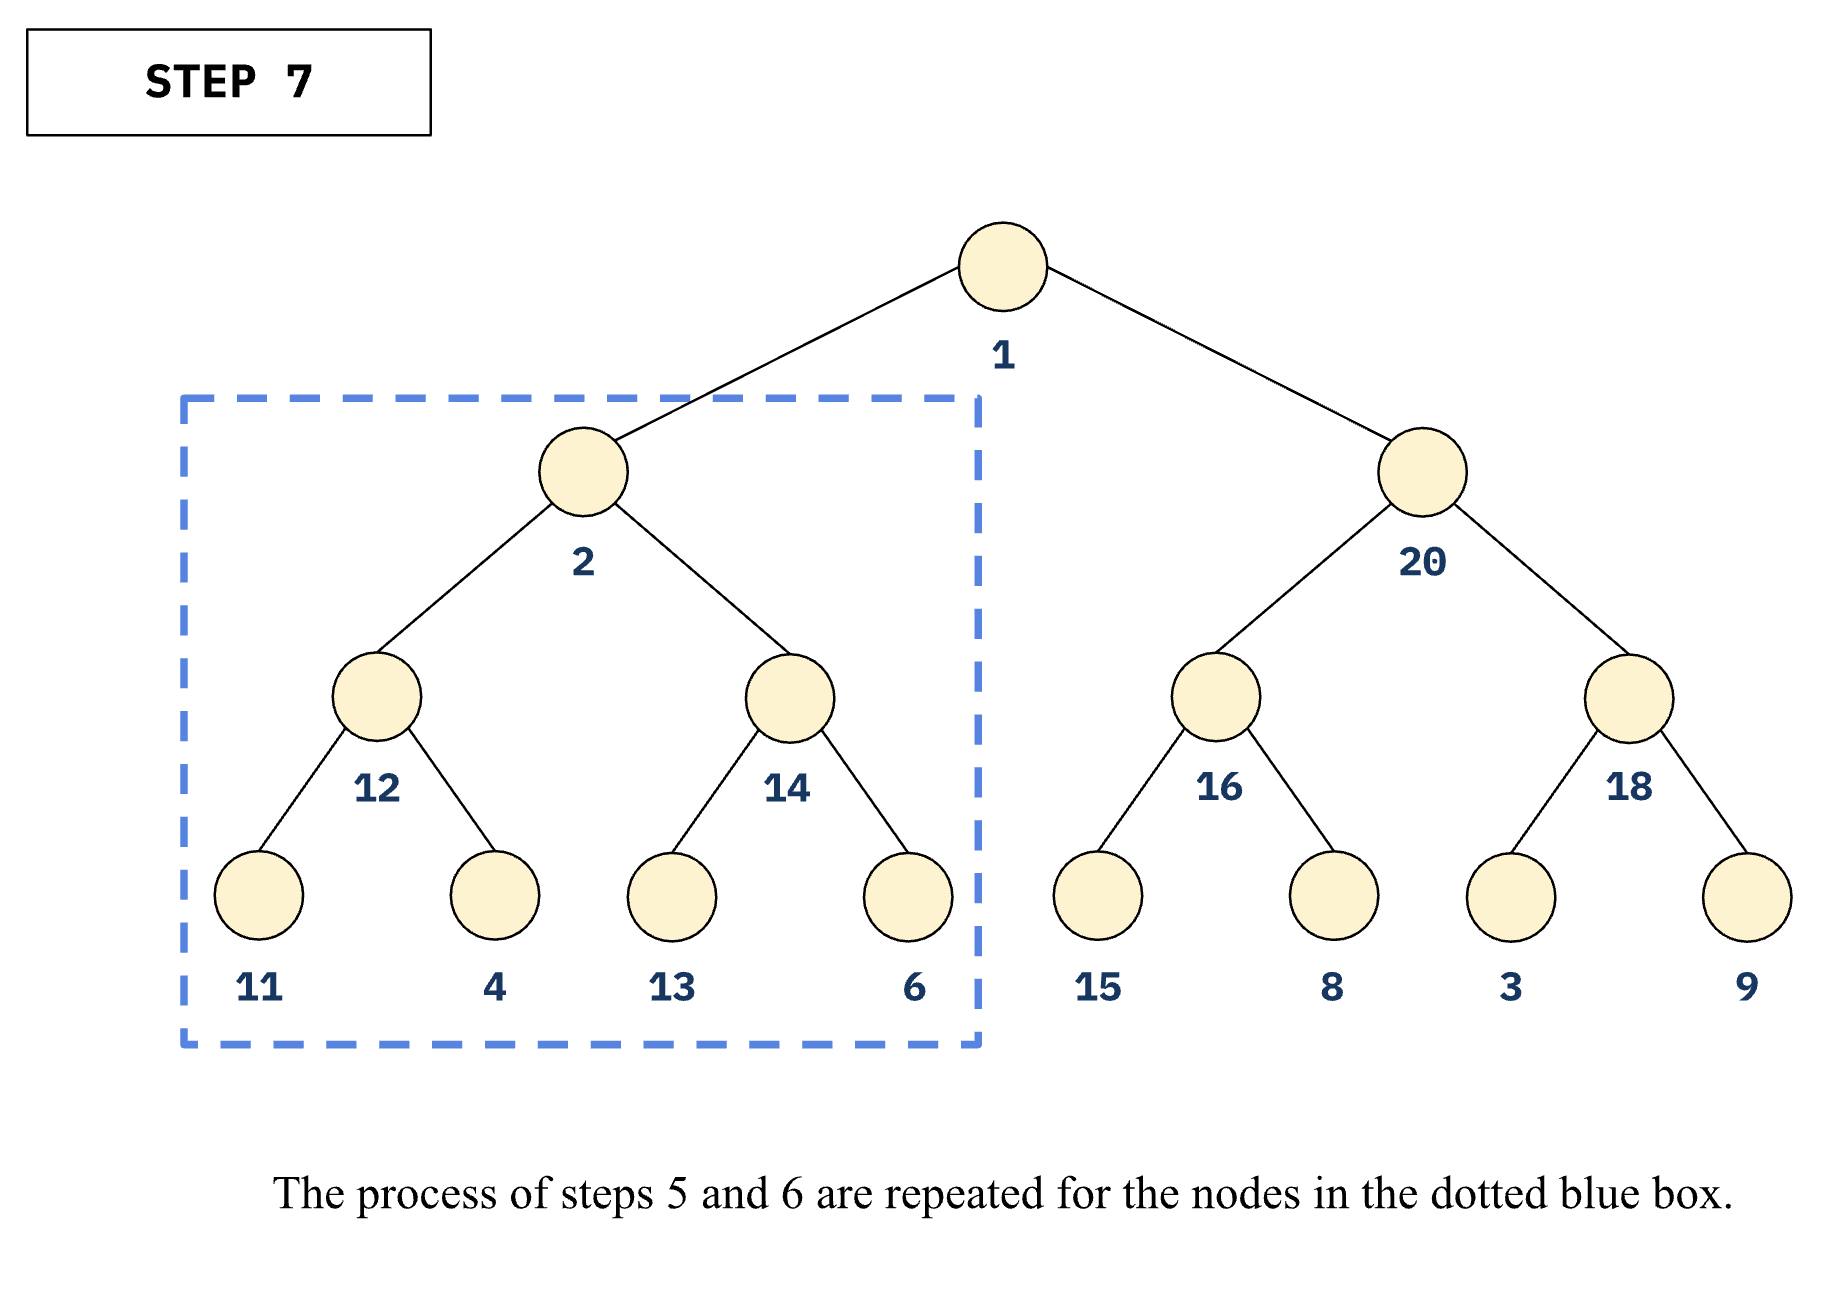
\includegraphics[width=0.72\linewidth]{Google Drawings/floyd-7.png}
    \end{subfigure}
    \begin{subfigure}{\textwidth}
        \centering
        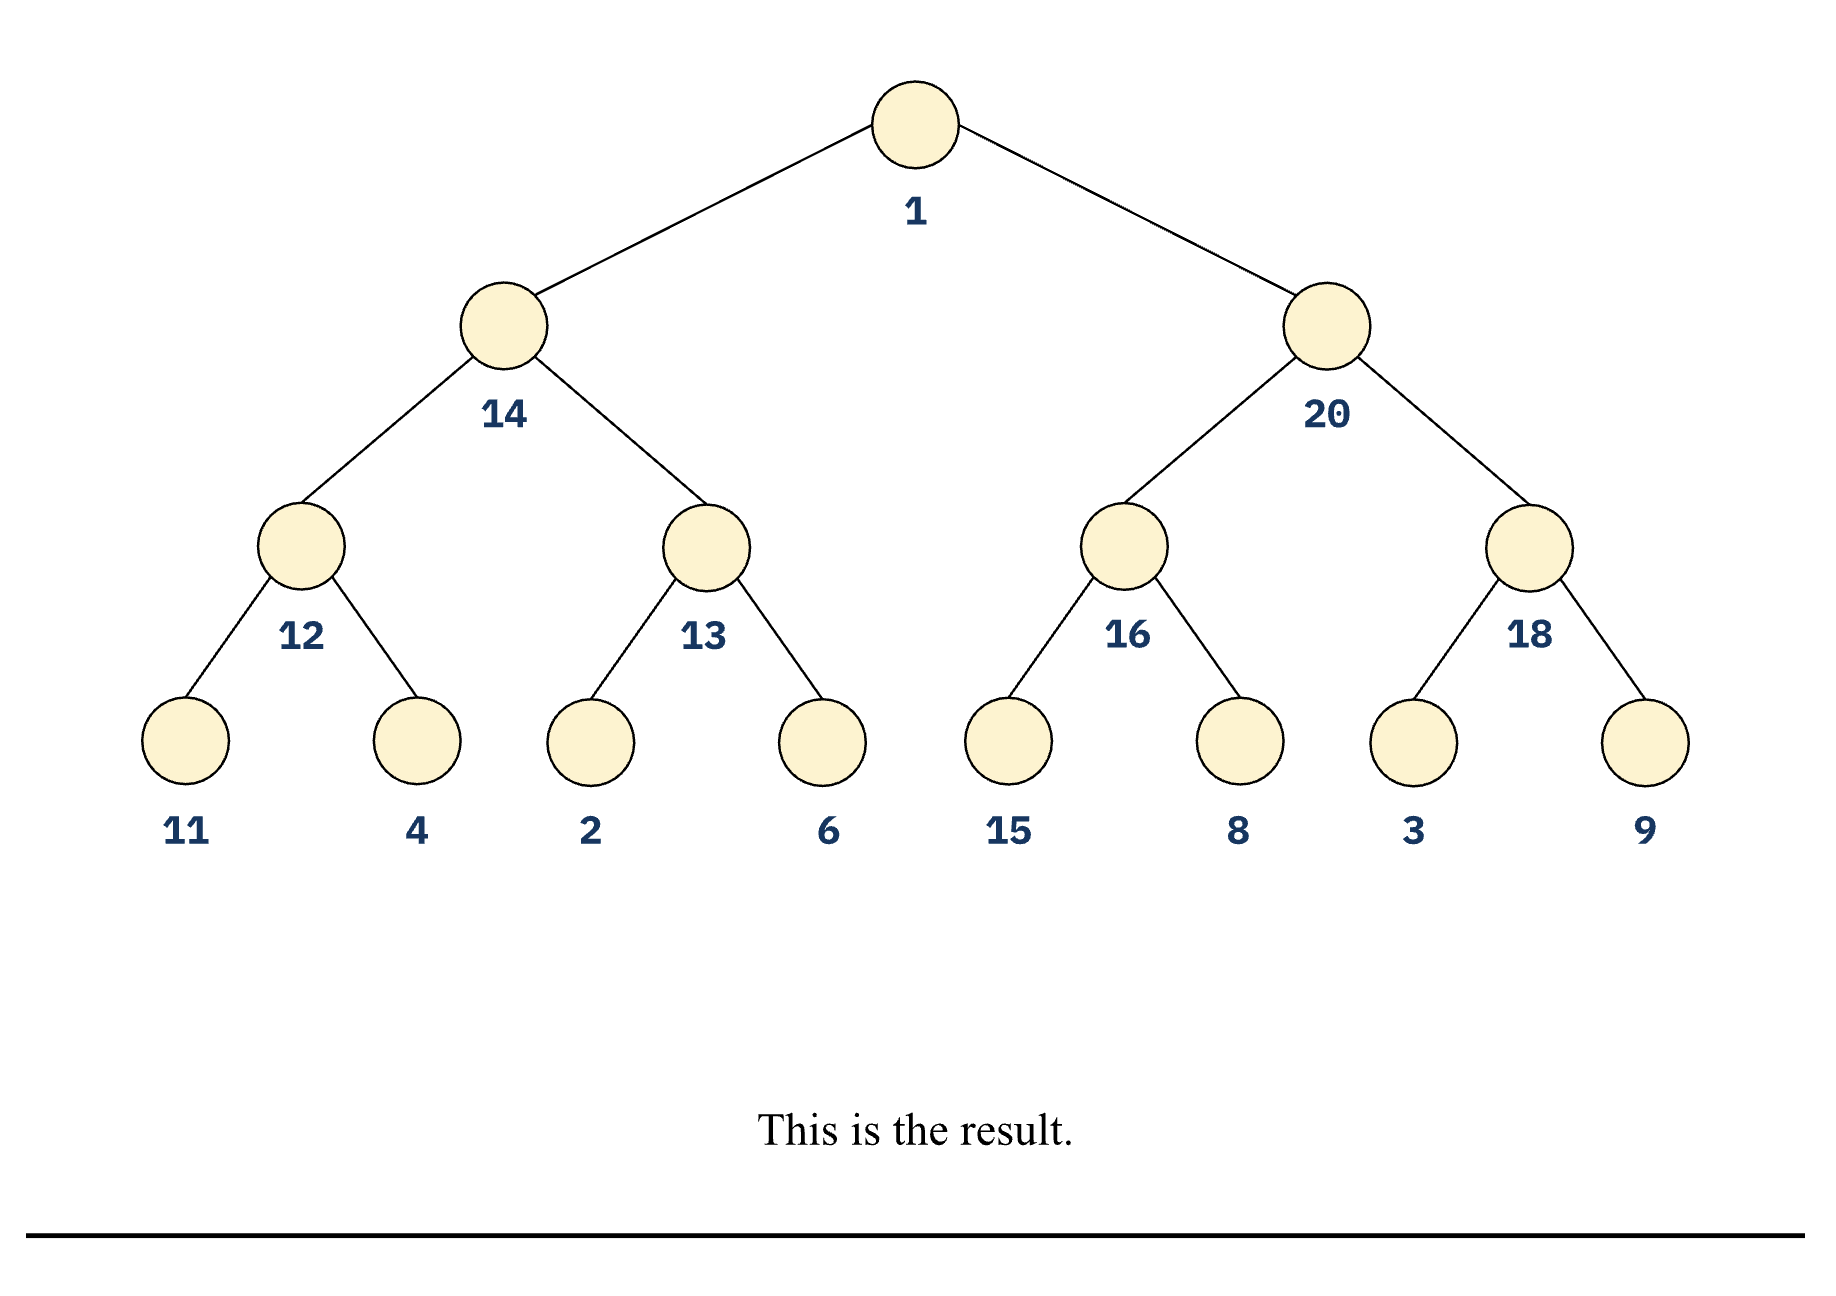
\includegraphics[width=0.72\linewidth]{Google Drawings/floyd-7a.png}
    \end{subfigure}
\end{figure}
\begin{figure}[H]
    \ContinuedFloat
    \begin{subfigure}{\textwidth}
        \centering
        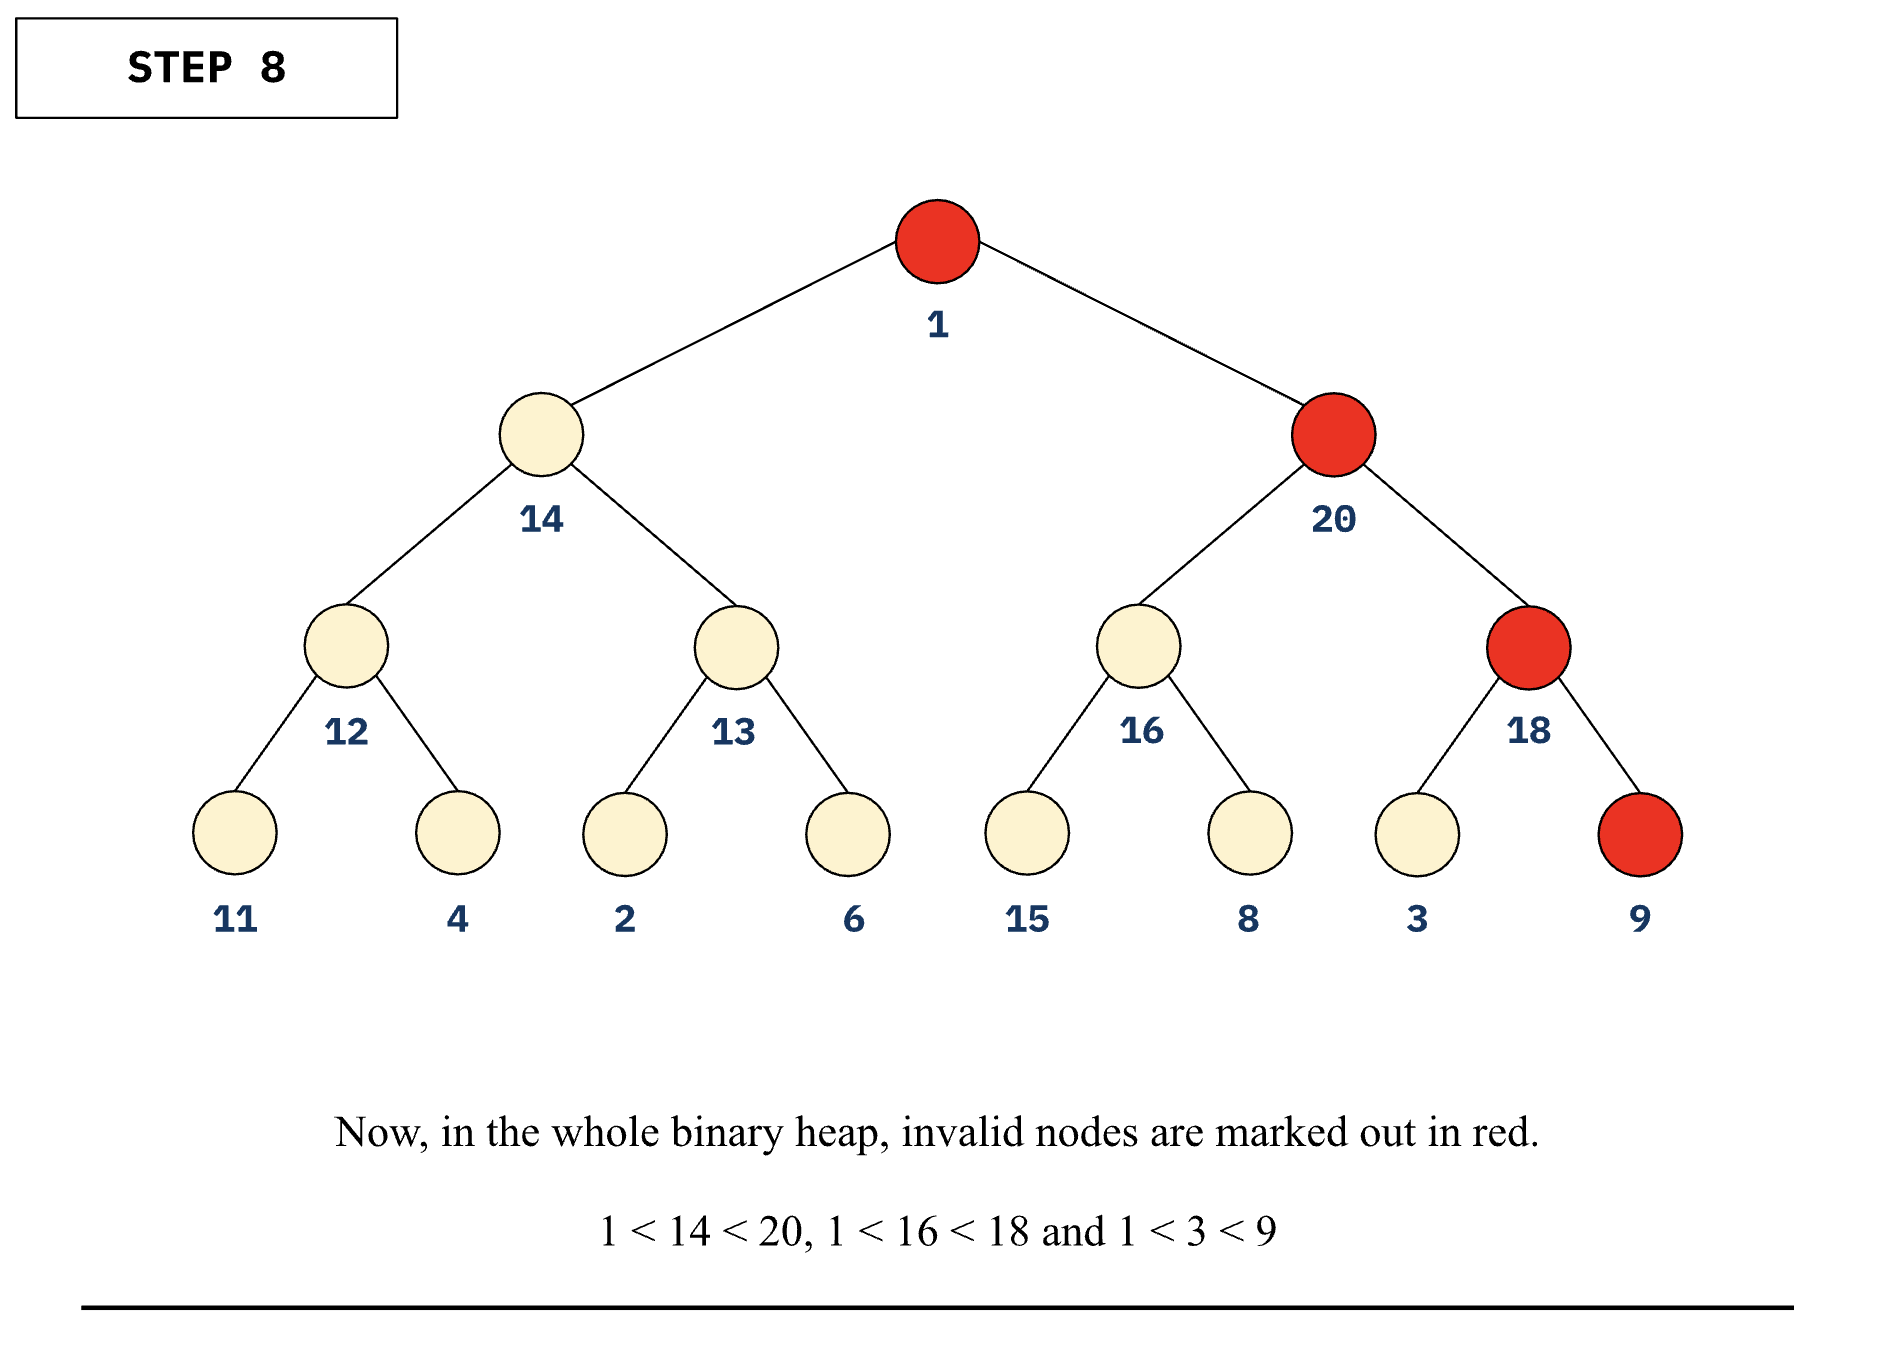
\includegraphics[width=0.72\linewidth]{Google Drawings/floyd-8.png}
    \end{subfigure}
    \begin{subfigure}{\textwidth}
        \centering
        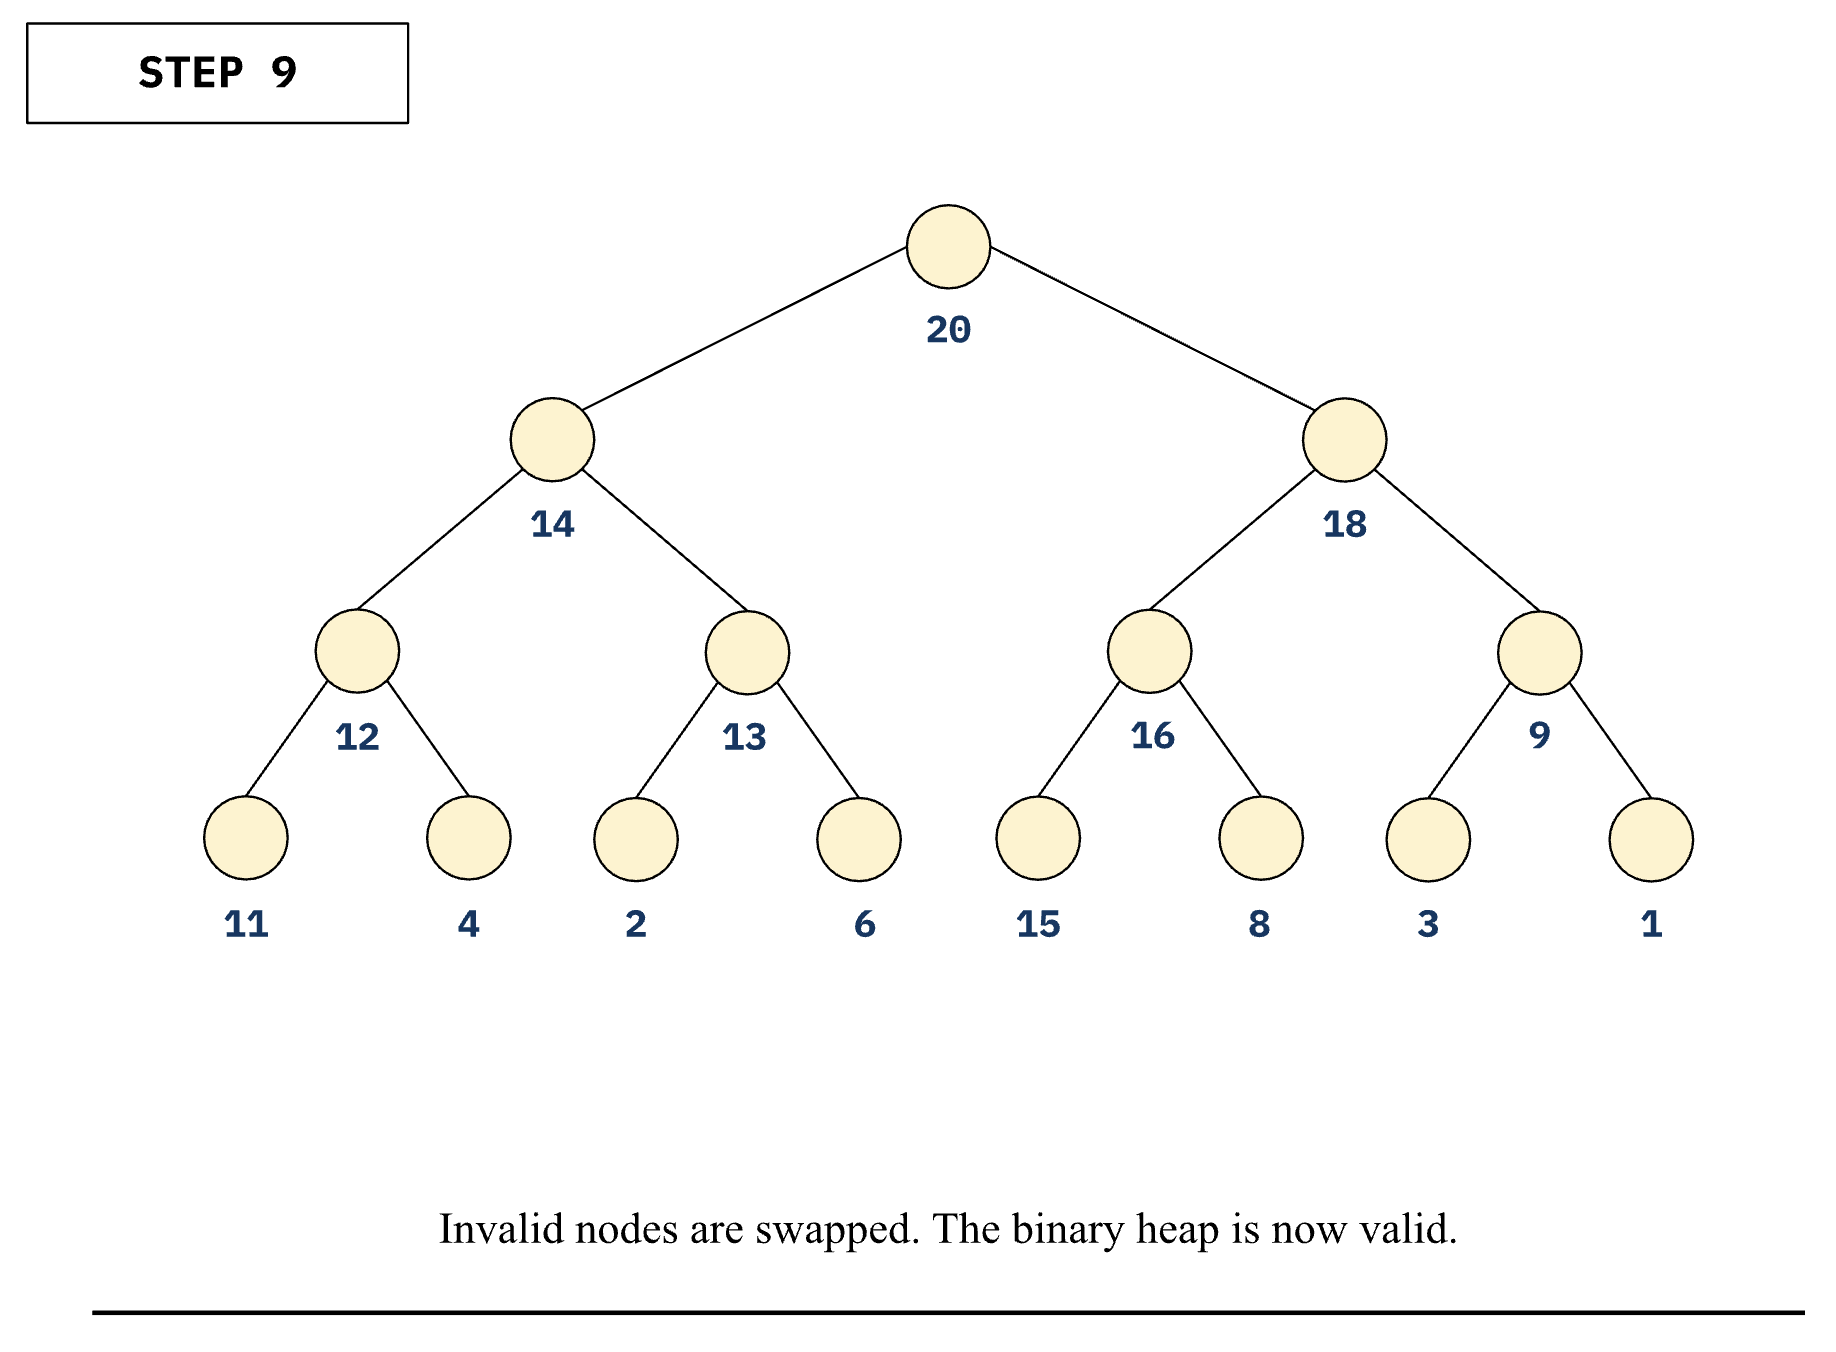
\includegraphics[width=0.72\linewidth]{Google Drawings/floyd-9.png}
    \end{subfigure}
\end{figure}

In the figure above, notice that when a parent node has a lower priority than one or both its child nodes, the child node with the higher priority swaps with the parent node. This is to ensure that the priority of the new parent node will be greater than that of both its child nodes.\newline

Floyd’s method, as demonstrated in figure \ref{fig:floyd-creation}, conceptually breaks down an invalid binary heap into smaller parts. What is not shown in figure \ref{fig:floyd-creation} is that each node at the bottom level is first treated as an independent binary heap, indicated by the red boxes shown in figure \ref{fig:floyd-breakdown}.

\begin{figure}[H]
    \centering
    \caption{Floyd's method breakdown}
    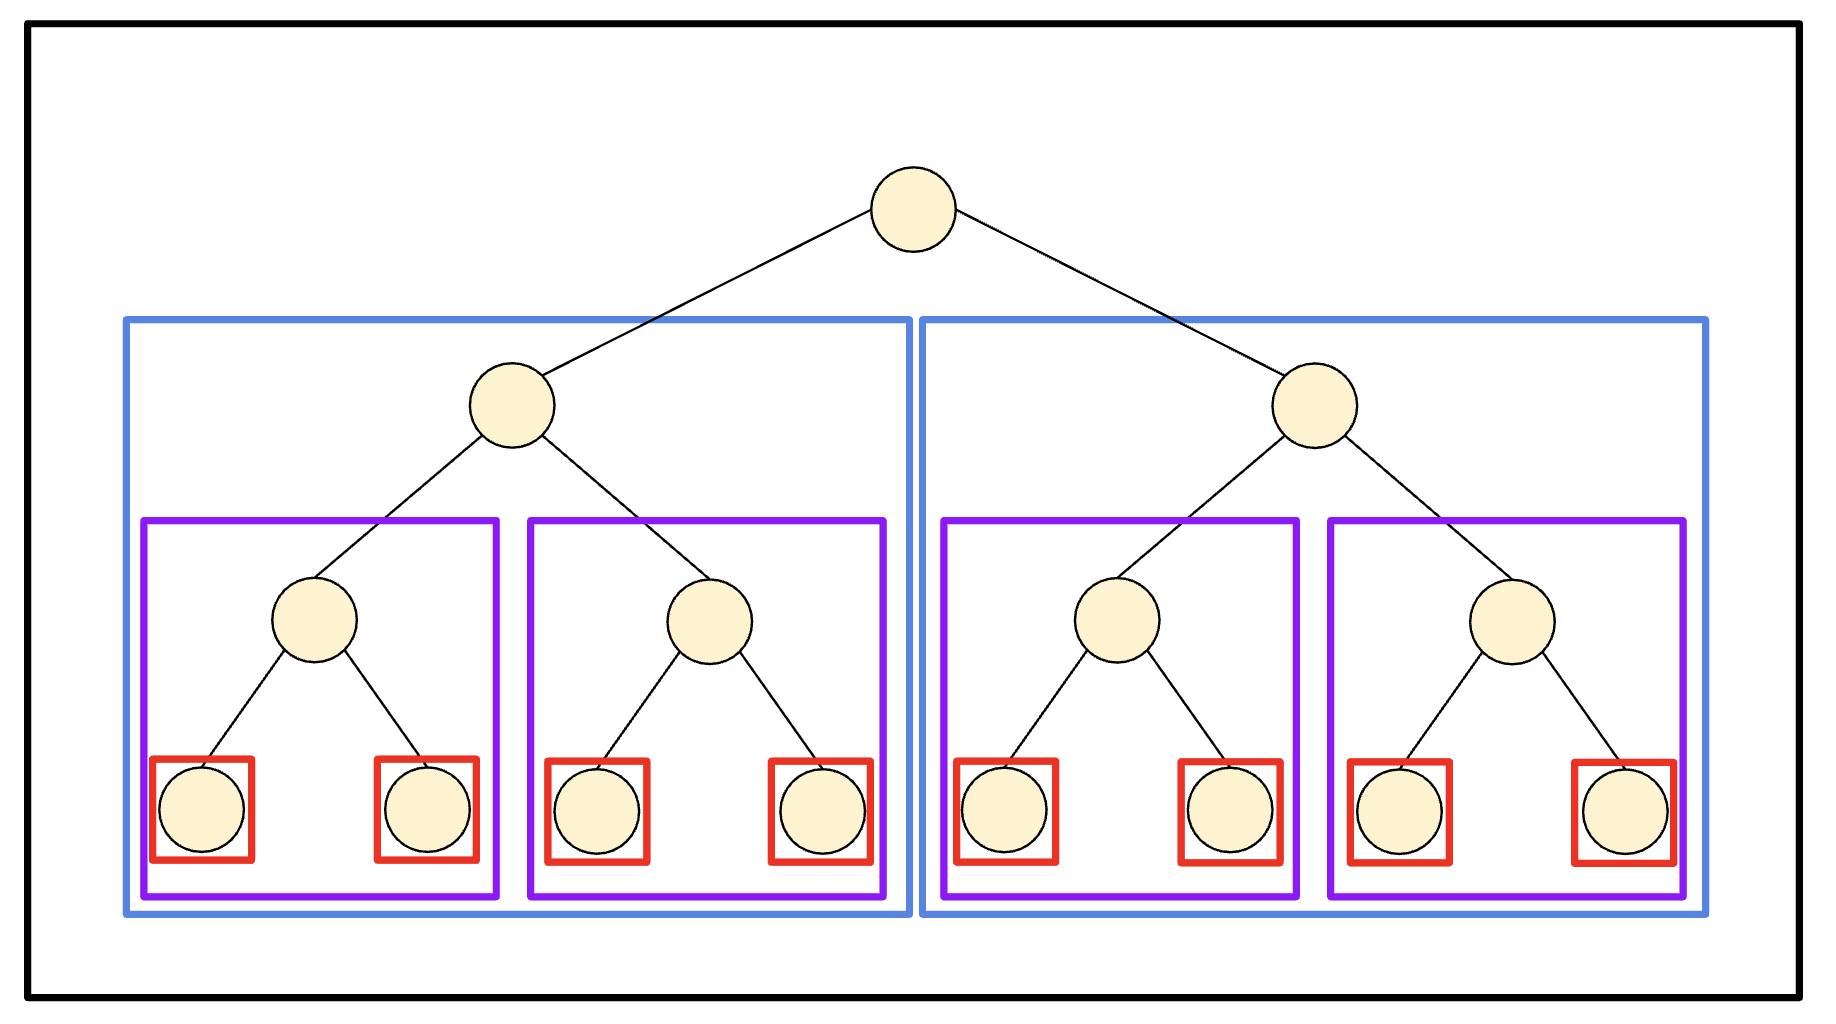
\includegraphics[width=0.75\linewidth]{Google Drawings/floyd-breakdown.png}
    \label{fig:floyd-breakdown}
\end{figure}

Since a binary heap containing one node is always sorted, no swaps occur within the red boxes. Next, the nodes in the purple boxes are rearranged, followed by the nodes in the blue boxes and finally with the entire binary heap. In each of the boxes that the original binary heap is split into, nodes are swapped so that they become a valid binary heap \parencite[13]{washu_floyd_proof}. Figures \ref{fig:floyd-creation} and \ref{fig:floyd-breakdown} both use an example of a binary heap with $N=15$, but this process applies to binary heaps of all positive integer values of $N$.\newline

To investigate why Floyd’s method is faster than Williams’s method, I will need to obtain the OOG of the OPS function of Floyd’s method so that it can be compared to that of Williams’s method.\newline

\subsection{Obtaining the OPS function}
We shall assume a worst case scenario where all elements that are being added to the binary heap would have a higher priority than the previous element, with the root node having the lowest priority before any swapping has occurred. In order to find the OOG of the OPS function of Floyd’s method, I would need to obtain the relationship between $N$ and the total number of operations, which is the number of swaps, needed for the creation of a binary heap.\newline

Figure \ref{fig:swapping1-floyd} shows the first 2 groups of nodes that are rearranged with a binary heap of $N$ elements, with all parent nodes having a lower priority than both their child nodes. 

\begin{figure}[H]
    \centering
    \caption{Swapping of nodes at level $H-1$}
    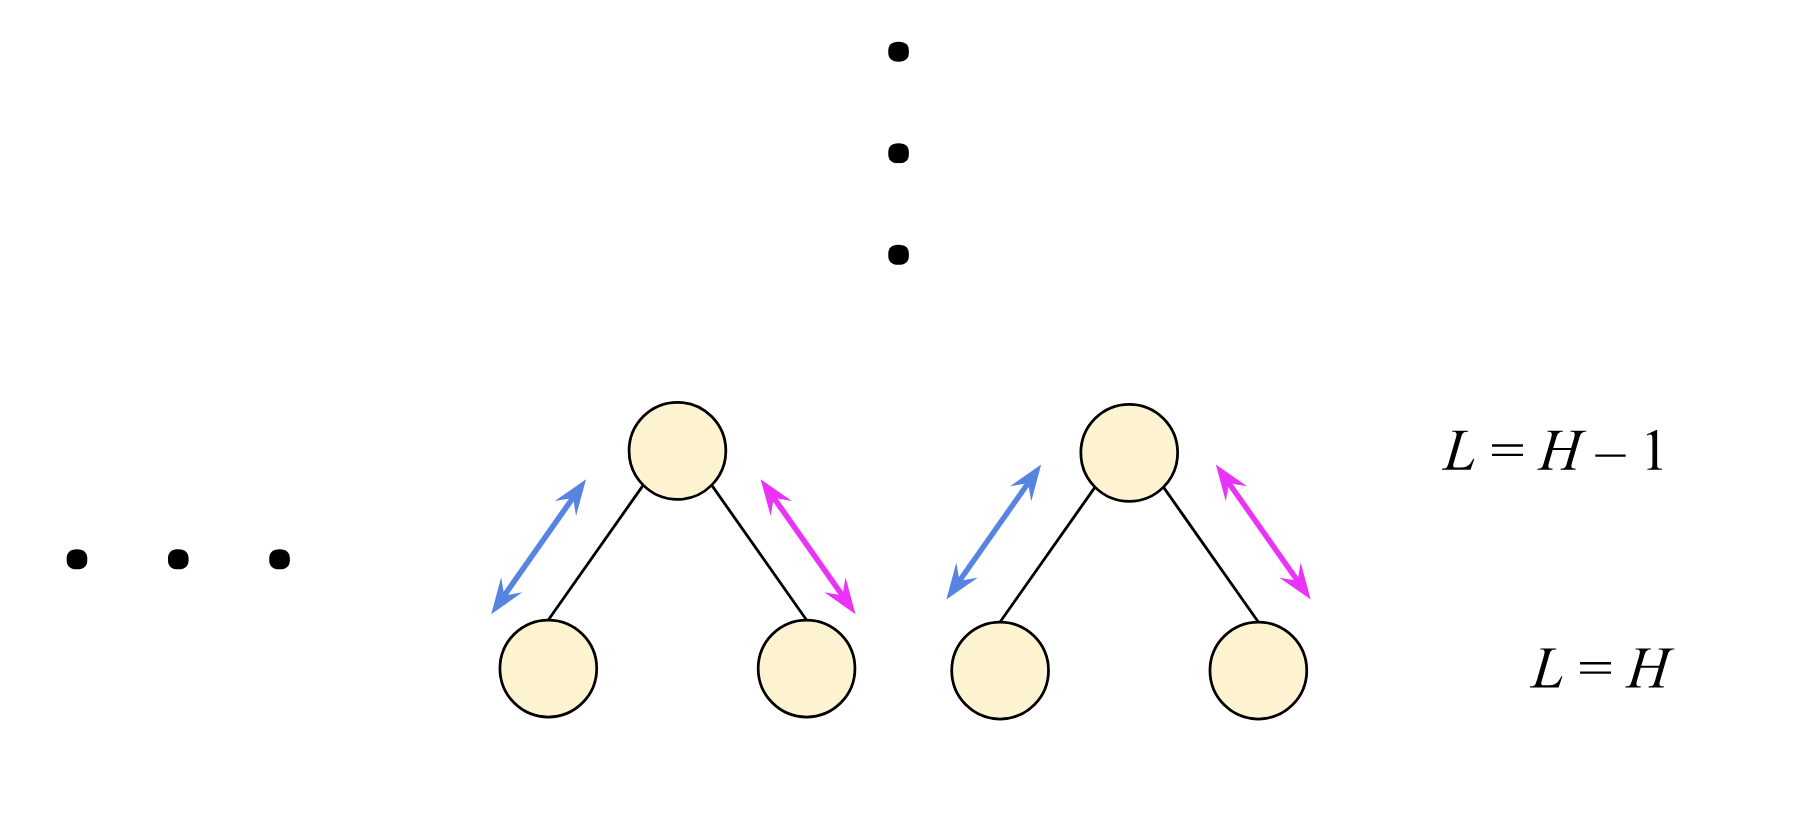
\includegraphics[width=0.75\linewidth]{Google Drawings/swapping-at-level-h-minus-1-v2.png}
    \label{fig:swapping1-floyd}
\end{figure}

The parent nodes at $L=H-1$ are either swapped with its left child node or its right child node, depending on which of the two child nodes has the highest priority. This means that there is a maximum of 1 operation done for each node at $L=H-1$.\newline

Once all the nodes at $L=H-1$ are swapped, Floyd’s method would then swap invalid nodes at $L=H-2$, depicted in Figure \ref{fig:swapping2-floyd}.

\begin{figure}[H]
    \centering
    \caption{Swapping of nodes at level $H-2$}
    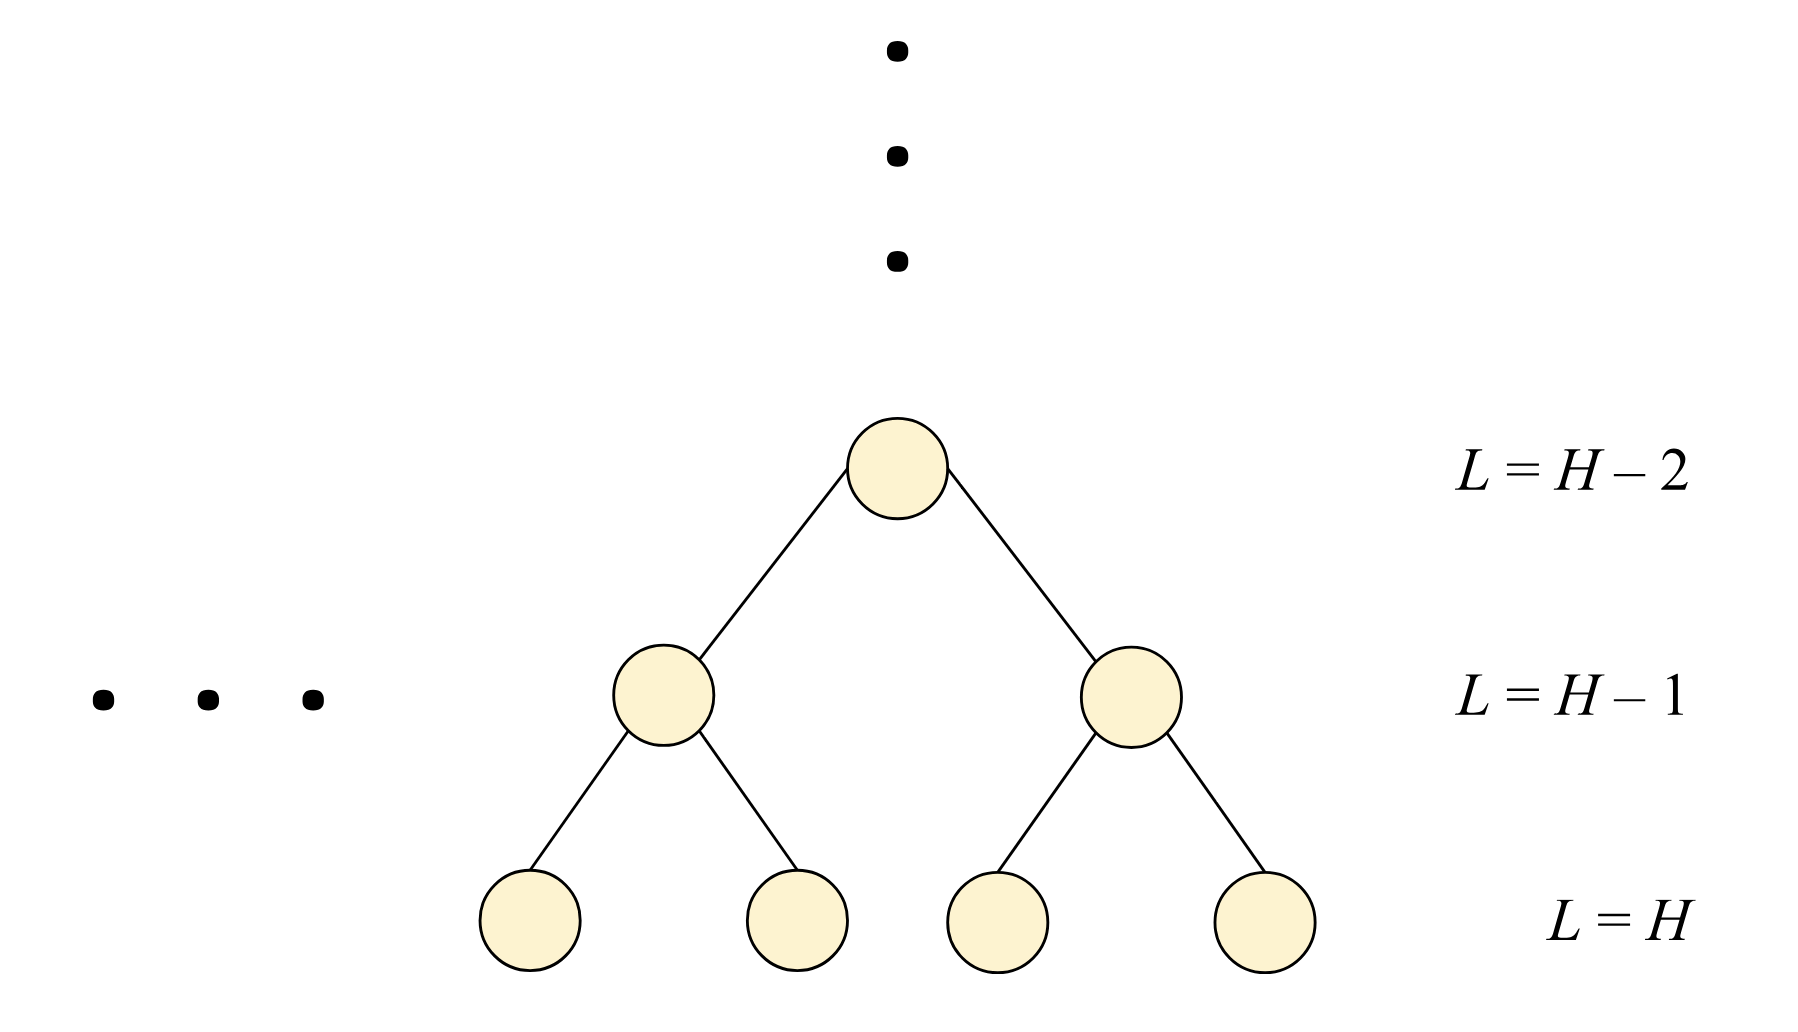
\includegraphics[width=0.75\linewidth]{Google Drawings/swapping-at-level-h-minus-2-v2.png}
    \label{fig:swapping2-floyd}
\end{figure}

In a worst case scenario, the maximum number of swaps for nodes on a certain level is equal to how many levels they are from the bottom of the binary heap as nodes can only be swapped with their own child nodes. Since nodes at $L=H-2$ are $2$ levels from level $H$, we can say that there is a maximum of $2$ operations done for every node at $L=H-2$. By representing the maximum number of operations per node at level $L$ as $M$, I am able to find $M$ in terms $L$ and $H$:
\vspace{-1em}
\begin{align}
    L&=H-M\nonumber\\
    L+M&=H\nonumber\\
    M&=H-L\label{eqn:M_ito_H_L}
\end{align}

Now, recalling the definition and use of $L$ from section \ref{pq_as_bin}, the maximum number of operations of all nodes at level $L$ is $2^L\times M$. By substituting $M$ as in \eqref{eqn:M_ito_H_L},\vspace{-1em}

\begin{equation*}
    \text{Max no. of operations of all nodes at level $L$ } = 2^L\times (H-L)
\end{equation*}

Hence, I can define function $F(H)$ as the total number of operations required by Floyd's method for a binary heap of height $H$, expressed as:

\[F(H)=\sum^H_{i=0}(2^i\times(H-i))\]

Recalling \eqref{eqn:N_ito_H}, I can rewrite $F(H)$ in terms of $N$ where $G(N)$ is the OPS function of Floyd's method and $G(N)\equiv F(H)$:

\[G(N)=\sum^{log_2(N+1)-1}_{i=0}(2^i\times(\log_2(N+1)-1-i))\]

By plotting the first few points of $G(N)$ in figure \ref{fig:N-G(N)-values-floyd}, we can see that the OOG of $G(N)$ is much lower than $N\log_2(N)$. In fact, it appears to have a linear OOG, with an $R^2$ value of $0.9994$ when a linear regression line of $y=0.958661N-2.54134$ is applied to the points. 

\begin{figure}[H]
    \centering
    \caption{Plotting values of $N\log_2(N)$ and $G(N)$}
    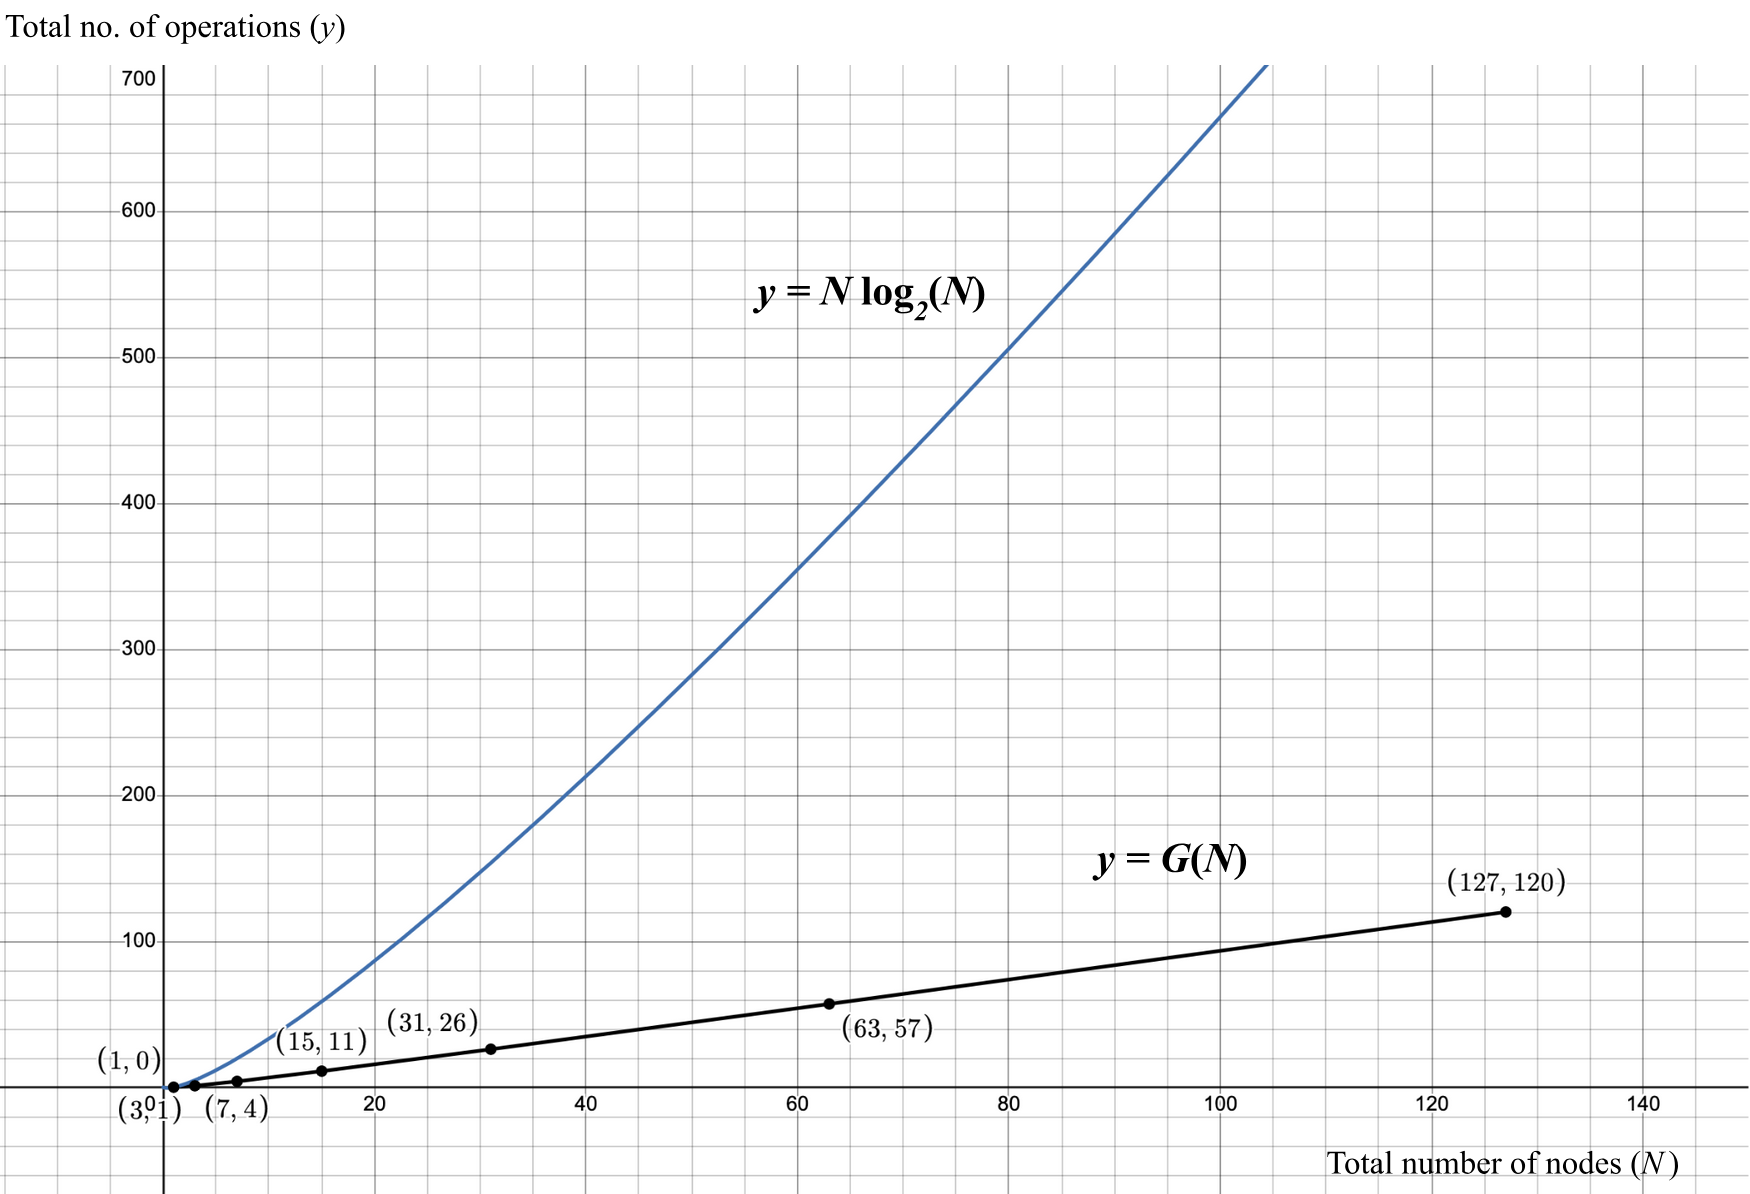
\includegraphics[width=0.75\linewidth]{Google Drawings/graph-N-and-Gn.png}
    \label{fig:N-G(N)-values-floyd}
\end{figure}

Unfortunately, concluding that $G(N)$ has a linear OOG would not be a strong claim as large values of $N$ are not found on the empirical evidence and a regression model should not be used for extrapolation; the OOG of $G(N)$ for large values of $N$ remains unknown to me.\newline

However, I realised that we could utilise geometry to analyse $F(H)=\sum^H_{i=0}(2^i\times (H-i))$ further, demonstrated in the next section.

\subsection{Use of geometry to transform the problem}
As defined previously, $F(H)$ is the summation of the maximum number of operations of all nodes at level $L$. In figure \ref{fig:geo-1-floyd}, each term in the series of $F(H)$ is drawn as a rectangle where each rectangle's area corresponds to $2^L\times (H-L)$ at different values of $L$, indicated by the purple text.

\begin{figure}[H]
    \centering
    \caption{Expressing terms in $F(H)$ using 2D geometry}
    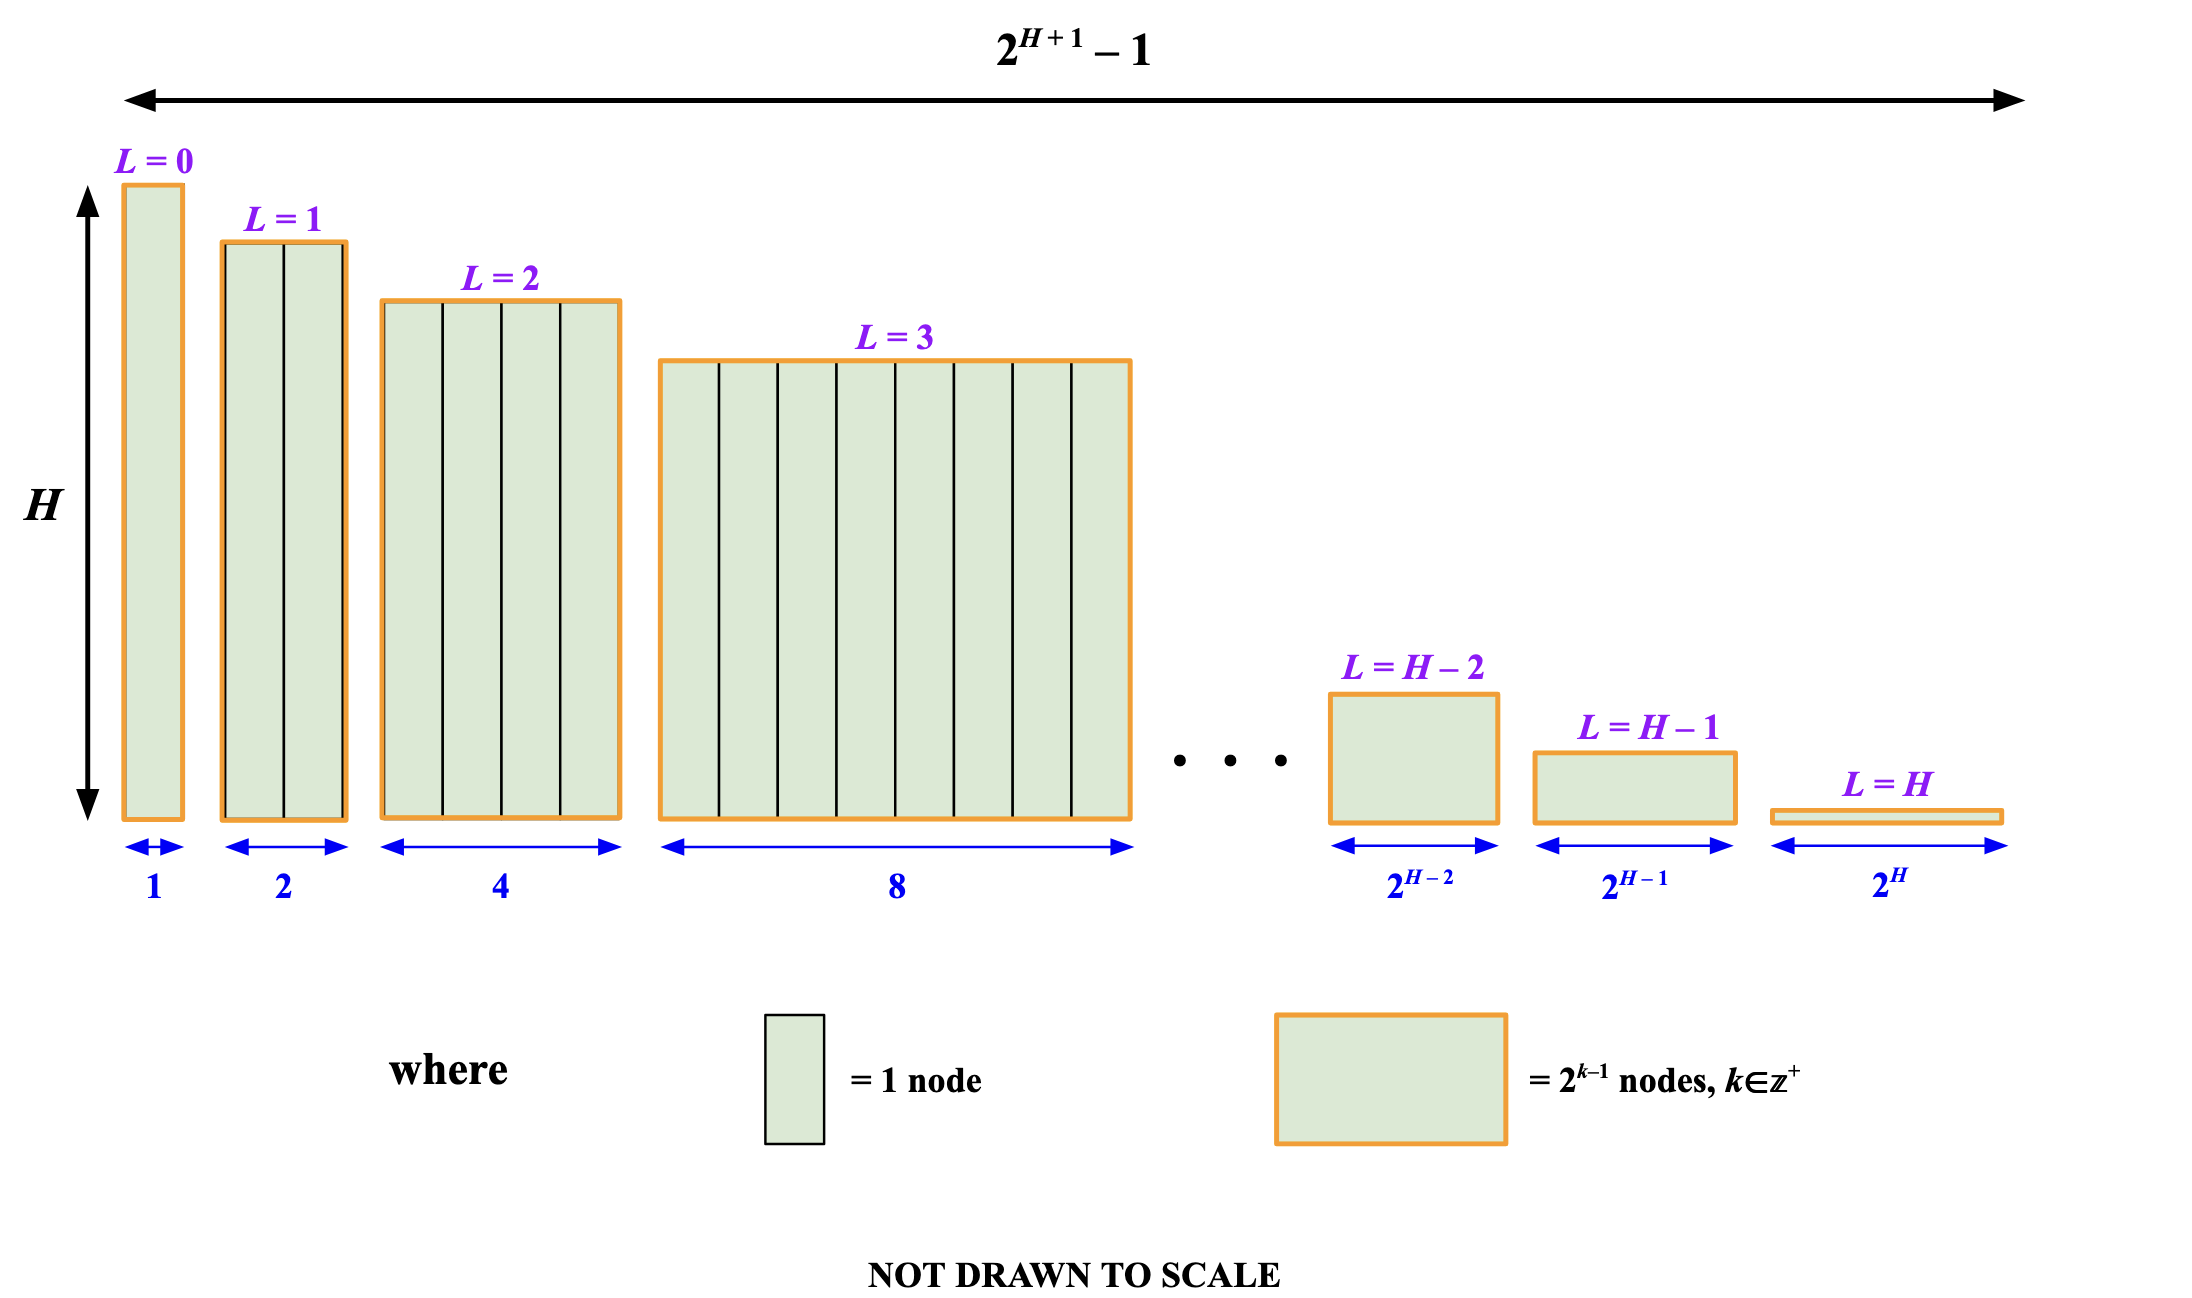
\includegraphics[width=0.9\linewidth]{Google Drawings/floyd-geometric-1-v2.png}
    \label{fig:geo-1-floyd}
\end{figure}

The width of each rectangle is represented by the number of nodes at the current level, and their respective heights represented by the maximum number of swaps for each node in that level; the number of levels from the bottom of the binary heap. By laying the rectangles side by side on the horizontal axis, we can see that the sum of their widths is the total number of nodes, $N$, which can also be expressed as $2^{H+1}-1$. $F(H)$ is therefore the total area of $H$ rectangles, one rectangle for each term in the series. Note that the last term is technically not a rectangle as it would have a height of $0$. My main goal would be to find the area of all nodes in figure \ref{fig:geo-1-floyd} such that $F(H)$ can be expressed in a way that is easier to simplify compared to $\sum^H_{i=0}(2^i\times (H-i))$.

\begin{figure}[H]
    \centering
    \caption{Splitting terms in geometric representation of $F(H)$}
    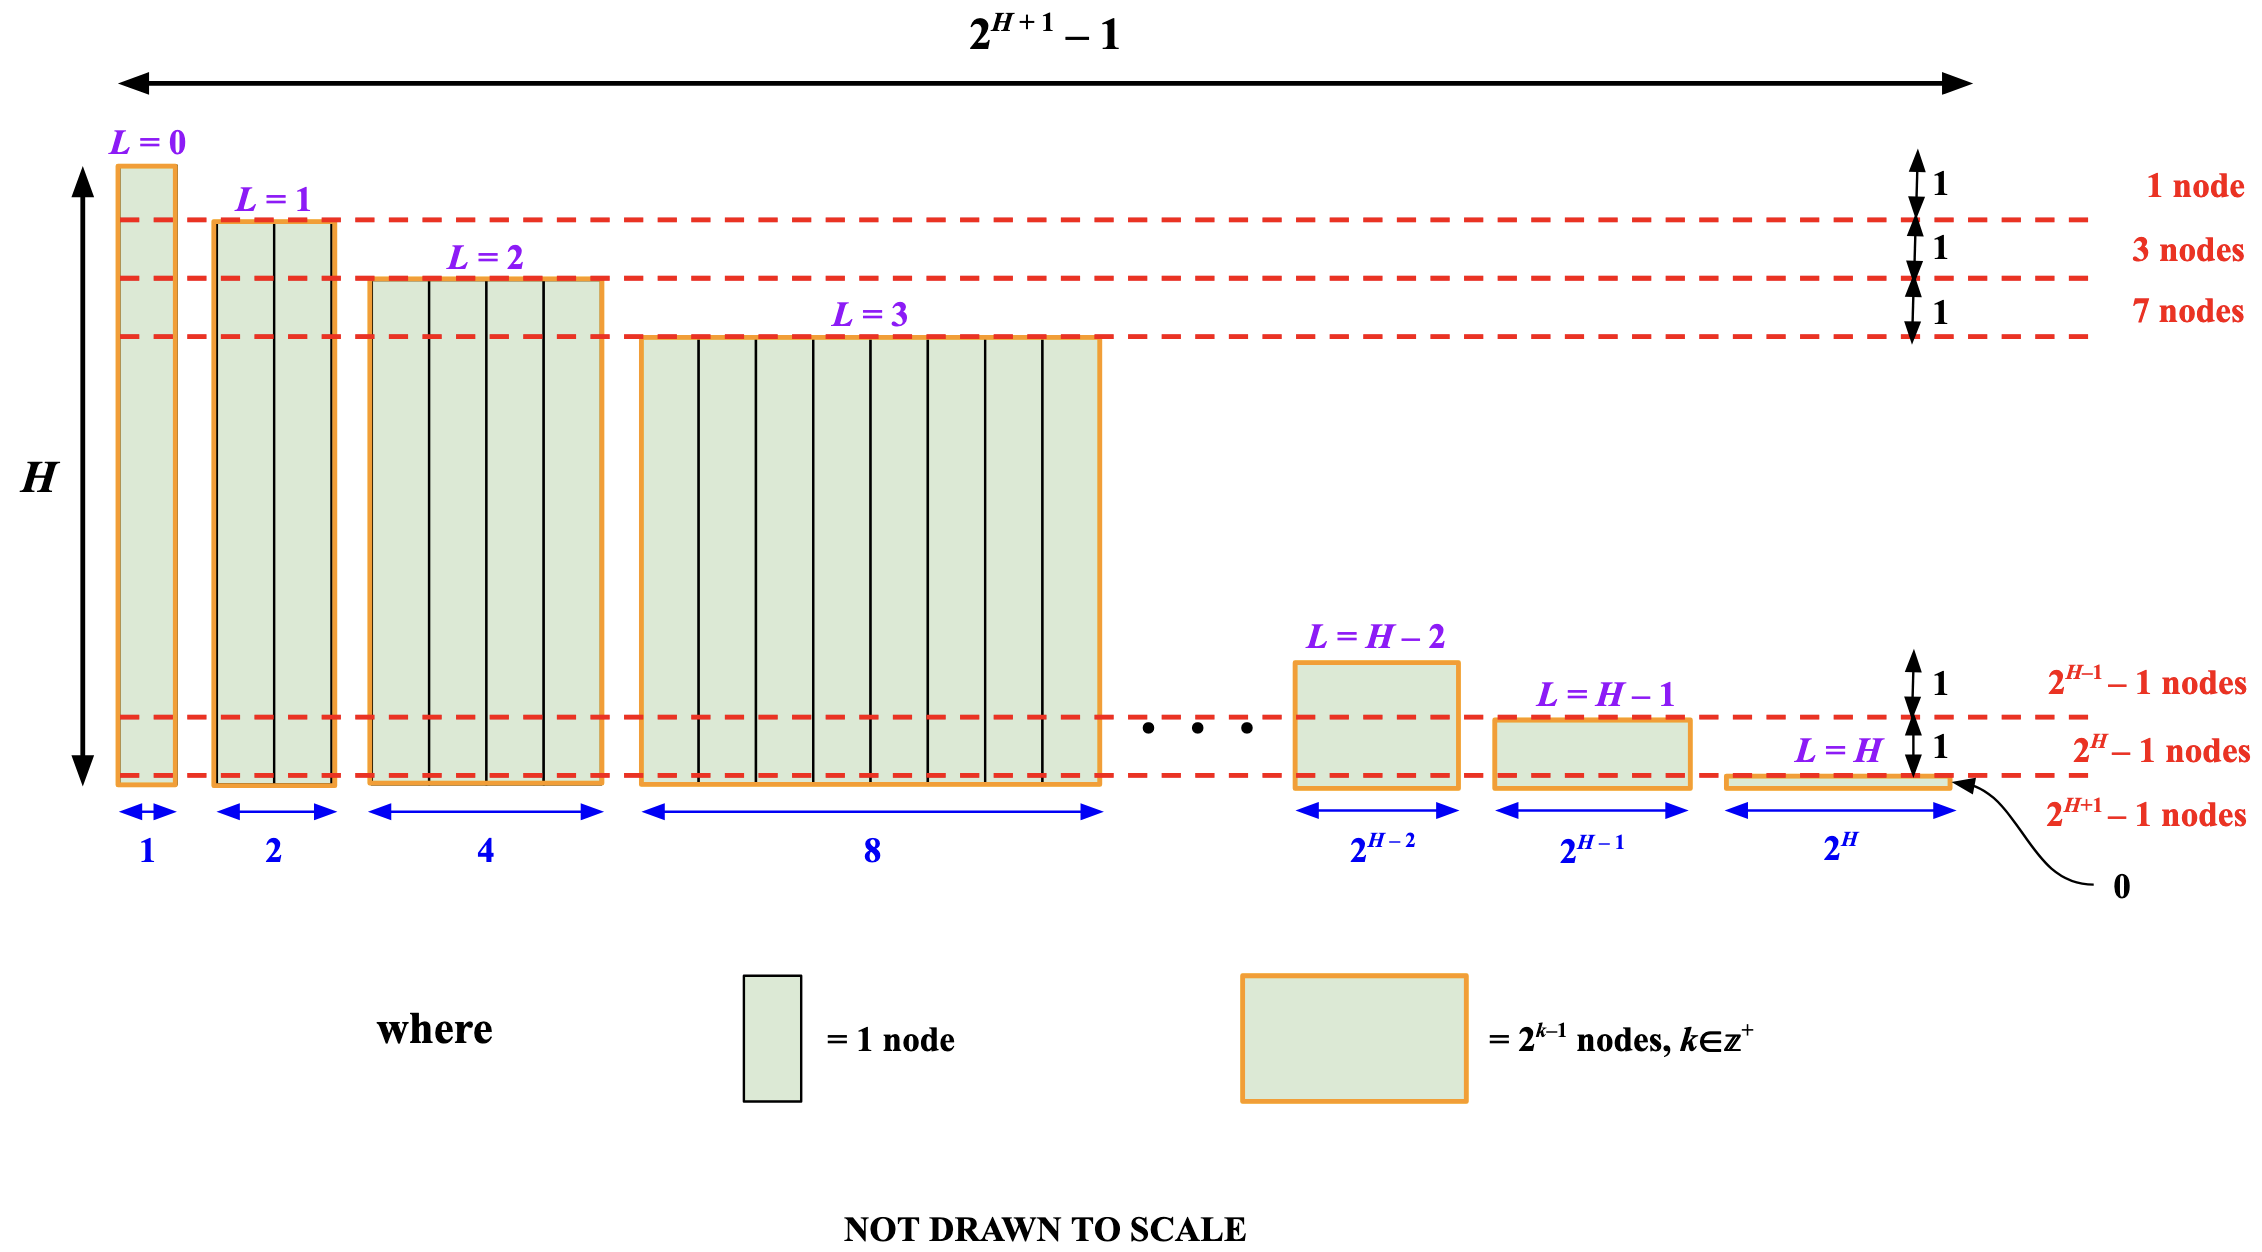
\includegraphics[width=0.9\linewidth]{Google Drawings/floyd-geometric-2-v2.png}
    \label{fig:geo-2-floyd}
\end{figure}

In figure \ref{fig:geo-2-floyd}, I cut the rectangles horizontally into parts of equal height, $1$, since the distance between levels $L$ and $H$ decreases by $1$ as $L$ increases by $1$. Each part is a rectangle of height $1$, or width of $1$ when it is rotated 90 degrees in any direction. Note that the nodes at level $H$ would have a distance to the bottom of the binary heap of $0$.

\begin{figure}[H]
    \centering
    \caption{Representation of cut rectangles from figure \ref{fig:geo-2-floyd}}
    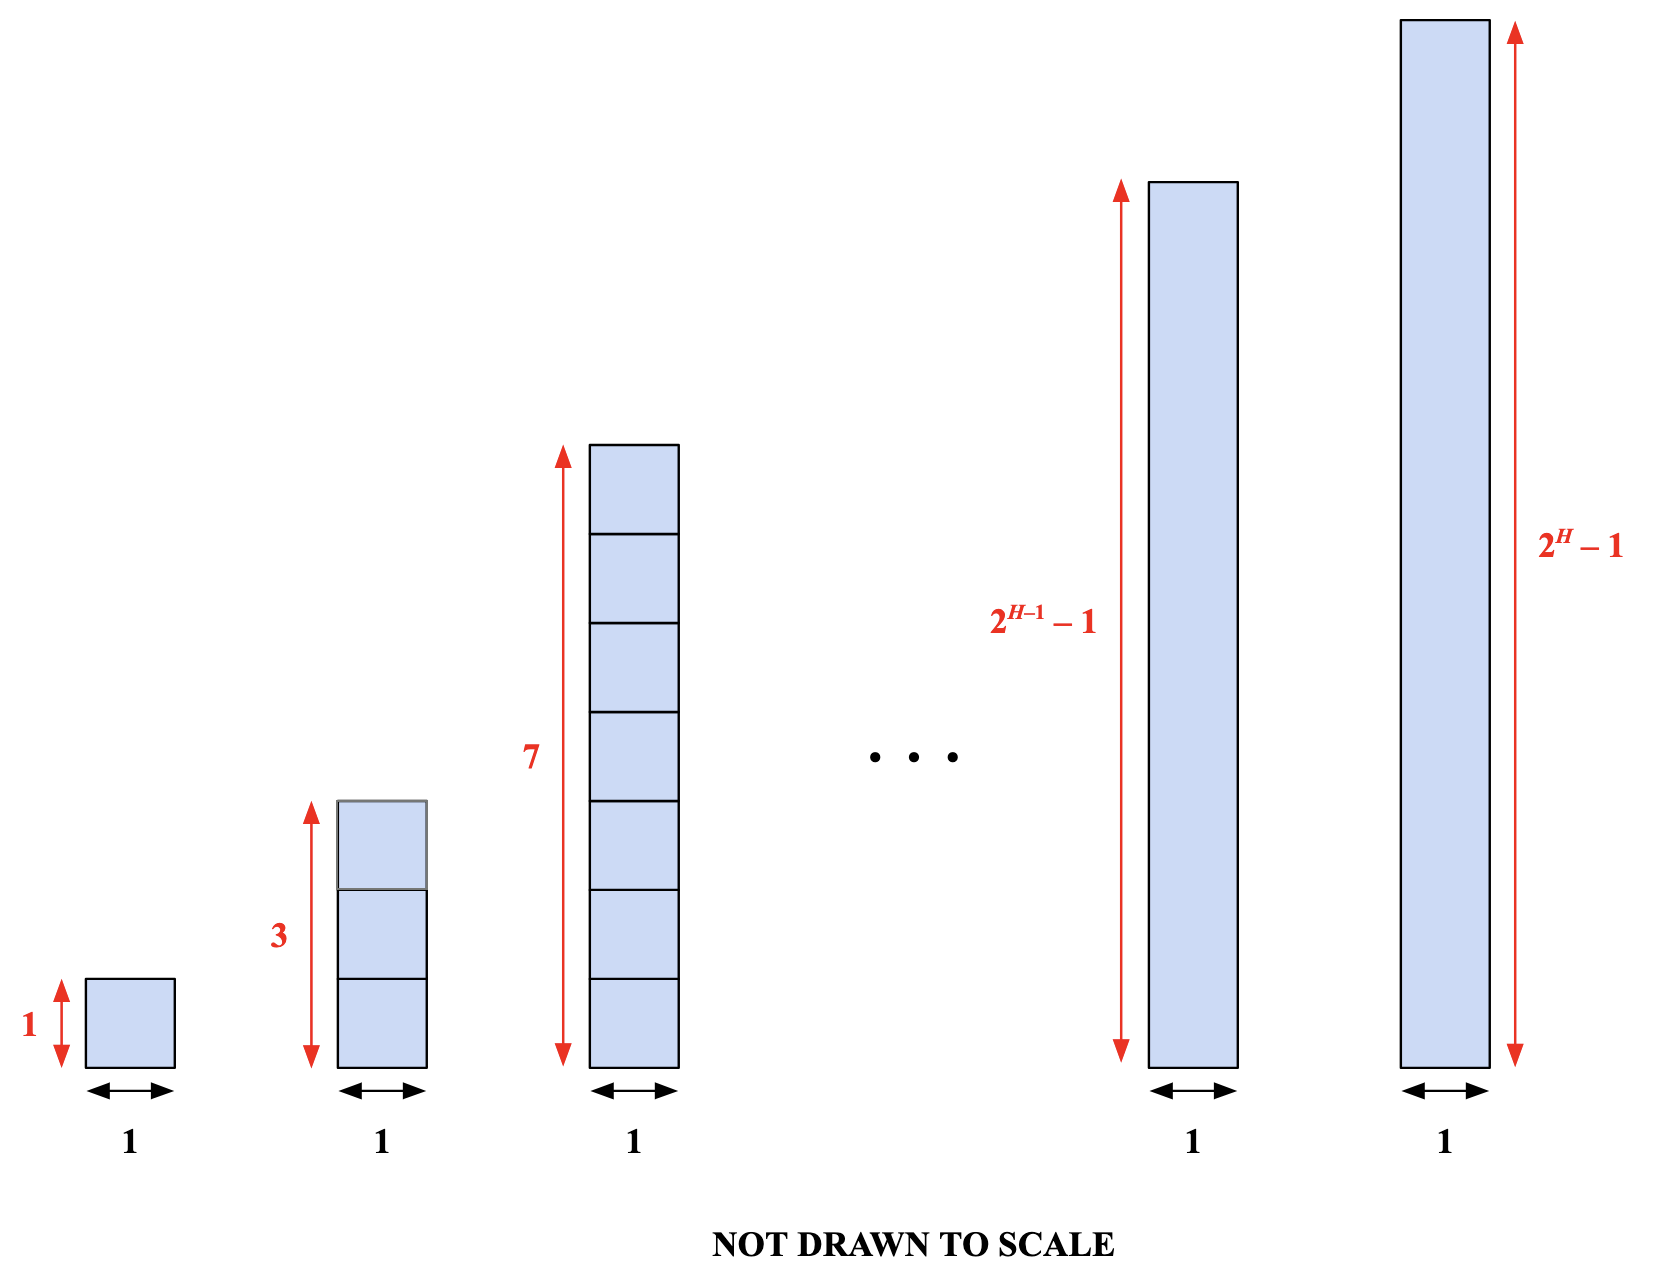
\includegraphics[width=0.75\linewidth]{Google Drawings/floyd-geometric-3-v2.png}
    \label{fig:geo-3-floyd}
\end{figure}

We can now see that the area of figure \ref{fig:geo-3-floyd}, which is the same as that of figure \ref{fig:geo-2-floyd}, can be calculated by applying a summation to $2^H-1$:
\vspace{-2em}

\begin{align*}
    F(H)&=\sum^H_{i=1}(2^i-1)\\
    &=\sum^H_{i=1}(2^i)-H\times 1
\end{align*}

$\sum^H_{i=1}(2^i)$ is a geometric series with a common ratio of $2$. Therefore, I can use the formula for the sum of a geometric series to simplify $F(H)$ and obtain its OOG in the following section.

\subsection{Obtaining the OOG}\label{floyds_OOG}
According to the the \cite{ib}, the formula to find the sum of $n$ terms for a finite geometric series is given as: $S_n=\frac{u_1(r^n-1)}{r-1}$ where $u_1$ is the first term of the series and $r$ is the common ratio of the series. Using this, $F(H)$ and its equivalent function in terms of $N$, $G(N)$, can be simplified:
\vspace{-2em}

\bgroup
\onehalfspacing
\singlespacing
\allowdisplaybreaks
\begin{align*}
    F(H)&=\sum^H_{i=1}(2^i)-H\\
    \phantom{\quad \because S_n=\frac{u_1(r^n-1)}{r-1}}&=\frac{2(2^H-1)}{2-1}-H\quad \because S_n=\frac{u_1(r^n-1)}{r-1}\\
    &=2(2^H-1)-H\\
   \text{Recalling \eqref{eqn:H_ito_N}, }H&=\log_2(N+1)-1\\
    G(N)&\equiv F(H)\\
    &=2(2^{\log_2(N+1)-1}-1)-(\log_2(N+1)-1)\\
    &=2^{\log_2(N+1)-1+1}-2-\log_2(N+1)+1\\
    &=2^{\log_2(N+1)}-1-\log_2(N+1)\\
    &=(N+1)-1-\log_2(N+1)\\
    &=N-\log_2(N+1)\\
    &\therefore \frac{N}{2}<G(N)<N \text{ for large values of } N
\end{align*}
\egroup

Since $G(N)$ is exclusively between $\frac{N}{2}$ and $N$ for large values of $N$, it can be concluded that $G(N)\in O(N)$. Hence, $G(N)$ has been proven to have a linear OOG where $G(N)$ grows in a manner approximately similar to the product of $k$ and $N$ for large values of $N$ with $k$ as some small constant.

\section{Conclusion}\label{conclusion}
When creating a binary heap, Floyd's algorithm is faster than Williams's algorithm since the OOG of the OPS function of Williams's method is $O(N\log{N})$ and the OOG of the OPS function of Floyd's method is $O(N)$. This means that Floyd's method performs less operations for large values of $N$, because the number of operations required to create a binary heap grows slower as $N$ grows, in comparison to Williams's method.\newline

While the speed of Floyd's method has been widely proven, the proofs often require tertiary-level knowledge or calculus \parencites[17]{washu_floyd_proof}[27-28]{skiena_lecture}. In this essay, I have \textbf{found a novel approach} involving the \textbf{transformation of the problem}, seen in figures \ref{fig:geo-1-floyd} to \ref{fig:geo-3-floyd}, using simple sequences and geometry which allows the reason behind Floyd's faster method of creating binary heaps to be \textbf{more easily understood}.

%TC:ignore
\raggedright
\newpage
\printbibliography[
heading=bibnumbered,
title={Bibliography}
]
%TC:endignore
\end{document}
